\documentclass[twoside]{article}

% Packages required by doxygen
\usepackage{fixltx2e}
\usepackage{calc}
\usepackage{doxygen}
\usepackage[export]{adjustbox} % also loads graphicx
\usepackage{graphicx}
\usepackage[utf8]{inputenc}
\usepackage{makeidx}
\usepackage{multicol}
\usepackage{multirow}
\PassOptionsToPackage{warn}{textcomp}
\usepackage{textcomp}
\usepackage[nointegrals]{wasysym}
\usepackage[table]{xcolor}

% Font selection
\usepackage[T1]{fontenc}
\usepackage[scaled=.90]{helvet}
\usepackage{courier}
\usepackage{amssymb}
\usepackage{sectsty}
\renewcommand{\familydefault}{\sfdefault}
\allsectionsfont{%
  \fontseries{bc}\selectfont%
  \color{darkgray}%
}
\renewcommand{\DoxyLabelFont}{%
  \fontseries{bc}\selectfont%
  \color{darkgray}%
}
\newcommand{\+}{\discretionary{\mbox{\scriptsize$\hookleftarrow$}}{}{}}

% Page & text layout
\usepackage{geometry}
\geometry{%
  a4paper,%
  top=2.5cm,%
  bottom=2.5cm,%
  left=2.5cm,%
  right=2.5cm%
}
\tolerance=750
\hfuzz=15pt
\hbadness=750
\setlength{\emergencystretch}{15pt}
\setlength{\parindent}{0cm}
\setlength{\parskip}{0.2cm}
\makeatletter
\renewcommand{\paragraph}{%
  \@startsection{paragraph}{4}{0ex}{-1.0ex}{1.0ex}{%
    \normalfont\normalsize\bfseries\SS@parafont%
  }%
}
\renewcommand{\subparagraph}{%
  \@startsection{subparagraph}{5}{0ex}{-1.0ex}{1.0ex}{%
    \normalfont\normalsize\bfseries\SS@subparafont%
  }%
}
\makeatother

% Headers & footers
\usepackage{fancyhdr}
\pagestyle{fancyplain}
\fancyhead[LE]{\fancyplain{}{\bfseries\thepage}}
\fancyhead[CE]{\fancyplain{}{}}
\fancyhead[RE]{\fancyplain{}{\bfseries\leftmark}}
\fancyhead[LO]{\fancyplain{}{\bfseries\rightmark}}
\fancyhead[CO]{\fancyplain{}{}}
\fancyhead[RO]{\fancyplain{}{\bfseries\thepage}}
\fancyfoot[LE]{\fancyplain{}{}}
\fancyfoot[CE]{\fancyplain{}{}}
\fancyfoot[RE]{\fancyplain{}{\bfseries\scriptsize Generated on Fri May 6 2016 14\+:10\+:35 for Lightstribe W\+S2811/\+W\+S2812 by Doxygen }}
\fancyfoot[LO]{\fancyplain{}{\bfseries\scriptsize Generated on Fri May 6 2016 14\+:10\+:35 for Lightstribe W\+S2811/\+W\+S2812 by Doxygen }}
\fancyfoot[CO]{\fancyplain{}{}}
\fancyfoot[RO]{\fancyplain{}{}}
\renewcommand{\footrulewidth}{0.4pt}
\renewcommand{\sectionmark}[1]{%
  \markright{\thesection\ #1}%
}

% Indices & bibliography
\usepackage{natbib}
\usepackage[titles]{tocloft}
\setcounter{tocdepth}{3}
\setcounter{secnumdepth}{5}
\makeindex

% Hyperlinks (required, but should be loaded last)
\usepackage{ifpdf}
\ifpdf
  \usepackage[pdftex,pagebackref=true]{hyperref}
\else
  \usepackage[ps2pdf,pagebackref=true]{hyperref}
\fi
\hypersetup{%
  colorlinks=true,%
  linkcolor=blue,%
  citecolor=blue,%
  unicode%
}

% Custom commands
\newcommand{\clearemptydoublepage}{%
  \newpage{\pagestyle{empty}\cleardoublepage}%
}


%===== C O N T E N T S =====

\begin{document}

% Titlepage & ToC
\hypersetup{pageanchor=false,
             bookmarks=true,
             bookmarksnumbered=true,
             pdfencoding=unicode
            }
\pagenumbering{roman}
\begin{titlepage}
\vspace*{7cm}
\begin{center}%
{\Large Lightstribe W\+S2811/\+W\+S2812 }\\
\vspace*{1cm}
{\large Generated by Doxygen 1.8.10}\\
\vspace*{0.5cm}
{\small Fri May 6 2016 14:10:35}\\
\end{center}
\end{titlepage}
\tableofcontents
\pagenumbering{arabic}
\hypersetup{pageanchor=true}

%--- Begin generated contents ---
\section{Use W\+S2811/\+W\+S2812 L\+E\+Ds with an A\+V\+R}
\label{index}\hypertarget{index}{} \hypertarget{index_intro_sec}{}\subsection{Introduction}\label{index_intro_sec}
This project is about using an W\+S2811 or W\+S2812 lightstribe with an A\+V\+R controller. It is possible to handle up to 250 L\+E\+Ds at the same time, so I chose an Atmega328p with enough R\+A\+M amount. If you want to handle less L\+E\+Ds you can use most parts of this project with every A\+V\+R. The A\+V\+R is programmed to receive the light data over U\+A\+R\+T so you can control the L\+E\+Ds by using a serial interface. The interface uses a specified simple protocol which is described in \hyperlink{index_protocol_sec}{protocol overview} section. Everything has been developed in a university course to control the lights of a Christmas tree. In the original implementation there were some further components included. This is a simplified version of the implementation so that everyone can use it. As an example for controlling the L\+E\+Ds using a smart phone the \hyperlink{index_esp_sec}{control via E\+S\+P8266} section shows how this could be done by using a webserver on the E\+S\+P8266. You can use everything else that provide a serial interface (maybe connect with a bluetooth serial module). The structure of this documentation is split in a hardware part for the A\+V\+R that describes the basic hardware that should be used. The next part is about how the software is working on the A\+V\+R that handles the L\+E\+Ds and different effects. You may include some more stuff in your own. After that you can see a small protocol overview, where you find which command can be sent to the A\+V\+R to control the L\+E\+Ds. Be aware that at the initialization state all L\+E\+Ds are off. At the last point you can find an example how to use the implementation with an E\+S\+P8266 with a webserver. You will find the source code for the E\+S\+P8266 and the basic hardware setup.\hypertarget{index_hardware_sec}{}\subsection{Hardware}\label{index_hardware_sec}
The basic hardware you need is a A\+V\+R controller an some W\+S2811 or W\+S2812 L\+E\+Ds you want to control. The A\+V\+R controller should have an hardware U\+A\+R\+T, otherwise you need to write some code for a software serial. In the project we chose an Atmega328p that has enough R\+A\+M to control 250 L\+E\+Ds. The internal software structure buffers the color data for the L\+E\+Ds to achieve an accurate timing, see section \hyperlink{index_software_sec}{software implementation}. The A\+V\+R can be used with the internal clock at 8 M\+Hz, remember to clear the clock divider fuse. Otherwise an external 8 M\+Hz or 16 M\+Hz clock source can be used, the definition \hyperlink{globals_8h_a43bafb28b29491ec7f871319b5a3b2f8}{F\+\_\+\+C\+P\+U} must be set to the frequency you chose (remember to set the fuses for an external clock source). As an example the figure \hyperlink{index_one}{one} shows using an external 16 M\+Hz crystal. \label{index_one}%
\hypertarget{index_one}{}%

\begin{DoxyImage}
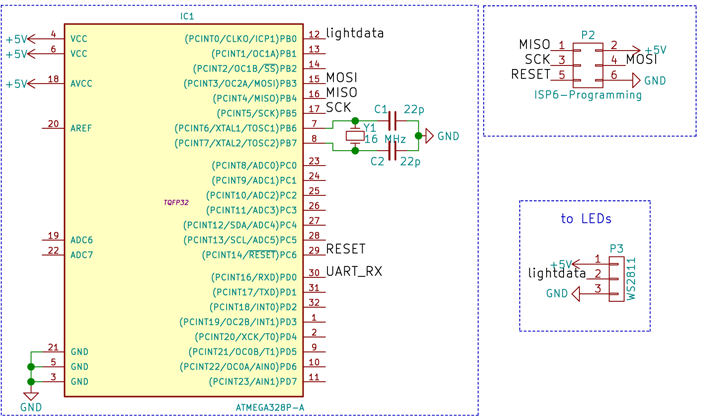
\includegraphics[width=\textwidth,height=\textheight/2,keepaspectratio=true]{Ws2811_Atmega328_schematic.png}
\caption{schematic of the A\+V\+R to controll W\+S2812/\+W\+S2811}
\end{DoxyImage}
 As you can see in the picture the A\+V\+R is programmed by using the I\+S\+P interface. The W\+S2812/\+W\+S2811 get the same voltage as the A\+V\+R, the light data is available at Pin\+B0, you may change this if you like. Referring to the L\+E\+Ds be aware of the current amount they may draw if every L\+E\+D has its full brightness. One W\+S2812 can draw up to 60 m\+A, so one meter with 30 L\+E\+Ds already need 1,8 A. If you want to control more L\+E\+Ds you may have a problem with the voltage drop along the stribe. For example if you control 180 L\+E\+Ds at six meters you not only need 10,8 A, furthermore you will probably have a voltage drop up to 2 V. To reduce the voltage drop you must increase the wire size with parallel wires to you stribe. You can see the voltage drop if you set all L\+E\+Ds to white. If you have only a small voltage drop every L\+E\+D will have the same color. If the voltage drop is too much you can see that the last L\+E\+Ds will have less blue color, so they will light in a warm white color even up to red. If you want to try out the L\+E\+Ds with the A\+V\+R you can build up everything on a breadboard. Pinheaders can be soldered easy at the light stribes as you can see in the figure \hyperlink{index_two}{two}. \label{index_two}%
\hypertarget{index_two}{}%

\begin{DoxyImage}
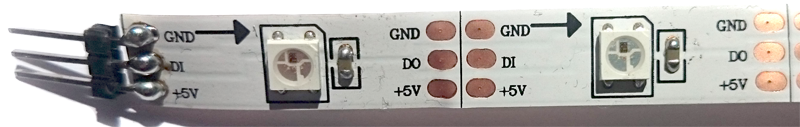
\includegraphics[width=\textwidth,height=\textheight/2,keepaspectratio=true]{WS2812.png}
\caption{W\+S2812 stribe with pin header}
\end{DoxyImage}
The connect G\+N\+D to the common ground with the A\+V\+R, 5 V should be connected to a power supply that can handle the current you need. D\+I is the data in line, this should be connected to Pin\+B0 at the A\+V\+R. The stribe is like a big shifting register, all the data you sent is shifted bit by bit through the stribe. So D\+O is the data out pin, you see some data at this pin if all L\+E\+Ds before had already received their color data. The one wire protocol of the L\+E\+Ds is described in the \hyperlink{index_software_sec}{software implementation} section.\hypertarget{index_software_sec}{}\subsection{software implementation}\label{index_software_sec}
\hypertarget{index_install_sec}{}\subsection{Installation}\label{index_install_sec}
\hypertarget{index_step1}{}\subsubsection{Step 1\+: Opening the box}\label{index_step1}
etc...\hypertarget{index_protocol_sec}{}\subsection{protocol overview}\label{index_protocol_sec}
\hypertarget{index_esp_sec}{}\subsection{control via E\+S\+P8266}\label{index_esp_sec}
author\+: Florian Wank, 2016 
\section{Data Structure Index}
\subsection{Data Structures}
Here are the data structures with brief descriptions\+:\begin{DoxyCompactList}
\item\contentsline{section}{\hyperlink{structcolor24bit}{color24bit} \\*24 Bit color structure R\+G\+B 8-\/8-\/8 }{\pageref{structcolor24bit}}{}
\end{DoxyCompactList}

\section{File Index}
\subsection{File List}
Here is a list of all documented files with brief descriptions\+:\begin{DoxyCompactList}
\item\contentsline{section}{\hyperlink{globals_8h}{globals.\+h} \\*File that contains basic and global definitions, changes should be done carefully }{\pageref{globals_8h}}{}
\item\contentsline{section}{\hyperlink{_led_effects_8c}{Led\+Effects.\+c} \\*Effect functions for controlling W\+S2811/\+W\+S2812 L\+E\+Ds }{\pageref{_led_effects_8c}}{}
\item\contentsline{section}{\hyperlink{_led_effects_8h}{Led\+Effects.\+h} \\*File that contains different effect definitions for the lightstribe }{\pageref{_led_effects_8h}}{}
\item\contentsline{section}{\hyperlink{_lightstribe_8c}{Lightstribe.\+c} \\*Basic functions for controlling W\+S2811/\+W\+S2812 L\+E\+Ds }{\pageref{_lightstribe_8c}}{}
\item\contentsline{section}{\hyperlink{_lightstribe_8h}{Lightstribe.\+h} \\*Basic functions for controlling W\+S2811/\+W\+S2812 L\+E\+Ds }{\pageref{_lightstribe_8h}}{}
\item\contentsline{section}{\hyperlink{ws2811lichterkette_8c}{ws2811lichterkette.\+c} \\*Main file for interfacing W\+S2811/\+W\+S2812 L\+E\+Ds }{\pageref{ws2811lichterkette_8c}}{}
\end{DoxyCompactList}

\section{Data Structure Documentation}
\hypertarget{structcolor24bit}{}\subsection{color24bit Struct Reference}
\label{structcolor24bit}\index{color24bit@{color24bit}}


24 Bit color structure R\+G\+B 8-\/8-\/8  




{\ttfamily \#include $<$Lightstribe.\+h$>$}

\subsubsection*{Data Fields}
\begin{DoxyCompactItemize}
\item 
uint8\+\_\+t \hyperlink{structcolor24bit_ad47d918910aaa51c73160ac85999d09c}{red}
\item 
uint8\+\_\+t \hyperlink{structcolor24bit_a90d21fa503b626c00cdc8d94863d5877}{green}
\item 
uint8\+\_\+t \hyperlink{structcolor24bit_a287b397e90d7b995c81ff54e741f96b2}{blue}
\end{DoxyCompactItemize}


\subsubsection{Detailed Description}
24 Bit color structure R\+G\+B 8-\/8-\/8 

Definition at line \hyperlink{_lightstribe_8h_source_l00016}{16} of file \hyperlink{_lightstribe_8h_source}{Lightstribe.\+h}.



\subsubsection{Field Documentation}
\hypertarget{structcolor24bit_a287b397e90d7b995c81ff54e741f96b2}{}\index{color24bit@{color24bit}!blue@{blue}}
\index{blue@{blue}!color24bit@{color24bit}}
\paragraph[{blue}]{\setlength{\rightskip}{0pt plus 5cm}uint8\+\_\+t blue}\label{structcolor24bit_a287b397e90d7b995c81ff54e741f96b2}
8 Bit blue 

Definition at line \hyperlink{_lightstribe_8h_source_l00019}{19} of file \hyperlink{_lightstribe_8h_source}{Lightstribe.\+h}.



Referenced by \hyperlink{_lightstribe_8c_source_l00033}{changeled()}, \hyperlink{_led_effects_8c_source_l00045}{colorconv8to24()}, \hyperlink{_led_effects_8c_source_l00366}{faden()}, \hyperlink{_led_effects_8c_source_l00442}{initrainbow()}, \hyperlink{_led_effects_8c_source_l00118}{resetstribe()}, \hyperlink{_led_effects_8c_source_l00096}{setfullcolor()}, and \hyperlink{_lightstribe_8c_source_l00051}{setled()}.

\hypertarget{structcolor24bit_a90d21fa503b626c00cdc8d94863d5877}{}\index{color24bit@{color24bit}!green@{green}}
\index{green@{green}!color24bit@{color24bit}}
\paragraph[{green}]{\setlength{\rightskip}{0pt plus 5cm}uint8\+\_\+t green}\label{structcolor24bit_a90d21fa503b626c00cdc8d94863d5877}
8 Bit green 

Definition at line \hyperlink{_lightstribe_8h_source_l00018}{18} of file \hyperlink{_lightstribe_8h_source}{Lightstribe.\+h}.



Referenced by \hyperlink{_lightstribe_8c_source_l00033}{changeled()}, \hyperlink{_led_effects_8c_source_l00045}{colorconv8to24()}, \hyperlink{_led_effects_8c_source_l00366}{faden()}, \hyperlink{_led_effects_8c_source_l00442}{initrainbow()}, \hyperlink{_led_effects_8c_source_l00118}{resetstribe()}, \hyperlink{_led_effects_8c_source_l00096}{setfullcolor()}, and \hyperlink{_lightstribe_8c_source_l00051}{setled()}.

\hypertarget{structcolor24bit_ad47d918910aaa51c73160ac85999d09c}{}\index{color24bit@{color24bit}!red@{red}}
\index{red@{red}!color24bit@{color24bit}}
\paragraph[{red}]{\setlength{\rightskip}{0pt plus 5cm}uint8\+\_\+t red}\label{structcolor24bit_ad47d918910aaa51c73160ac85999d09c}
8 Bit red 

Definition at line \hyperlink{_lightstribe_8h_source_l00017}{17} of file \hyperlink{_lightstribe_8h_source}{Lightstribe.\+h}.



Referenced by \hyperlink{_lightstribe_8c_source_l00033}{changeled()}, \hyperlink{_led_effects_8c_source_l00045}{colorconv8to24()}, \hyperlink{_led_effects_8c_source_l00366}{faden()}, \hyperlink{_led_effects_8c_source_l00442}{initrainbow()}, \hyperlink{_led_effects_8c_source_l00118}{resetstribe()}, \hyperlink{_led_effects_8c_source_l00096}{setfullcolor()}, and \hyperlink{_lightstribe_8c_source_l00051}{setled()}.



The documentation for this struct was generated from the following file\+:\begin{DoxyCompactItemize}
\item 
\hyperlink{_lightstribe_8h}{Lightstribe.\+h}\end{DoxyCompactItemize}

\section{File Documentation}
\hypertarget{globals_8h}{}\subsection{globals.\+h File Reference}
\label{globals_8h}\index{globals.\+h@{globals.\+h}}


file that contains basic and global definitions, no changes should be done here  


{\ttfamily \#include $<$stdint.\+h$>$}\\*
\subsubsection*{Macros}
\begin{DoxyCompactItemize}
\item 
\hypertarget{globals_8h_a9b1581d45c3729eba4966b893457d148}{}\#define {\bfseries \+\_\+\+S\+T\+R\+\_\+\+E\+X\+P\+A\+N\+D}(tok)~\#tok\label{globals_8h_a9b1581d45c3729eba4966b893457d148}

\item 
\hypertarget{globals_8h_a3976b857dc3fc0e3627b3a6b28062299}{}\#define {\bfseries \+\_\+\+S\+T\+R}(tok)~\+\_\+\+S\+T\+R\+\_\+\+E\+X\+P\+A\+N\+D(tok)\label{globals_8h_a3976b857dc3fc0e3627b3a6b28062299}

\item 
\hypertarget{globals_8h_a1190af2e5eb5d640bf7e59588deddddf}{}\#define {\bfseries \+\_\+\+C\+P\+U\+\_\+\+I\+N\+F\+O}(x)~C\+P\+U\+\_\+\+F\+R\+E\+Q\+U\+E\+N\+C\+Y\#\#x\label{globals_8h_a1190af2e5eb5d640bf7e59588deddddf}

\item 
\hypertarget{globals_8h_a77366c1bd428629dc898e188bfd182a3}{}\#define \hyperlink{globals_8h_a77366c1bd428629dc898e188bfd182a3}{E\+X\+T\+E\+R\+N}~extern\label{globals_8h_a77366c1bd428629dc898e188bfd182a3}

\begin{DoxyCompactList}\small\item\em macro for global variable management \end{DoxyCompactList}\item 
\hypertarget{globals_8h_af07a5ce170c7be13d096843960e7b9da}{}\#define \hyperlink{globals_8h_af07a5ce170c7be13d096843960e7b9da}{B\+A\+S\+E\+L\+E\+D\+T\+Y\+P\+E}~11\label{globals_8h_af07a5ce170c7be13d096843960e7b9da}

\begin{DoxyCompactList}\small\item\em default L\+E\+D type of the stribe (11 for W\+S2811, do not change here! change ledtype in main function!) \end{DoxyCompactList}\item 
\hypertarget{globals_8h_a6e2b9e79df9491377ae405ef85aa0ca5}{}\#define \hyperlink{globals_8h_a6e2b9e79df9491377ae405ef85aa0ca5}{M\+A\+X\+N\+U\+M\+C\+O\+L\+O\+R\+S}~50\label{globals_8h_a6e2b9e79df9491377ae405ef85aa0ca5}

\begin{DoxyCompactList}\small\item\em definition for maximum number of different colors that can be handled at the same time (the maximum value should be 50, a higher value may result in an memory overflow refering to 2k\+Byte (atmega328p)) \end{DoxyCompactList}\item 
\hypertarget{globals_8h_a0d57378e32bf8278011460740bc29f7f}{}\#define \hyperlink{globals_8h_a0d57378e32bf8278011460740bc29f7f}{U\+A\+R\+T\+\_\+\+B\+U\+F\+F\+E\+R\+\_\+\+S\+I\+Z\+E}~80\label{globals_8h_a0d57378e32bf8278011460740bc29f7f}

\begin{DoxyCompactList}\small\item\em definition for U\+A\+R\+T Buffer, must be at least M\+A\+X\+N\+U\+M\+C\+O\+L\+O\+R\+S+5 \end{DoxyCompactList}\item 
\hypertarget{globals_8h_a43bafb28b29491ec7f871319b5a3b2f8}{}\#define \hyperlink{globals_8h_a43bafb28b29491ec7f871319b5a3b2f8}{F\+\_\+\+C\+P\+U}~8000000\label{globals_8h_a43bafb28b29491ec7f871319b5a3b2f8}

\begin{DoxyCompactList}\small\item\em C\+P\+U Frequency definition for avr delay function. \end{DoxyCompactList}\end{DoxyCompactItemize}
\subsubsection*{Variables}
\begin{DoxyCompactItemize}
\item 
\hypertarget{globals_8h_ad5db4045aed262ed4aae2af9d81fab98}{}\hyperlink{globals_8h_a77366c1bd428629dc898e188bfd182a3}{E\+X\+T\+E\+R\+N} uint8\+\_\+t \hyperlink{globals_8h_ad5db4045aed262ed4aae2af9d81fab98}{Num\+Of\+Leds}\label{globals_8h_ad5db4045aed262ed4aae2af9d81fab98}

\begin{DoxyCompactList}\small\item\em global variable for number of leds to control \end{DoxyCompactList}\item 
\hypertarget{globals_8h_ac2445d316b2972d381edeac44bb6a226}{}\hyperlink{globals_8h_a77366c1bd428629dc898e188bfd182a3}{E\+X\+T\+E\+R\+N} uint16\+\_\+t \hyperlink{globals_8h_ac2445d316b2972d381edeac44bb6a226}{effectime}\label{globals_8h_ac2445d316b2972d381edeac44bb6a226}

\begin{DoxyCompactList}\small\item\em global effectime for effect delays, a higher value means a higher delay \end{DoxyCompactList}\item 
\hypertarget{globals_8h_a722e1eb38b661d1338ada3cc7a4049a0}{}\hyperlink{globals_8h_a77366c1bd428629dc898e188bfd182a3}{E\+X\+T\+E\+R\+N} uint8\+\_\+t \hyperlink{globals_8h_a722e1eb38b661d1338ada3cc7a4049a0}{ledtype}\label{globals_8h_a722e1eb38b661d1338ada3cc7a4049a0}

\begin{DoxyCompactList}\small\item\em global ledtype, 11 = W\+S2811 (R\+G\+B Color), 12 = W\+S2812 (G\+R\+B Color) \end{DoxyCompactList}\item 
\hypertarget{globals_8h_a159854edb9d0c7283013495d85bdf997}{}\hyperlink{globals_8h_a77366c1bd428629dc898e188bfd182a3}{E\+X\+T\+E\+R\+N} uint8\+\_\+t \hyperlink{globals_8h_a159854edb9d0c7283013495d85bdf997}{Comp\+Color\+Array} \mbox{[}\hyperlink{globals_8h_a6e2b9e79df9491377ae405ef85aa0ca5}{M\+A\+X\+N\+U\+M\+C\+O\+L\+O\+R\+S}\mbox{]}\label{globals_8h_a159854edb9d0c7283013495d85bdf997}

\begin{DoxyCompactList}\small\item\em color array containing the received packed 8-\/\+Bit colors \end{DoxyCompactList}\item 
\hypertarget{globals_8h_a5d735865707e6694a8173d629e0b4d5c}{}\hyperlink{globals_8h_a77366c1bd428629dc898e188bfd182a3}{E\+X\+T\+E\+R\+N} uint8\+\_\+t \hyperlink{globals_8h_a5d735865707e6694a8173d629e0b4d5c}{Rec\+Buffer} \mbox{[}\hyperlink{globals_8h_a0d57378e32bf8278011460740bc29f7f}{U\+A\+R\+T\+\_\+\+B\+U\+F\+F\+E\+R\+\_\+\+S\+I\+Z\+E}\mbox{]}\label{globals_8h_a5d735865707e6694a8173d629e0b4d5c}

\begin{DoxyCompactList}\small\item\em receive buffer for U\+A\+R\+T communication \end{DoxyCompactList}\item 
\hypertarget{globals_8h_aa6fcb4d4fca4554ac73bef10668c23cd}{}\hyperlink{globals_8h_a77366c1bd428629dc898e188bfd182a3}{E\+X\+T\+E\+R\+N} uint8\+\_\+t \hyperlink{globals_8h_aa6fcb4d4fca4554ac73bef10668c23cd}{Buffer\+Counter}\label{globals_8h_aa6fcb4d4fca4554ac73bef10668c23cd}

\begin{DoxyCompactList}\small\item\em counter for accessing the Comp\+Color\+Array indices for data income \end{DoxyCompactList}\item 
\hypertarget{globals_8h_aaa611e00c18e950be43a4cd5ce0ceeb1}{}\hyperlink{globals_8h_a77366c1bd428629dc898e188bfd182a3}{E\+X\+T\+E\+R\+N} uint8\+\_\+t \hyperlink{globals_8h_aaa611e00c18e950be43a4cd5ce0ceeb1}{Data\+Len}\label{globals_8h_aaa611e00c18e950be43a4cd5ce0ceeb1}

\begin{DoxyCompactList}\small\item\em variable to store the current packet length of the U\+A\+R\+T packet \end{DoxyCompactList}\item 
\hypertarget{globals_8h_a053b8e1f039c19251b90d60317db8aed}{}\hyperlink{globals_8h_a77366c1bd428629dc898e188bfd182a3}{E\+X\+T\+E\+R\+N} uint8\+\_\+t \hyperlink{globals_8h_a053b8e1f039c19251b90d60317db8aed}{effect}\label{globals_8h_a053b8e1f039c19251b90d60317db8aed}

\begin{DoxyCompactList}\small\item\em global effect variable to switch between the effects \end{DoxyCompactList}\item 
\hypertarget{globals_8h_a1b09d1a5bcf4c8ab435bb3c9e36def59}{}\hyperlink{globals_8h_a77366c1bd428629dc898e188bfd182a3}{E\+X\+T\+E\+R\+N} uint8\+\_\+t \hyperlink{globals_8h_a1b09d1a5bcf4c8ab435bb3c9e36def59}{Packet\+Complete}\label{globals_8h_a1b09d1a5bcf4c8ab435bb3c9e36def59}

\begin{DoxyCompactList}\small\item\em flag to store if a U\+A\+R\+T packet is complete; a packet is complete if the Buffer\+Counter equals Data\+Len \end{DoxyCompactList}\item 
\hypertarget{globals_8h_aaa3bddd2273257ac5ec259197b62e984}{}\hyperlink{globals_8h_a77366c1bd428629dc898e188bfd182a3}{E\+X\+T\+E\+R\+N} uint8\+\_\+t \hyperlink{globals_8h_aaa3bddd2273257ac5ec259197b62e984}{Paket\+Start}\label{globals_8h_aaa3bddd2273257ac5ec259197b62e984}

\begin{DoxyCompactList}\small\item\em flag to store if the \hyperlink{ws2811lichterkette_8c_a8aac8c5098aaf915463fb31715efa09f}{P\+R\+E\+A\+M\+B\+L\+E} has been received \end{DoxyCompactList}\item 
\hypertarget{globals_8h_a922ad5baed647eca43ad1a979e162ebd}{}\hyperlink{globals_8h_a77366c1bd428629dc898e188bfd182a3}{E\+X\+T\+E\+R\+N} uint8\+\_\+t \hyperlink{globals_8h_a922ad5baed647eca43ad1a979e162ebd}{Is\+Reading}\label{globals_8h_a922ad5baed647eca43ad1a979e162ebd}

\begin{DoxyCompactList}\small\item\em flag to show if the Rec\+Buffer is in copy process so that the array cannot be filled with new data from U\+A\+R\+T \end{DoxyCompactList}\item 
\hypertarget{globals_8h_ab5490074aaca289e986e9a00e0c25663}{}\hyperlink{globals_8h_a77366c1bd428629dc898e188bfd182a3}{E\+X\+T\+E\+R\+N} volatile char \hyperlink{globals_8h_ab5490074aaca289e986e9a00e0c25663}{Received\+Char}\label{globals_8h_ab5490074aaca289e986e9a00e0c25663}

\begin{DoxyCompactList}\small\item\em current data received from U\+A\+R\+T \end{DoxyCompactList}\end{DoxyCompactItemize}


\subsubsection{Detailed Description}
file that contains basic and global definitions, no changes should be done here 

\begin{DoxyVersion}{Version}
V1.\+00 
\end{DoxyVersion}
\begin{DoxyDate}{Date}
05.\+01.\+2016 
\end{DoxyDate}
\begin{DoxyAuthor}{Authors}
Wank Florian 
\end{DoxyAuthor}


Definition in file \hyperlink{globals_8h_source}{globals.\+h}.


\hypertarget{globals_8h_source}{}\subsection{globals.\+h}

\begin{DoxyCode}
00001 \textcolor{comment}{/**************************************************************************/}
00009 \textcolor{preprocessor}{#include <stdint.h>}
00010 
00011 \textcolor{preprocessor}{#ifndef GLOBALS\_H\_}
00012 \textcolor{preprocessor}{#define GLOBALS\_H\_}
00013 
00014 \textcolor{comment}{//macros to display infos for CPU Frequency or other defines}
00015 \textcolor{preprocessor}{#define \_STR\_EXPAND(tok) #tok}
00016 \textcolor{preprocessor}{#define \_STR(tok) \_STR\_EXPAND(tok)}
00017 \textcolor{preprocessor}{#define \_CPU\_INFO(x) CPU\_FREQUENCY##x}
00018 
00020 \textcolor{preprocessor}{#ifndef EXTERN}
\hypertarget{globals_8h_source_l00021}{}\hyperlink{globals_8h_a77366c1bd428629dc898e188bfd182a3}{00021} \textcolor{preprocessor}{#define EXTERN extern}
00022 \textcolor{preprocessor}{#endif}
00023 
\hypertarget{globals_8h_source_l00025}{}\hyperlink{globals_8h_ad5db4045aed262ed4aae2af9d81fab98}{00025} \hyperlink{globals_8h_a77366c1bd428629dc898e188bfd182a3}{EXTERN} uint8\_t \hyperlink{globals_8h_ad5db4045aed262ed4aae2af9d81fab98}{NumOfLeds};
\hypertarget{globals_8h_source_l00027}{}\hyperlink{globals_8h_ac2445d316b2972d381edeac44bb6a226}{00027} \hyperlink{globals_8h_a77366c1bd428629dc898e188bfd182a3}{EXTERN} uint16\_t \hyperlink{globals_8h_ac2445d316b2972d381edeac44bb6a226}{effectime};
\hypertarget{globals_8h_source_l00029}{}\hyperlink{globals_8h_a722e1eb38b661d1338ada3cc7a4049a0}{00029} \hyperlink{globals_8h_a77366c1bd428629dc898e188bfd182a3}{EXTERN} uint8\_t \hyperlink{globals_8h_a722e1eb38b661d1338ada3cc7a4049a0}{ledtype};
\hypertarget{globals_8h_source_l00031}{}\hyperlink{globals_8h_af07a5ce170c7be13d096843960e7b9da}{00031} \textcolor{preprocessor}{#define BASELEDTYPE 11}
00032 
\hypertarget{globals_8h_source_l00035}{}\hyperlink{globals_8h_a6e2b9e79df9491377ae405ef85aa0ca5}{00035} \textcolor{preprocessor}{#define MAXNUMCOLORS 50}
00036 
\hypertarget{globals_8h_source_l00037}{}\hyperlink{globals_8h_a0d57378e32bf8278011460740bc29f7f}{00037} \textcolor{preprocessor}{#define UART\_BUFFER\_SIZE 80}
00038 
\hypertarget{globals_8h_source_l00040}{}\hyperlink{globals_8h_a159854edb9d0c7283013495d85bdf997}{00040} \hyperlink{globals_8h_a77366c1bd428629dc898e188bfd182a3}{EXTERN} uint8\_t \hyperlink{globals_8h_a159854edb9d0c7283013495d85bdf997}{CompColorArray}[\hyperlink{globals_8h_a6e2b9e79df9491377ae405ef85aa0ca5}{MAXNUMCOLORS}];
\hypertarget{globals_8h_source_l00042}{}\hyperlink{globals_8h_a5d735865707e6694a8173d629e0b4d5c}{00042} \hyperlink{globals_8h_a77366c1bd428629dc898e188bfd182a3}{EXTERN} uint8\_t \hyperlink{globals_8h_a5d735865707e6694a8173d629e0b4d5c}{RecBuffer}[\hyperlink{globals_8h_a0d57378e32bf8278011460740bc29f7f}{UART\_BUFFER\_SIZE}];
\hypertarget{globals_8h_source_l00044}{}\hyperlink{globals_8h_aa6fcb4d4fca4554ac73bef10668c23cd}{00044} \hyperlink{globals_8h_a77366c1bd428629dc898e188bfd182a3}{EXTERN} uint8\_t \hyperlink{globals_8h_aa6fcb4d4fca4554ac73bef10668c23cd}{BufferCounter};
\hypertarget{globals_8h_source_l00046}{}\hyperlink{globals_8h_aaa611e00c18e950be43a4cd5ce0ceeb1}{00046} \hyperlink{globals_8h_a77366c1bd428629dc898e188bfd182a3}{EXTERN} uint8\_t \hyperlink{globals_8h_aaa611e00c18e950be43a4cd5ce0ceeb1}{DataLen};
\hypertarget{globals_8h_source_l00048}{}\hyperlink{globals_8h_a053b8e1f039c19251b90d60317db8aed}{00048} \hyperlink{globals_8h_a77366c1bd428629dc898e188bfd182a3}{EXTERN} uint8\_t \hyperlink{globals_8h_a053b8e1f039c19251b90d60317db8aed}{effect};
00049 
00050 \textcolor{comment}{//EXTERN uint8\_t speed;}
00051 
\hypertarget{globals_8h_source_l00053}{}\hyperlink{globals_8h_a1b09d1a5bcf4c8ab435bb3c9e36def59}{00053} \hyperlink{globals_8h_a77366c1bd428629dc898e188bfd182a3}{EXTERN} uint8\_t \hyperlink{globals_8h_a1b09d1a5bcf4c8ab435bb3c9e36def59}{PacketComplete};
\hypertarget{globals_8h_source_l00055}{}\hyperlink{globals_8h_aaa3bddd2273257ac5ec259197b62e984}{00055} \hyperlink{globals_8h_a77366c1bd428629dc898e188bfd182a3}{EXTERN} uint8\_t \hyperlink{globals_8h_aaa3bddd2273257ac5ec259197b62e984}{PaketStart};
\hypertarget{globals_8h_source_l00057}{}\hyperlink{globals_8h_a922ad5baed647eca43ad1a979e162ebd}{00057} \hyperlink{globals_8h_a77366c1bd428629dc898e188bfd182a3}{EXTERN} uint8\_t \hyperlink{globals_8h_a922ad5baed647eca43ad1a979e162ebd}{IsReading};
\hypertarget{globals_8h_source_l00059}{}\hyperlink{globals_8h_ab5490074aaca289e986e9a00e0c25663}{00059} \hyperlink{globals_8h_a77366c1bd428629dc898e188bfd182a3}{EXTERN} \textcolor{keyword}{volatile} \textcolor{keywordtype}{char} \hyperlink{globals_8h_ab5490074aaca289e986e9a00e0c25663}{ReceivedChar};
00060 
00062 \textcolor{preprocessor}{#ifndef F\_CPU}
\hypertarget{globals_8h_source_l00063}{}\hyperlink{globals_8h_a43bafb28b29491ec7f871319b5a3b2f8}{00063} \textcolor{preprocessor}{#define F\_CPU 8000000}
00064 \textcolor{preprocessor}{#endif}
00065 \textcolor{preprocessor}{#endif }\textcolor{comment}{/* GLOBALS\_H\_ */}\textcolor{preprocessor}{}
\end{DoxyCode}

\hypertarget{_led_effects_8c}{}\subsection{Led\+Effects.\+c File Reference}
\label{_led_effects_8c}\index{Led\+Effects.\+c@{Led\+Effects.\+c}}


effect functions for controlling W\+S2811/\+W\+S2812 L\+E\+Ds  


{\ttfamily \#include \char`\"{}globals.\+h\char`\"{}}\\*
{\ttfamily \#include \char`\"{}Lightstribe.\+h\char`\"{}}\\*
{\ttfamily \#include \char`\"{}Led\+Effects.\+h\char`\"{}}\\*
{\ttfamily \#include $<$util/delay.\+h$>$}\\*
\subsubsection*{Functions}
\begin{DoxyCompactItemize}
\item 
uint8\+\_\+t \hyperlink{_led_effects_8c_ad67a4e660b5122ed454e101432bbdba0}{map} (uint8\+\_\+t x, uint8\+\_\+t in\+\_\+min, uint8\+\_\+t in\+\_\+max, uint8\+\_\+t out\+\_\+min, uint8\+\_\+t out\+\_\+max)
\begin{DoxyCompactList}\small\item\em Arduino map function; used for color conversion. \end{DoxyCompactList}\item 
struct \hyperlink{structcolor24bit}{color24bit} \hyperlink{_led_effects_8c_a55291315ab0f2ca8d508f0e9da1920a7}{colorconv8to24} (uint8\+\_\+t startcolor)
\begin{DoxyCompactList}\small\item\em color conversion function; converts a 8 Bit color (R\+G\+B 3-\/3-\/2) to a 24 Bit color (R\+G\+B 8-\/8-\/8) \end{DoxyCompactList}\item 
void \hyperlink{_led_effects_8c_a6950e7657ba74d0d490ba36427533c4b}{effectdelay} (uint16\+\_\+t delay)
\begin{DoxyCompactList}\small\item\em simple delay function; no concrete delay time \end{DoxyCompactList}\item 
void \hyperlink{_led_effects_8c_a2d54d1a6c61fe667b7c68ff04a11c503}{setfullcolor} (struct \hyperlink{structcolor24bit}{color24bit} color, uint8\+\_\+t $\ast$lightdata)
\begin{DoxyCompactList}\small\item\em Set all L\+E\+Ds to the chosen color; run transmit2leds afterwards to update the L\+E\+Ds. \end{DoxyCompactList}\item 
void \hyperlink{_led_effects_8c_a1c5e6b0f45c1787c25f8eafa8b9c6247}{resetstribe} (uint8\+\_\+t $\ast$lightdata)
\begin{DoxyCompactList}\small\item\em Set all L\+E\+Ds off; run transmit2leds afterwards to update the L\+E\+Ds. \end{DoxyCompactList}\item 
void \hyperlink{_led_effects_8c_afd64325b08e785d37b4dfaf358e517f0}{rotate} (uint8\+\_\+t $\ast$lightdata, uint8\+\_\+t direction)
\begin{DoxyCompactList}\small\item\em Rotate the lightdata for 1 L\+E\+D Position; run transmit2leds afterwards to update the L\+E\+Ds. \end{DoxyCompactList}\item 
void \hyperlink{_led_effects_8c_a1fa5e03cb24195a46dcdc5948f596181}{rotate\+N} (uint8\+\_\+t $\ast$lightdata, uint8\+\_\+t direction, uint8\+\_\+t width)
\begin{DoxyCompactList}\small\item\em Rotate the lightdata for n L\+E\+D Positions; run transmit2leds afterwards to update the L\+E\+Ds. \end{DoxyCompactList}\item 
void \hyperlink{_led_effects_8c_aecba07ab559ab94e6f44c16e39012d80}{initrunled} (struct \hyperlink{structcolor24bit}{color24bit} color, uint8\+\_\+t $\ast$lightdata, struct \hyperlink{structcolor24bit}{color24bit} background)
\begin{DoxyCompactList}\small\item\em init the runled effect; run runrunled afterwards to start the effect \end{DoxyCompactList}\item 
void \hyperlink{_led_effects_8c_a35cfbfc36c975f98a7779a37b6ff63ce}{runrunled} (uint8\+\_\+t $\ast$lightdata, uint8\+\_\+t direction)
\begin{DoxyCompactList}\small\item\em Do the runled effect; before this function is called the lightdata needs to be initiliazed using initrunled! \end{DoxyCompactList}\item 
void \hyperlink{_led_effects_8c_a9fd87d01d5cc4ce5fce6ddca55ebaf37}{blinkled} (struct \hyperlink{structcolor24bit}{color24bit} color, uint8\+\_\+t $\ast$lightdata)
\begin{DoxyCompactList}\small\item\em blink the whole stribe; this function does not need another function call \end{DoxyCompactList}\item 
void \hyperlink{_led_effects_8c_af67b7638a175e4971f25df5a5db3d8d0}{init\+\_\+alternating} (struct \hyperlink{structcolor24bit}{color24bit} color, struct \hyperlink{structcolor24bit}{color24bit} backcolor, uint8\+\_\+t $\ast$lightdata)
\begin{DoxyCompactList}\small\item\em initialize the alternating function; call run\+\_\+alternating afterwards \end{DoxyCompactList}\item 
void \hyperlink{_led_effects_8c_a5bde1e9e7fc19a9916f1ec02d8fbcd6c}{run\+\_\+alternating} (uint8\+\_\+t $\ast$lightdata)
\begin{DoxyCompactList}\small\item\em Run the alternating effect; call init\+\_\+alternating before. \end{DoxyCompactList}\item 
void \hyperlink{_led_effects_8c_a448758d76f47ea6fed4beb349196363f}{recolor} (struct \hyperlink{structcolor24bit}{color24bit} color, uint8\+\_\+t $\ast$lightdata)
\begin{DoxyCompactList}\small\item\em Recolor the L\+E\+D stribe; no other function call is necessary. \end{DoxyCompactList}\item 
void \hyperlink{_led_effects_8c_a71d3b2ff21a63b48a01461e74be0c2b8}{faden} (struct \hyperlink{structcolor24bit}{color24bit} color, uint8\+\_\+t $\ast$lightdata)
\begin{DoxyCompactList}\small\item\em Generate a fading color effect. No other function call is necessary. \end{DoxyCompactList}\item 
void \hyperlink{_led_effects_8c_a9d0f91360c87b851925bf05be5352435}{initrainbow} (uint8\+\_\+t $\ast$lightdata)
\begin{DoxyCompactList}\small\item\em Initialize a rainbow on the color array; to show the rainbow run transmit2leds afterwards. \end{DoxyCompactList}\item 
void \hyperlink{_led_effects_8c_ac83bd19da7ebd3c475e3667e4229db41}{eastereggbase} (struct \hyperlink{structcolor24bit}{color24bit} color, uint8\+\_\+t $\ast$lightdata)
\begin{DoxyCompactList}\small\item\em Initialize the easteregg; do not use directly; this function is used by the easteregg function. \end{DoxyCompactList}\item 
void \hyperlink{_led_effects_8c_a25e09bcb1481b20ebc2a27e7098b5115}{easteregg} (uint8\+\_\+t $\ast$lightdata)
\begin{DoxyCompactList}\small\item\em Run the easteregg; No other function call is necessary. \end{DoxyCompactList}\item 
void \hyperlink{_led_effects_8c_a99174e2b381d7ec6667d29352e6eca1b}{fillup} (struct \hyperlink{structcolor24bit}{color24bit} color, struct \hyperlink{structcolor24bit}{color24bit} backcolor, uint8\+\_\+t $\ast$lightdata)
\begin{DoxyCompactList}\small\item\em This function fills up the stribe; No other function call is necessary. \end{DoxyCompactList}\end{DoxyCompactItemize}


\subsubsection{Detailed Description}
effect functions for controlling W\+S2811/\+W\+S2812 L\+E\+Ds 

This file contains different effect functions to control W\+S2811/\+W\+S2812 L\+E\+Ds using an A\+V\+R. It also contains a conversion function to convert 8 Bit color values (R\+G\+B 3-\/3-\/2) to 24 Bit color values (R\+G\+B/\+G\+R\+B 8-\/8-\/8). The effects control first the lightdata array and then transmit the array data to the stribe. Using different operations result in different effects. You can add different functions if you like to. But remember that all operations need to be done on the lightdata array that needs to be transmitted at one block to the L\+E\+Ds after your array has been changed. \begin{DoxyVersion}{Version}
V1.\+00 
\end{DoxyVersion}
\begin{DoxyDate}{Date}
05.\+01.\+2016 
\end{DoxyDate}
\begin{DoxyAuthor}{Authors}
Wank Florian 
\end{DoxyAuthor}


Definition in file \hyperlink{_led_effects_8c_source}{Led\+Effects.\+c}.



\subsubsection{Function Documentation}
\hypertarget{_led_effects_8c_a9fd87d01d5cc4ce5fce6ddca55ebaf37}{}\index{Led\+Effects.\+c@{Led\+Effects.\+c}!blinkled@{blinkled}}
\index{blinkled@{blinkled}!Led\+Effects.\+c@{Led\+Effects.\+c}}
\paragraph[{blinkled(struct color24bit color, uint8\+\_\+t $\ast$lightdata)}]{\setlength{\rightskip}{0pt plus 5cm}void blinkled (
\begin{DoxyParamCaption}
\item[{struct {\bf color24bit}}]{color, }
\item[{uint8\+\_\+t $\ast$}]{lightdata}
\end{DoxyParamCaption}
)}\label{_led_effects_8c_a9fd87d01d5cc4ce5fce6ddca55ebaf37}


blink the whole stribe; this function does not need another function call 

This function creates a blinking effect. First all L\+E\+Ds are set to the chosen color, after the defined delay the L\+E\+Ds are turned off. This is repeated in the main while loop. 
\begin{DoxyParams}[1]{Parameters}
\mbox{\tt in}  & {\em struct} & \hyperlink{structcolor24bit}{color24bit} color \+: color for the blink effect \\
\hline
\mbox{\tt in}  & {\em uint8\+\_\+t} & $\ast$lightdata \+: lightdata array that holds the color values for the stribe \\
\hline
\end{DoxyParams}
\begin{DoxyReturn}{Returns}
void 
\end{DoxyReturn}
\begin{DoxyNote}{Note}
No need to run transmit2leds afterwards! This is already done in the function. 
\end{DoxyNote}


Definition at line \hyperlink{_led_effects_8c_source_l00278}{278} of file \hyperlink{_led_effects_8c_source}{Led\+Effects.\+c}.



References \hyperlink{_led_effects_8c_source_l00072}{effectdelay()}, \hyperlink{globals_8h_source_l00027}{effectime}, \hyperlink{_led_effects_8c_source_l00118}{resetstribe()}, \hyperlink{_led_effects_8c_source_l00096}{setfullcolor()}, and \hyperlink{_lightstribe_8c_source_l00096}{transmit2leds()}.



Referenced by \hyperlink{ws2811lichterkette_8c_source_l00249}{main()}.

\hypertarget{_led_effects_8c_a55291315ab0f2ca8d508f0e9da1920a7}{}\index{Led\+Effects.\+c@{Led\+Effects.\+c}!colorconv8to24@{colorconv8to24}}
\index{colorconv8to24@{colorconv8to24}!Led\+Effects.\+c@{Led\+Effects.\+c}}
\paragraph[{colorconv8to24(uint8\+\_\+t startcolor)}]{\setlength{\rightskip}{0pt plus 5cm}struct {\bf color24bit} colorconv8to24 (
\begin{DoxyParamCaption}
\item[{uint8\+\_\+t}]{startcolor}
\end{DoxyParamCaption}
)}\label{_led_effects_8c_a55291315ab0f2ca8d508f0e9da1920a7}


color conversion function; converts a 8 Bit color (R\+G\+B 3-\/3-\/2) to a 24 Bit color (R\+G\+B 8-\/8-\/8) 


\begin{DoxyParams}[1]{Parameters}
\mbox{\tt in}  & {\em uint8\+\_\+t} & startcolor\+: 8 Bit color to convert \\
\hline
\end{DoxyParams}
\begin{DoxyReturn}{Returns}
struct \hyperlink{structcolor24bit}{color24bit} \+: 24 Bit color result 
\end{DoxyReturn}
\begin{DoxyNote}{Note}
This function converts the 8 Bit color to a 24 Bit color depending on the ledtype. This is neccessary because of differnt color formats (W\+S2811-\/$>$R\+G\+B ; W\+S2812-\/$>$G\+R\+B). Original the whole environment was for W\+S2812 L\+E\+Ds! 
\end{DoxyNote}


Definition at line \hyperlink{_led_effects_8c_source_l00045}{45} of file \hyperlink{_led_effects_8c_source}{Led\+Effects.\+c}.



References \hyperlink{_lightstribe_8h_source_l00019}{color24bit\+::blue}, \hyperlink{_lightstribe_8h_source_l00018}{color24bit\+::green}, \hyperlink{globals_8h_source_l00029}{ledtype}, \hyperlink{_led_effects_8c_source_l00033}{map()}, and \hyperlink{_lightstribe_8h_source_l00017}{color24bit\+::red}.



Referenced by \hyperlink{_led_effects_8c_source_l00514}{easteregg()}, and \hyperlink{ws2811lichterkette_8c_source_l00249}{main()}.

\hypertarget{_led_effects_8c_a25e09bcb1481b20ebc2a27e7098b5115}{}\index{Led\+Effects.\+c@{Led\+Effects.\+c}!easteregg@{easteregg}}
\index{easteregg@{easteregg}!Led\+Effects.\+c@{Led\+Effects.\+c}}
\paragraph[{easteregg(uint8\+\_\+t $\ast$lightdata)}]{\setlength{\rightskip}{0pt plus 5cm}void easteregg (
\begin{DoxyParamCaption}
\item[{uint8\+\_\+t $\ast$}]{lightdata}
\end{DoxyParamCaption}
)}\label{_led_effects_8c_a25e09bcb1481b20ebc2a27e7098b5115}


Run the easteregg; No other function call is necessary. 


\begin{DoxyParams}[1]{Parameters}
\mbox{\tt in}  & {\em uint8\+\_\+t} & $\ast$lightdata \+: lightdata array that holds the color values for the stribe \\
\hline
\end{DoxyParams}
\begin{DoxyReturn}{Returns}
void 
\end{DoxyReturn}
\begin{DoxyNote}{Note}
Just try it \+:-\/) funny looking effect 
\end{DoxyNote}


Definition at line \hyperlink{_led_effects_8c_source_l00514}{514} of file \hyperlink{_led_effects_8c_source}{Led\+Effects.\+c}.



References \hyperlink{_led_effects_8c_source_l00045}{colorconv8to24()}, \hyperlink{_led_effects_8c_source_l00489}{eastereggbase()}, and \hyperlink{globals_8h_source_l00053}{Packet\+Complete}.



Referenced by \hyperlink{ws2811lichterkette_8c_source_l00249}{main()}.

\hypertarget{_led_effects_8c_ac83bd19da7ebd3c475e3667e4229db41}{}\index{Led\+Effects.\+c@{Led\+Effects.\+c}!eastereggbase@{eastereggbase}}
\index{eastereggbase@{eastereggbase}!Led\+Effects.\+c@{Led\+Effects.\+c}}
\paragraph[{eastereggbase(struct color24bit color, uint8\+\_\+t $\ast$lightdata)}]{\setlength{\rightskip}{0pt plus 5cm}void eastereggbase (
\begin{DoxyParamCaption}
\item[{struct {\bf color24bit}}]{color, }
\item[{uint8\+\_\+t $\ast$}]{lightdata}
\end{DoxyParamCaption}
)}\label{_led_effects_8c_ac83bd19da7ebd3c475e3667e4229db41}


Initialize the easteregg; do not use directly; this function is used by the easteregg function. 


\begin{DoxyParams}[1]{Parameters}
\mbox{\tt in}  & {\em struct} & \hyperlink{structcolor24bit}{color24bit} color \+: color for the easteregg \\
\hline
\mbox{\tt in}  & {\em uint8\+\_\+t} & $\ast$lightdata \+: lightdata array that holds the color values for the stribe \\
\hline
\end{DoxyParams}
\begin{DoxyReturn}{Returns}
void 
\end{DoxyReturn}
\begin{DoxyNote}{Note}
Do not use this function directly; this function is used by the easteregg function 
\end{DoxyNote}


Definition at line \hyperlink{_led_effects_8c_source_l00489}{489} of file \hyperlink{_led_effects_8c_source}{Led\+Effects.\+c}.



References \hyperlink{_lightstribe_8c_source_l00033}{changeled()}, \hyperlink{_led_effects_8c_source_l00072}{effectdelay()}, \hyperlink{globals_8h_source_l00027}{effectime}, \hyperlink{globals_8h_source_l00025}{Num\+Of\+Leds}, \hyperlink{globals_8h_source_l00053}{Packet\+Complete}, \hyperlink{_led_effects_8c_source_l00138}{rotate()}, and \hyperlink{_lightstribe_8c_source_l00096}{transmit2leds()}.



Referenced by \hyperlink{_led_effects_8c_source_l00514}{easteregg()}.

\hypertarget{_led_effects_8c_a6950e7657ba74d0d490ba36427533c4b}{}\index{Led\+Effects.\+c@{Led\+Effects.\+c}!effectdelay@{effectdelay}}
\index{effectdelay@{effectdelay}!Led\+Effects.\+c@{Led\+Effects.\+c}}
\paragraph[{effectdelay(uint16\+\_\+t delay)}]{\setlength{\rightskip}{0pt plus 5cm}void effectdelay (
\begin{DoxyParamCaption}
\item[{uint16\+\_\+t}]{delay}
\end{DoxyParamCaption}
)}\label{_led_effects_8c_a6950e7657ba74d0d490ba36427533c4b}


simple delay function; no concrete delay time 


\begin{DoxyParams}[1]{Parameters}
\mbox{\tt in}  & {\em uint16\+\_\+t} & delay \+: delay value \\
\hline
\end{DoxyParams}
\begin{DoxyReturn}{Returns}
void 
\end{DoxyReturn}
\begin{DoxyNote}{Note}
This function is just a variable delay, there is no coherence with a concrete time (i.\+e. s, ms) 
\end{DoxyNote}


Definition at line \hyperlink{_led_effects_8c_source_l00072}{72} of file \hyperlink{_led_effects_8c_source}{Led\+Effects.\+c}.



References \hyperlink{globals_8h_source_l00053}{Packet\+Complete}.



Referenced by \hyperlink{_led_effects_8c_source_l00278}{blinkled()}, \hyperlink{_led_effects_8c_source_l00489}{eastereggbase()}, \hyperlink{_led_effects_8c_source_l00366}{faden()}, \hyperlink{_led_effects_8c_source_l00549}{fillup()}, \hyperlink{ws2811lichterkette_8c_source_l00249}{main()}, \hyperlink{_led_effects_8c_source_l00340}{recolor()}, \hyperlink{_led_effects_8c_source_l00323}{run\+\_\+alternating()}, and \hyperlink{_led_effects_8c_source_l00236}{runrunled()}.

\hypertarget{_led_effects_8c_a71d3b2ff21a63b48a01461e74be0c2b8}{}\index{Led\+Effects.\+c@{Led\+Effects.\+c}!faden@{faden}}
\index{faden@{faden}!Led\+Effects.\+c@{Led\+Effects.\+c}}
\paragraph[{faden(struct color24bit color, uint8\+\_\+t $\ast$lightdata)}]{\setlength{\rightskip}{0pt plus 5cm}void faden (
\begin{DoxyParamCaption}
\item[{struct {\bf color24bit}}]{color, }
\item[{uint8\+\_\+t $\ast$}]{lightdata}
\end{DoxyParamCaption}
)}\label{_led_effects_8c_a71d3b2ff21a63b48a01461e74be0c2b8}


Generate a fading color effect. No other function call is necessary. 

This function generates a fading color effect. At the beginning the whole stribe is filled with the chosen color. The color intensity of each color channel (blue, red, green) is decreased until the stribe is off. After that the color values are increased until the chosen color values are reached. The effect looks different depending on the chosen color because the color value proportion is not kept over the whole effect. 
\begin{DoxyParams}[1]{Parameters}
\mbox{\tt in}  & {\em struct} & \hyperlink{structcolor24bit}{color24bit} color \+: color that is used for the fading effect \\
\hline
\mbox{\tt in}  & {\em uint8\+\_\+t} & $\ast$lightdata \+: lightdata array that holds the color values for the stribe \\
\hline
\end{DoxyParams}
\begin{DoxyReturn}{Returns}
void 
\end{DoxyReturn}
\begin{DoxyNote}{Note}
No need to run transmit2leds afterwards! The effect is standalone and ends is looped in the main while loop. The color value proportion is not kept over the whole effect. 
\end{DoxyNote}


Definition at line \hyperlink{_led_effects_8c_source_l00366}{366} of file \hyperlink{_led_effects_8c_source}{Led\+Effects.\+c}.



References \hyperlink{_lightstribe_8h_source_l00019}{color24bit\+::blue}, \hyperlink{_led_effects_8c_source_l00072}{effectdelay()}, \hyperlink{globals_8h_source_l00027}{effectime}, \hyperlink{_lightstribe_8h_source_l00018}{color24bit\+::green}, \hyperlink{globals_8h_source_l00053}{Packet\+Complete}, \hyperlink{_lightstribe_8h_source_l00017}{color24bit\+::red}, \hyperlink{_led_effects_8c_source_l00096}{setfullcolor()}, and \hyperlink{_lightstribe_8c_source_l00096}{transmit2leds()}.



Referenced by \hyperlink{ws2811lichterkette_8c_source_l00249}{main()}.

\hypertarget{_led_effects_8c_a99174e2b381d7ec6667d29352e6eca1b}{}\index{Led\+Effects.\+c@{Led\+Effects.\+c}!fillup@{fillup}}
\index{fillup@{fillup}!Led\+Effects.\+c@{Led\+Effects.\+c}}
\paragraph[{fillup(struct color24bit color, struct color24bit backcolor, uint8\+\_\+t $\ast$lightdata)}]{\setlength{\rightskip}{0pt plus 5cm}void fillup (
\begin{DoxyParamCaption}
\item[{struct {\bf color24bit}}]{color, }
\item[{struct {\bf color24bit}}]{backcolor, }
\item[{uint8\+\_\+t $\ast$}]{lightdata}
\end{DoxyParamCaption}
)}\label{_led_effects_8c_a99174e2b381d7ec6667d29352e6eca1b}


This function fills up the stribe; No other function call is necessary. 

This function fills up the whole stribe and beginns again if it is finished. First one L\+E\+D moves in the chosen color stepwise through the whole stribe and recolors all L\+E\+Ds in the background color which have already been passed. At the end of the stribe the L\+E\+D stays an the next single L\+E\+D is going to move to the last-\/1 position. The next L\+E\+D to the last-\/2 position. This is going on until the whole stribe is colored. Then the effect restarts (main while loop). 
\begin{DoxyParams}[1]{Parameters}
\mbox{\tt in}  & {\em struct} & \hyperlink{structcolor24bit}{color24bit} color \+: foreground color for the moving L\+E\+D \\
\hline
\mbox{\tt in}  & {\em struct} & \hyperlink{structcolor24bit}{color24bit} backcolor \+: background color \\
\hline
\mbox{\tt in}  & {\em uint8\+\_\+t} & $\ast$lightdata \+: lightdata array that holds the color values for the stribe \\
\hline
\end{DoxyParams}
\begin{DoxyReturn}{Returns}
void 
\end{DoxyReturn}
\begin{DoxyNote}{Note}
This is a standalone effect. 
\end{DoxyNote}


Definition at line \hyperlink{_led_effects_8c_source_l00549}{549} of file \hyperlink{_led_effects_8c_source}{Led\+Effects.\+c}.



References \hyperlink{_lightstribe_8c_source_l00033}{changeled()}, \hyperlink{_led_effects_8c_source_l00072}{effectdelay()}, \hyperlink{globals_8h_source_l00027}{effectime}, \hyperlink{globals_8h_source_l00025}{Num\+Of\+Leds}, \hyperlink{globals_8h_source_l00053}{Packet\+Complete}, and \hyperlink{_lightstribe_8c_source_l00096}{transmit2leds()}.



Referenced by \hyperlink{ws2811lichterkette_8c_source_l00249}{main()}.

\hypertarget{_led_effects_8c_af67b7638a175e4971f25df5a5db3d8d0}{}\index{Led\+Effects.\+c@{Led\+Effects.\+c}!init\+\_\+alternating@{init\+\_\+alternating}}
\index{init\+\_\+alternating@{init\+\_\+alternating}!Led\+Effects.\+c@{Led\+Effects.\+c}}
\paragraph[{init\+\_\+alternating(struct color24bit color, struct color24bit backcolor, uint8\+\_\+t $\ast$lightdata)}]{\setlength{\rightskip}{0pt plus 5cm}void init\+\_\+alternating (
\begin{DoxyParamCaption}
\item[{struct {\bf color24bit}}]{color, }
\item[{struct {\bf color24bit}}]{backcolor, }
\item[{uint8\+\_\+t $\ast$}]{lightdata}
\end{DoxyParamCaption}
)}\label{_led_effects_8c_af67b7638a175e4971f25df5a5db3d8d0}


initialize the alternating function; call run\+\_\+alternating afterwards 

This function initializes the alternating effect. The effect assigns every even L\+E\+D number in one color and the odd numbers in the background color. If the effect is running, the odd and even L\+E\+D switch positions. 
\begin{DoxyParams}[1]{Parameters}
\mbox{\tt in}  & {\em struct} & \hyperlink{structcolor24bit}{color24bit} color \+: color for the alternate effect (Init even L\+E\+Ds) \\
\hline
\mbox{\tt in}  & {\em struct} & \hyperlink{structcolor24bit}{color24bit} backcolor \+: color for the alternate effect bakckground (Init odd L\+E\+Ds) \\
\hline
\mbox{\tt in}  & {\em uint8\+\_\+t} & $\ast$lightdata \+: lightdata array that holds the color values for the stribe \\
\hline
\end{DoxyParams}
\begin{DoxyReturn}{Returns}
void 
\end{DoxyReturn}
\begin{DoxyNote}{Note}
Run run\+\_\+alternating afterwards to start the effect! 
\end{DoxyNote}


Definition at line \hyperlink{_led_effects_8c_source_l00300}{300} of file \hyperlink{_led_effects_8c_source}{Led\+Effects.\+c}.



References \hyperlink{_lightstribe_8c_source_l00033}{changeled()}, \hyperlink{globals_8h_source_l00025}{Num\+Of\+Leds}, and \hyperlink{_led_effects_8c_source_l00096}{setfullcolor()}.



Referenced by \hyperlink{ws2811lichterkette_8c_source_l00249}{main()}.

\hypertarget{_led_effects_8c_a9d0f91360c87b851925bf05be5352435}{}\index{Led\+Effects.\+c@{Led\+Effects.\+c}!initrainbow@{initrainbow}}
\index{initrainbow@{initrainbow}!Led\+Effects.\+c@{Led\+Effects.\+c}}
\paragraph[{initrainbow(uint8\+\_\+t $\ast$lightdata)}]{\setlength{\rightskip}{0pt plus 5cm}void initrainbow (
\begin{DoxyParamCaption}
\item[{uint8\+\_\+t $\ast$}]{lightdata}
\end{DoxyParamCaption}
)}\label{_led_effects_8c_a9d0f91360c87b851925bf05be5352435}


Initialize a rainbow on the color array; to show the rainbow run transmit2leds afterwards. 

This function fills the color array with rainbow colors. For this effect the color array is filled with different colors that are calculated by increasing and decreasing the color channels to loop over a R\+G\+B palette. 
\begin{DoxyParams}[1]{Parameters}
\mbox{\tt in}  & {\em uint8\+\_\+t} & $\ast$lightdata \+: lightdata array that holds the color values for the stribe \\
\hline
\end{DoxyParams}
\begin{DoxyReturn}{Returns}
void 
\end{DoxyReturn}
\begin{DoxyNote}{Note}
Run transmit2leds afterwards! A nice effect is to rotate the array stepwise after the rainbow initialization (run transmit2leds after every rotation). The effect directly sets color values, so there may be a problem with the color profiles (R\+G\+B vs. G\+R\+B). The function was primary written for W\+S2812 L\+E\+Ds (G\+R\+B)! The effect needs a minimum number of 20 L\+E\+Ds to look nice! 
\end{DoxyNote}


Definition at line \hyperlink{_led_effects_8c_source_l00442}{442} of file \hyperlink{_led_effects_8c_source}{Led\+Effects.\+c}.



References \hyperlink{_lightstribe_8h_source_l00019}{color24bit\+::blue}, \hyperlink{_lightstribe_8c_source_l00033}{changeled()}, \hyperlink{_lightstribe_8h_source_l00018}{color24bit\+::green}, \hyperlink{globals_8h_source_l00025}{Num\+Of\+Leds}, and \hyperlink{_lightstribe_8h_source_l00017}{color24bit\+::red}.



Referenced by \hyperlink{ws2811lichterkette_8c_source_l00249}{main()}.

\hypertarget{_led_effects_8c_aecba07ab559ab94e6f44c16e39012d80}{}\index{Led\+Effects.\+c@{Led\+Effects.\+c}!initrunled@{initrunled}}
\index{initrunled@{initrunled}!Led\+Effects.\+c@{Led\+Effects.\+c}}
\paragraph[{initrunled(struct color24bit color, uint8\+\_\+t $\ast$lightdata, struct color24bit background)}]{\setlength{\rightskip}{0pt plus 5cm}void initrunled (
\begin{DoxyParamCaption}
\item[{struct {\bf color24bit}}]{color, }
\item[{uint8\+\_\+t $\ast$}]{lightdata, }
\item[{struct {\bf color24bit}}]{background}
\end{DoxyParamCaption}
)}\label{_led_effects_8c_aecba07ab559ab94e6f44c16e39012d80}


init the runled effect; run runrunled afterwards to start the effect 

This function initializes the running L\+E\+D effect. The running L\+E\+D effect has a background color that is used for all L\+E\+Ds except one. One L\+E\+D is in the foreground color an moves stepwise along the stribe. The initialization prepares the lightdata array by setting one L\+E\+D at the start position and filling the others with the background color. 
\begin{DoxyParams}[1]{Parameters}
\mbox{\tt in}  & {\em struct} & \hyperlink{structcolor24bit}{color24bit} color \+: 24 Bit color for the effect \\
\hline
\mbox{\tt in}  & {\em uint8\+\_\+t} & $\ast$lightdata \+: lightdata array that holds the color values for the stribe \\
\hline
\mbox{\tt in}  & {\em struct} & \hyperlink{structcolor24bit}{color24bit} background \+: 24 Bit color for the effect background \\
\hline
\end{DoxyParams}
\begin{DoxyReturn}{Returns}
void 
\end{DoxyReturn}
\begin{DoxyNote}{Note}
Run runrunled afterwards to start the effect! 
\end{DoxyNote}


Definition at line \hyperlink{_led_effects_8c_source_l00217}{217} of file \hyperlink{_led_effects_8c_source}{Led\+Effects.\+c}.



References \hyperlink{_lightstribe_8c_source_l00033}{changeled()}, and \hyperlink{_led_effects_8c_source_l00096}{setfullcolor()}.



Referenced by \hyperlink{ws2811lichterkette_8c_source_l00249}{main()}.

\hypertarget{_led_effects_8c_ad67a4e660b5122ed454e101432bbdba0}{}\index{Led\+Effects.\+c@{Led\+Effects.\+c}!map@{map}}
\index{map@{map}!Led\+Effects.\+c@{Led\+Effects.\+c}}
\paragraph[{map(uint8\+\_\+t x, uint8\+\_\+t in\+\_\+min, uint8\+\_\+t in\+\_\+max, uint8\+\_\+t out\+\_\+min, uint8\+\_\+t out\+\_\+max)}]{\setlength{\rightskip}{0pt plus 5cm}uint8\+\_\+t map (
\begin{DoxyParamCaption}
\item[{uint8\+\_\+t}]{x, }
\item[{uint8\+\_\+t}]{in\+\_\+min, }
\item[{uint8\+\_\+t}]{in\+\_\+max, }
\item[{uint8\+\_\+t}]{out\+\_\+min, }
\item[{uint8\+\_\+t}]{out\+\_\+max}
\end{DoxyParamCaption}
)}\label{_led_effects_8c_ad67a4e660b5122ed454e101432bbdba0}


Arduino map function; used for color conversion. 


\begin{DoxyParams}[1]{Parameters}
\mbox{\tt in}  & {\em uint8\+\_\+t} & x\+: value to map \\
\hline
\mbox{\tt in}  & {\em uint8\+\_\+t} & in\+\_\+min \+: minimum value input reference \\
\hline
\mbox{\tt in}  & {\em uint8\+\_\+t} & in\+\_\+max \+: maximum value input reference \\
\hline
\mbox{\tt in}  & {\em uint8\+\_\+t} & out\+\_\+min \+: minimum value output reference \\
\hline
\mbox{\tt in}  & {\em uint8\+\_\+t} & out\+\_\+max \+: maximum value output reference \\
\hline
\end{DoxyParams}
\begin{DoxyReturn}{Returns}
uint8\+\_\+t \+: mapped value referring to the input 
\end{DoxyReturn}
\begin{DoxyNote}{Note}
This function is used for color conversion from 8 Bit to 24 Bit colors; How it works\+: in\+\_\+min $<$ x $<$ in\+\_\+max convert to out\+\_\+min $<$ returnvalue $<$ out\+\_\+max by positioning the x proportionally in the new number range 
\end{DoxyNote}


Definition at line \hyperlink{_led_effects_8c_source_l00033}{33} of file \hyperlink{_led_effects_8c_source}{Led\+Effects.\+c}.



Referenced by \hyperlink{_led_effects_8c_source_l00045}{colorconv8to24()}.

\hypertarget{_led_effects_8c_a448758d76f47ea6fed4beb349196363f}{}\index{Led\+Effects.\+c@{Led\+Effects.\+c}!recolor@{recolor}}
\index{recolor@{recolor}!Led\+Effects.\+c@{Led\+Effects.\+c}}
\paragraph[{recolor(struct color24bit color, uint8\+\_\+t $\ast$lightdata)}]{\setlength{\rightskip}{0pt plus 5cm}void recolor (
\begin{DoxyParamCaption}
\item[{struct {\bf color24bit}}]{color, }
\item[{uint8\+\_\+t $\ast$}]{lightdata}
\end{DoxyParamCaption}
)}\label{_led_effects_8c_a448758d76f47ea6fed4beb349196363f}


Recolor the L\+E\+D stribe; no other function call is necessary. 

This function generates a recolor effect. The old configuration of the L\+E\+Ds is overwritten with the new color step by step. When the whole stribe is filled with the new color the effect ends. 
\begin{DoxyParams}[1]{Parameters}
\mbox{\tt in}  & {\em struct} & \hyperlink{structcolor24bit}{color24bit} color \+: color that is used for recoloring \\
\hline
\mbox{\tt in}  & {\em uint8\+\_\+t} & $\ast$lightdata \+: lightdata array that holds the color values for the stribe \\
\hline
\end{DoxyParams}
\begin{DoxyReturn}{Returns}
void 
\end{DoxyReturn}
\begin{DoxyNote}{Note}
No need to run transmit2leds afterwards! The effect is standalone and ends if the stribe is recolored. 
\end{DoxyNote}


Definition at line \hyperlink{_led_effects_8c_source_l00340}{340} of file \hyperlink{_led_effects_8c_source}{Led\+Effects.\+c}.



References \hyperlink{_lightstribe_8c_source_l00033}{changeled()}, \hyperlink{_led_effects_8c_source_l00072}{effectdelay()}, \hyperlink{globals_8h_source_l00027}{effectime}, \hyperlink{globals_8h_source_l00025}{Num\+Of\+Leds}, \hyperlink{globals_8h_source_l00053}{Packet\+Complete}, and \hyperlink{_lightstribe_8c_source_l00096}{transmit2leds()}.



Referenced by \hyperlink{ws2811lichterkette_8c_source_l00249}{main()}.

\hypertarget{_led_effects_8c_a1c5e6b0f45c1787c25f8eafa8b9c6247}{}\index{Led\+Effects.\+c@{Led\+Effects.\+c}!resetstribe@{resetstribe}}
\index{resetstribe@{resetstribe}!Led\+Effects.\+c@{Led\+Effects.\+c}}
\paragraph[{resetstribe(uint8\+\_\+t $\ast$lightdata)}]{\setlength{\rightskip}{0pt plus 5cm}void resetstribe (
\begin{DoxyParamCaption}
\item[{uint8\+\_\+t $\ast$}]{lightdata}
\end{DoxyParamCaption}
)}\label{_led_effects_8c_a1c5e6b0f45c1787c25f8eafa8b9c6247}


Set all L\+E\+Ds off; run transmit2leds afterwards to update the L\+E\+Ds. 


\begin{DoxyParams}[1]{Parameters}
\mbox{\tt in}  & {\em uint8\+\_\+t} & $\ast$lightdata \+: lightdata array that holds the color values for the stribe \\
\hline
\end{DoxyParams}
\begin{DoxyReturn}{Returns}
void 
\end{DoxyReturn}
\begin{DoxyNote}{Note}
This function sets the lightdata array to 0x00. To update the stribe run transmit2leds afterwards! 
\end{DoxyNote}


Definition at line \hyperlink{_led_effects_8c_source_l00118}{118} of file \hyperlink{_led_effects_8c_source}{Led\+Effects.\+c}.



References \hyperlink{_lightstribe_8h_source_l00019}{color24bit\+::blue}, \hyperlink{_lightstribe_8h_source_l00018}{color24bit\+::green}, \hyperlink{_lightstribe_8h_source_l00017}{color24bit\+::red}, and \hyperlink{_led_effects_8c_source_l00096}{setfullcolor()}.



Referenced by \hyperlink{_led_effects_8c_source_l00278}{blinkled()}.

\hypertarget{_led_effects_8c_afd64325b08e785d37b4dfaf358e517f0}{}\index{Led\+Effects.\+c@{Led\+Effects.\+c}!rotate@{rotate}}
\index{rotate@{rotate}!Led\+Effects.\+c@{Led\+Effects.\+c}}
\paragraph[{rotate(uint8\+\_\+t $\ast$lightdata, uint8\+\_\+t direction)}]{\setlength{\rightskip}{0pt plus 5cm}void rotate (
\begin{DoxyParamCaption}
\item[{uint8\+\_\+t $\ast$}]{lightdata, }
\item[{uint8\+\_\+t}]{direction}
\end{DoxyParamCaption}
)}\label{_led_effects_8c_afd64325b08e785d37b4dfaf358e517f0}


Rotate the lightdata for 1 L\+E\+D Position; run transmit2leds afterwards to update the L\+E\+Ds. 


\begin{DoxyParams}[1]{Parameters}
\mbox{\tt in}  & {\em uint8\+\_\+t} & $\ast$lightdata \+: lightdata array that holds the color values for the stribe \\
\hline
\mbox{\tt in}  & {\em uint8\+\_\+t} & direction \+: direction to rotate \\
\hline
\end{DoxyParams}
\begin{DoxyReturn}{Returns}
void 
\end{DoxyReturn}
\begin{DoxyNote}{Note}
This function rotates lightdata array. To update the stribe run transmit2leds afterwards! The rotation \char`\"{}moves every L\+E\+D\char`\"{} by one step, the overflowing L\+E\+D is appended at the other ending. Example\+: R\+E\+D B\+L\+U\+E Y\+E\+L\+L\+O\+W G\+R\+E\+E\+N ... rotate... B\+L\+U\+E Y\+E\+L\+L\+O\+W G\+R\+E\+E\+N R\+E\+D other direction\+: R\+E\+D B\+L\+U\+E Y\+E\+L\+L\+O\+W G\+R\+E\+E\+N ... rotate... G\+R\+E\+E\+N R\+E\+D B\+L\+U\+E Y\+E\+L\+L\+O\+W 
\end{DoxyNote}


Definition at line \hyperlink{_led_effects_8c_source_l00138}{138} of file \hyperlink{_led_effects_8c_source}{Led\+Effects.\+c}.



References \hyperlink{globals_8h_source_l00025}{Num\+Of\+Leds}.



Referenced by \hyperlink{_led_effects_8c_source_l00489}{eastereggbase()}, \hyperlink{ws2811lichterkette_8c_source_l00249}{main()}, \hyperlink{_led_effects_8c_source_l00196}{rotate\+N()}, \hyperlink{_led_effects_8c_source_l00323}{run\+\_\+alternating()}, and \hyperlink{_led_effects_8c_source_l00236}{runrunled()}.

\hypertarget{_led_effects_8c_a1fa5e03cb24195a46dcdc5948f596181}{}\index{Led\+Effects.\+c@{Led\+Effects.\+c}!rotate\+N@{rotate\+N}}
\index{rotate\+N@{rotate\+N}!Led\+Effects.\+c@{Led\+Effects.\+c}}
\paragraph[{rotate\+N(uint8\+\_\+t $\ast$lightdata, uint8\+\_\+t direction, uint8\+\_\+t width)}]{\setlength{\rightskip}{0pt plus 5cm}void rotate\+N (
\begin{DoxyParamCaption}
\item[{uint8\+\_\+t $\ast$}]{lightdata, }
\item[{uint8\+\_\+t}]{direction, }
\item[{uint8\+\_\+t}]{width}
\end{DoxyParamCaption}
)}\label{_led_effects_8c_a1fa5e03cb24195a46dcdc5948f596181}


Rotate the lightdata for n L\+E\+D Positions; run transmit2leds afterwards to update the L\+E\+Ds. 


\begin{DoxyParams}[1]{Parameters}
\mbox{\tt in}  & {\em uint8\+\_\+t} & $\ast$lightdata \+: lightdata array that holds the color values for the stribe \\
\hline
\mbox{\tt in}  & {\em uint8\+\_\+t} & direction \+: direction to rotate \\
\hline
\mbox{\tt in}  & {\em uint8\+\_\+t} & width \+: width to rotate \\
\hline
\end{DoxyParams}
\begin{DoxyReturn}{Returns}
void 
\end{DoxyReturn}
\begin{DoxyNote}{Note}
This function rotates lightdata array. To update the stribe run transmit2leds afterwards! The rotation \char`\"{}moves every L\+E\+D\char`\"{} by n steps, the overflowing L\+E\+Ds are appended at the other ending. Example\+: R\+E\+D B\+L\+U\+E Y\+E\+L\+L\+O\+W G\+R\+E\+E\+N P\+I\+N\+K ... rotate 2 ... Y\+E\+L\+L\+O\+W G\+R\+E\+E\+N P\+I\+N\+K R\+E\+D B\+L\+U\+E other direction\+: R\+E\+D B\+L\+U\+E Y\+E\+L\+L\+O\+W G\+R\+E\+E\+N P\+I\+N\+K ... rotate 2 ... G\+R\+E\+E\+N P\+I\+N\+K R\+E\+D B\+L\+U\+E Y\+E\+L\+L\+O\+W 
\end{DoxyNote}


Definition at line \hyperlink{_led_effects_8c_source_l00196}{196} of file \hyperlink{_led_effects_8c_source}{Led\+Effects.\+c}.



References \hyperlink{_led_effects_8c_source_l00138}{rotate()}.

\hypertarget{_led_effects_8c_a5bde1e9e7fc19a9916f1ec02d8fbcd6c}{}\index{Led\+Effects.\+c@{Led\+Effects.\+c}!run\+\_\+alternating@{run\+\_\+alternating}}
\index{run\+\_\+alternating@{run\+\_\+alternating}!Led\+Effects.\+c@{Led\+Effects.\+c}}
\paragraph[{run\+\_\+alternating(uint8\+\_\+t $\ast$lightdata)}]{\setlength{\rightskip}{0pt plus 5cm}void run\+\_\+alternating (
\begin{DoxyParamCaption}
\item[{uint8\+\_\+t $\ast$}]{lightdata}
\end{DoxyParamCaption}
)}\label{_led_effects_8c_a5bde1e9e7fc19a9916f1ec02d8fbcd6c}


Run the alternating effect; call init\+\_\+alternating before. 

This function runs the alternating effect. The effect assigns every even L\+E\+D number in one color and the odd numbers in the background color. If the effect is running, the odd and even L\+E\+D switch positions. This function rotates the L\+E\+Ds by one position to achieve the effect. The rotation direction is not of importance. 
\begin{DoxyParams}[1]{Parameters}
\mbox{\tt in}  & {\em uint8\+\_\+t} & $\ast$lightdata \+: lightdata array that holds the color values for the stribe \\
\hline
\end{DoxyParams}
\begin{DoxyReturn}{Returns}
void 
\end{DoxyReturn}
\begin{DoxyNote}{Note}
No need to run transmit2leds afterwards! The effect is generated by the main while loop. 
\end{DoxyNote}


Definition at line \hyperlink{_led_effects_8c_source_l00323}{323} of file \hyperlink{_led_effects_8c_source}{Led\+Effects.\+c}.



References \hyperlink{_led_effects_8c_source_l00072}{effectdelay()}, \hyperlink{globals_8h_source_l00027}{effectime}, \hyperlink{_led_effects_8c_source_l00138}{rotate()}, and \hyperlink{_lightstribe_8c_source_l00096}{transmit2leds()}.



Referenced by \hyperlink{ws2811lichterkette_8c_source_l00249}{main()}.

\hypertarget{_led_effects_8c_a35cfbfc36c975f98a7779a37b6ff63ce}{}\index{Led\+Effects.\+c@{Led\+Effects.\+c}!runrunled@{runrunled}}
\index{runrunled@{runrunled}!Led\+Effects.\+c@{Led\+Effects.\+c}}
\paragraph[{runrunled(uint8\+\_\+t $\ast$lightdata, uint8\+\_\+t direction)}]{\setlength{\rightskip}{0pt plus 5cm}void runrunled (
\begin{DoxyParamCaption}
\item[{uint8\+\_\+t $\ast$}]{lightdata, }
\item[{uint8\+\_\+t}]{direction}
\end{DoxyParamCaption}
)}\label{_led_effects_8c_a35cfbfc36c975f98a7779a37b6ff63ce}


Do the runled effect; before this function is called the lightdata needs to be initiliazed using initrunled! 

This function runs the running L\+E\+D effect. The running L\+E\+D effect has a background color that is used for all L\+E\+Ds except one. The one L\+E\+D moves stepwise to the next position depending on the chosen direction. Direction 0/1 are right/left, direction 2 runs from left to right an back again. For direction 0/1 the running L\+E\+D overflows and begins on the other ending. 
\begin{DoxyParams}[1]{Parameters}
\mbox{\tt in}  & {\em uint8\+\_\+t} & $\ast$lightdata \+: lightdata array that holds the color values for the stribe \\
\hline
\mbox{\tt in}  & {\em uint8\+\_\+t} & direction \+: movement direction, 0/1 = right/left, 2 = left-\/$>$right and back \\
\hline
\end{DoxyParams}
\begin{DoxyReturn}{Returns}
void 
\end{DoxyReturn}
\begin{DoxyNote}{Note}
No need to run transmit2leds afterwards! This is already done in the function. The function is interrupted if a new U\+A\+R\+T package is completely received so a new effect gets active. 
\end{DoxyNote}


Definition at line \hyperlink{_led_effects_8c_source_l00236}{236} of file \hyperlink{_led_effects_8c_source}{Led\+Effects.\+c}.



References \hyperlink{_led_effects_8c_source_l00072}{effectdelay()}, \hyperlink{globals_8h_source_l00027}{effectime}, \hyperlink{globals_8h_source_l00025}{Num\+Of\+Leds}, \hyperlink{globals_8h_source_l00053}{Packet\+Complete}, \hyperlink{_led_effects_8c_source_l00138}{rotate()}, and \hyperlink{_lightstribe_8c_source_l00096}{transmit2leds()}.



Referenced by \hyperlink{ws2811lichterkette_8c_source_l00249}{main()}.

\hypertarget{_led_effects_8c_a2d54d1a6c61fe667b7c68ff04a11c503}{}\index{Led\+Effects.\+c@{Led\+Effects.\+c}!setfullcolor@{setfullcolor}}
\index{setfullcolor@{setfullcolor}!Led\+Effects.\+c@{Led\+Effects.\+c}}
\paragraph[{setfullcolor(struct color24bit color, uint8\+\_\+t $\ast$lightdata)}]{\setlength{\rightskip}{0pt plus 5cm}void setfullcolor (
\begin{DoxyParamCaption}
\item[{struct {\bf color24bit}}]{color, }
\item[{uint8\+\_\+t $\ast$}]{lightdata}
\end{DoxyParamCaption}
)}\label{_led_effects_8c_a2d54d1a6c61fe667b7c68ff04a11c503}


Set all L\+E\+Ds to the chosen color; run transmit2leds afterwards to update the L\+E\+Ds. 


\begin{DoxyParams}[1]{Parameters}
\mbox{\tt in}  & {\em struct} & \hyperlink{structcolor24bit}{color24bit} color \+: color to set \\
\hline
\mbox{\tt in}  & {\em uint8\+\_\+t} & $\ast$lightdata \+: lightdata array that holds the color values for the stribe \\
\hline
\end{DoxyParams}
\begin{DoxyReturn}{Returns}
void 
\end{DoxyReturn}
\begin{DoxyNote}{Note}
This function sets the lightdata array. To update the stribe run transmit2leds afterwards! 
\end{DoxyNote}


Definition at line \hyperlink{_led_effects_8c_source_l00096}{96} of file \hyperlink{_led_effects_8c_source}{Led\+Effects.\+c}.



References \hyperlink{_lightstribe_8h_source_l00019}{color24bit\+::blue}, \hyperlink{_lightstribe_8h_source_l00018}{color24bit\+::green}, \hyperlink{globals_8h_source_l00025}{Num\+Of\+Leds}, and \hyperlink{_lightstribe_8h_source_l00017}{color24bit\+::red}.



Referenced by \hyperlink{_led_effects_8c_source_l00278}{blinkled()}, \hyperlink{_led_effects_8c_source_l00366}{faden()}, \hyperlink{_led_effects_8c_source_l00300}{init\+\_\+alternating()}, \hyperlink{_led_effects_8c_source_l00217}{initrunled()}, \hyperlink{ws2811lichterkette_8c_source_l00249}{main()}, and \hyperlink{_led_effects_8c_source_l00118}{resetstribe()}.


\hypertarget{_led_effects_8c_source}{}\subsection{Led\+Effects.\+c}

\begin{DoxyCode}
00001 \textcolor{comment}{/**************************************************************************/}
00016 \textcolor{preprocessor}{#include "\hyperlink{globals_8h}{globals.h}"}
00017 \textcolor{preprocessor}{#include "\hyperlink{_lightstribe_8h}{Lightstribe.h}"}
00018 \textcolor{preprocessor}{#include "\hyperlink{_led_effects_8h}{LedEffects.h}"}
00019 \textcolor{preprocessor}{#include <util/delay.h>}
00020 
\hypertarget{_led_effects_8c_source_l00033}{}\hyperlink{_led_effects_8h_ad67a4e660b5122ed454e101432bbdba0}{00033} uint8\_t \hyperlink{_led_effects_8c_ad67a4e660b5122ed454e101432bbdba0}{map}(uint8\_t x, uint8\_t in\_min, uint8\_t in\_max, uint8\_t out\_min, uint8\_t out\_max)
00034 \{
00035     \textcolor{keywordflow}{return} (x - in\_min) * (out\_max - out\_min) / (in\_max - in\_min) + out\_min;
00036 \}
00037 
\hypertarget{_led_effects_8c_source_l00045}{}\hyperlink{_led_effects_8h_a55291315ab0f2ca8d508f0e9da1920a7}{00045} \textcolor{keyword}{struct }\hyperlink{structcolor24bit}{color24bit} \hyperlink{_led_effects_8c_a55291315ab0f2ca8d508f0e9da1920a7}{colorconv8to24}(uint8\_t startcolor)
00046 \{
00047     \textcolor{keyword}{struct }\hyperlink{structcolor24bit}{color24bit} color;
00048     \textcolor{keywordflow}{if} (\hyperlink{globals_8h_a722e1eb38b661d1338ada3cc7a4049a0}{ledtype}==11)
00049     \{   \textcolor{comment}{//color conversion for WS2811 LEDs (RGB color)}
00050         \textcolor{comment}{//the converted values are assigned to the colors of the struct, red an green are switched}
00051         \textcolor{comment}{//because of the different color profiles}
00052         color.\hyperlink{structcolor24bit_a287b397e90d7b995c81ff54e741f96b2}{blue} =\hyperlink{_led_effects_8c_ad67a4e660b5122ed454e101432bbdba0}{map}((0b00000011 & startcolor),0,3,0,255);    \textcolor{comment}{//2 Bit blue converted to 8 bit}
00053         color.\hyperlink{structcolor24bit_ad47d918910aaa51c73160ac85999d09c}{red}=\hyperlink{_led_effects_8c_ad67a4e660b5122ed454e101432bbdba0}{map}((0b00011100 & startcolor)>>2,0,7,0,255);    \textcolor{comment}{//3 Bit green converted to 8 bit,
       assigned to red (color profiles!)}
00054         color.\hyperlink{structcolor24bit_a90d21fa503b626c00cdc8d94863d5877}{green}=\hyperlink{_led_effects_8c_ad67a4e660b5122ed454e101432bbdba0}{map}((0b11100000 & startcolor)>>5,0,7,0,255);\textcolor{comment}{//3 Bit red converted to 8 bit,
       assigned to green (color profiles!) }
00055     \}
00056     \textcolor{keywordflow}{else}
00057     \{   \textcolor{comment}{//color conversion for WS2812 LEDs (GRB color)}
00058         \textcolor{comment}{//the converted values are assigned to the colors of the struct}
00059         \textcolor{comment}{//no color switching is done, the environment is for WS2812 LEDs (GRB)}
00060         color.\hyperlink{structcolor24bit_a287b397e90d7b995c81ff54e741f96b2}{blue} =\hyperlink{_led_effects_8c_ad67a4e660b5122ed454e101432bbdba0}{map}((0b00000011 & startcolor),0,3,0,255);    \textcolor{comment}{//2 Bit blue}
00061         color.\hyperlink{structcolor24bit_a90d21fa503b626c00cdc8d94863d5877}{green}=\hyperlink{_led_effects_8c_ad67a4e660b5122ed454e101432bbdba0}{map}((0b00011100 & startcolor)>>2,0,7,0,255);\textcolor{comment}{//3 Bit green}
00062         color.\hyperlink{structcolor24bit_ad47d918910aaa51c73160ac85999d09c}{red}=\hyperlink{_led_effects_8c_ad67a4e660b5122ed454e101432bbdba0}{map}((0b11100000 & startcolor)>>5,0,7,0,255);    \textcolor{comment}{//3 Bit red}
00063     \}
00064     \textcolor{keywordflow}{return} color;
00065 \}
00066 
\hypertarget{_led_effects_8c_source_l00072}{}\hyperlink{_led_effects_8h_a6950e7657ba74d0d490ba36427533c4b}{00072} \textcolor{keywordtype}{void} \hyperlink{_led_effects_8c_a6950e7657ba74d0d490ba36427533c4b}{effectdelay}(uint16\_t delay)
00073 \{
00074     uint16\_t j;
00075     \textcolor{keywordflow}{if} (delay==0)
00076         \textcolor{keywordflow}{return};
00077     \textcolor{keywordflow}{do}
00078     \{
00079         j=2000;
00080         \textcolor{keywordflow}{if} (\hyperlink{globals_8h_a1b09d1a5bcf4c8ab435bb3c9e36def59}{PacketComplete}==1)    \textcolor{comment}{//interrupt the function if new settings have been received}
00081             \textcolor{keywordflow}{break};
00082         \textcolor{keywordflow}{do}
00083         \{
00084             \textcolor{keyword}{asm} (\textcolor{stringliteral}{"nop"});
00085         \} \textcolor{keywordflow}{while} (--j);
00086     \} \textcolor{keywordflow}{while} (--delay);
00087     
00088 \}
00089 
\hypertarget{_led_effects_8c_source_l00096}{}\hyperlink{_led_effects_8h_a2d54d1a6c61fe667b7c68ff04a11c503}{00096} \textcolor{keywordtype}{void} \hyperlink{_led_effects_8c_a2d54d1a6c61fe667b7c68ff04a11c503}{setfullcolor}(\textcolor{keyword}{struct} \hyperlink{structcolor24bit}{color24bit} color, uint8\_t *lightdata)
00097 \{
00098     uint8\_t ledcolor;
00099     uint16\_t i;
00100     \textcolor{keywordflow}{for} (i=0;i<\hyperlink{globals_8h_ad5db4045aed262ed4aae2af9d81fab98}{NumOfLeds}*3;i++)    \textcolor{comment}{//Loop over color array (lightdata)}
00101     \{
00102         ledcolor = i%3;
00103         \textcolor{comment}{//set the array elements}
00104         \textcolor{keywordflow}{if} (ledcolor==0)
00105             *lightdata++=color.\hyperlink{structcolor24bit_a90d21fa503b626c00cdc8d94863d5877}{green};  
00106         \textcolor{keywordflow}{else} \textcolor{keywordflow}{if}(ledcolor==1)
00107             *lightdata++=color.\hyperlink{structcolor24bit_ad47d918910aaa51c73160ac85999d09c}{red};      
00108         \textcolor{keywordflow}{else}
00109             *lightdata++=color.\hyperlink{structcolor24bit_a287b397e90d7b995c81ff54e741f96b2}{blue};
00110     \}
00111 \}
00112 
\hypertarget{_led_effects_8c_source_l00118}{}\hyperlink{_led_effects_8h_a1c5e6b0f45c1787c25f8eafa8b9c6247}{00118} \textcolor{keywordtype}{void} \hyperlink{_led_effects_8c_a1c5e6b0f45c1787c25f8eafa8b9c6247}{resetstribe}(uint8\_t *lightdata)
00119 \{
00120     \textcolor{keyword}{struct }\hyperlink{structcolor24bit}{color24bit} color;
00121     color.\hyperlink{structcolor24bit_a287b397e90d7b995c81ff54e741f96b2}{blue} = 0x00;
00122     color.\hyperlink{structcolor24bit_a90d21fa503b626c00cdc8d94863d5877}{green}= 0x00;
00123     color.\hyperlink{structcolor24bit_ad47d918910aaa51c73160ac85999d09c}{red} = 0x00;
00124     \hyperlink{_led_effects_8c_a2d54d1a6c61fe667b7c68ff04a11c503}{setfullcolor}(color, lightdata);
00125 \}
00126 
\hypertarget{_led_effects_8c_source_l00138}{}\hyperlink{_led_effects_8h_afd64325b08e785d37b4dfaf358e517f0}{00138} \textcolor{keywordtype}{void} \hyperlink{_led_effects_8c_afd64325b08e785d37b4dfaf358e517f0}{rotate}(uint8\_t *lightdata, uint8\_t direction)
00139 \{
00140     uint8\_t temp1, temp2, temp3;
00141     uint8\_t *tempp;
00142     uint16\_t i;
00143     
00144     \textcolor{keywordflow}{if} (direction==0)
00145     \{
00146         \textcolor{comment}{//Store overflowing LED}
00147         temp1 = *lightdata;
00148         temp2= *(lightdata+1);
00149         temp3 =*(lightdata+2);
00150         \textcolor{comment}{//Rotate the array (minus 1 LED-->overflow; 1 LED correlate three 8 Bit color values)}
00151         \textcolor{keywordflow}{for} (i=0;i<\hyperlink{globals_8h_ad5db4045aed262ed4aae2af9d81fab98}{NumOfLeds}*3-3;i++)
00152         \{   \textcolor{comment}{//increase the array pointer step by step}
00153             *lightdata = *(lightdata+3);
00154             lightdata++;
00155         \}
00156         \textcolor{comment}{//assign overflowed LED}
00157         *lightdata++ = temp1;
00158         *lightdata++ = temp2;
00159         *lightdata++ = temp3;
00160         
00161     \}
00162     \textcolor{keywordflow}{else}
00163     \{
00164         \textcolor{comment}{//Set a pointer to the end of the lightdata}
00165         tempp = lightdata + \hyperlink{globals_8h_ad5db4045aed262ed4aae2af9d81fab98}{NumOfLeds}*3 -1;
00166         \textcolor{comment}{//Store overflowing LED}
00167         temp1 = *tempp;
00168         temp2 = *(tempp-1);
00169         temp3 = *(tempp-2);
00170         
00171         \textcolor{comment}{//Rotate the array (minus 1 LED-->overflow; 1 LED correlate three 8 Bit color values)}
00172         \textcolor{keywordflow}{for} (i=0;i<(NumOfLeds*3-3);i++)
00173         \{   \textcolor{comment}{//decrease the array pointer step by step}
00174             *tempp = *(tempp-3);    
00175             tempp--;    
00176         \}
00177         \textcolor{comment}{//assign overflowed LED}
00178         *tempp--=temp1;
00179         *tempp--=temp2;
00180         *tempp = temp3;     
00181     \}
00182 \}
00183 
\hypertarget{_led_effects_8c_source_l00196}{}\hyperlink{_led_effects_8h_a1fa5e03cb24195a46dcdc5948f596181}{00196} \textcolor{keywordtype}{void} \hyperlink{_led_effects_8c_a1fa5e03cb24195a46dcdc5948f596181}{rotateN}(uint8\_t *lightdata, uint8\_t direction, uint8\_t width)
00197 \{
00198     uint8\_t i;
00199     \textcolor{keywordflow}{for} (i=0;i<width;i++)
00200     \{
00201         \hyperlink{_led_effects_8c_afd64325b08e785d37b4dfaf358e517f0}{rotate}(lightdata,direction);
00202     \}
00203 \}
00204 
\hypertarget{_led_effects_8c_source_l00217}{}\hyperlink{_led_effects_8h_aecba07ab559ab94e6f44c16e39012d80}{00217} \textcolor{keywordtype}{void} \hyperlink{_led_effects_8c_aecba07ab559ab94e6f44c16e39012d80}{initrunled}(\textcolor{keyword}{struct} \hyperlink{structcolor24bit}{color24bit} color, uint8\_t *lightdata, \textcolor{keyword}{struct} 
      \hyperlink{structcolor24bit}{color24bit} background)
00218 \{
00219     \hyperlink{_led_effects_8c_a2d54d1a6c61fe667b7c68ff04a11c503}{setfullcolor}(background,lightdata);
00220     \hyperlink{_lightstribe_8c_a63fa595d401f0e85c1bba55ba2b1d66e}{changeled}(color, lightdata,0);
00221 \}
00222 
\hypertarget{_led_effects_8c_source_l00236}{}\hyperlink{_led_effects_8h_a35cfbfc36c975f98a7779a37b6ff63ce}{00236} \textcolor{keywordtype}{void} \hyperlink{_led_effects_8c_a35cfbfc36c975f98a7779a37b6ff63ce}{runrunled}(uint8\_t *lightdata, uint8\_t direction)
00237 \{
00238     uint8\_t i;
00239     
00240     \textcolor{comment}{//Run from left to right and back, one loop in this function, main while repeats the effect}
00241     \textcolor{keywordflow}{if} (direction==2)
00242     \{
00243         \textcolor{keywordflow}{for} (i=0;i<\hyperlink{globals_8h_ad5db4045aed262ed4aae2af9d81fab98}{NumOfLeds};i++)
00244         \{
00245             \hyperlink{_lightstribe_8c_aac724dad670e4a26723daf71ce6a8d8a}{transmit2leds}(lightdata);
00246             \hyperlink{_led_effects_8c_afd64325b08e785d37b4dfaf358e517f0}{rotate}(lightdata,1);
00247             \hyperlink{_led_effects_8c_a6950e7657ba74d0d490ba36427533c4b}{effectdelay}(\hyperlink{globals_8h_ac2445d316b2972d381edeac44bb6a226}{effectime});
00248             \textcolor{keywordflow}{if} (\hyperlink{globals_8h_a1b09d1a5bcf4c8ab435bb3c9e36def59}{PacketComplete}==1)
00249                 \textcolor{keywordflow}{break};
00250         \}
00251         \textcolor{keywordflow}{for} (i=0;i<\hyperlink{globals_8h_ad5db4045aed262ed4aae2af9d81fab98}{NumOfLeds};i++)
00252         \{
00253             
00254             \hyperlink{_led_effects_8c_afd64325b08e785d37b4dfaf358e517f0}{rotate}(lightdata,0);
00255             \hyperlink{_lightstribe_8c_aac724dad670e4a26723daf71ce6a8d8a}{transmit2leds}(lightdata);
00256             \hyperlink{_led_effects_8c_a6950e7657ba74d0d490ba36427533c4b}{effectdelay}(\hyperlink{globals_8h_ac2445d316b2972d381edeac44bb6a226}{effectime});
00257             \textcolor{keywordflow}{if} (\hyperlink{globals_8h_a1b09d1a5bcf4c8ab435bb3c9e36def59}{PacketComplete}==1)
00258                 \textcolor{keywordflow}{break};
00259         \}   
00260     \}
00261     \textcolor{keywordflow}{else}
00262     \{   \textcolor{comment}{//Only one rotation is done, main while does the effect}
00263         \hyperlink{_led_effects_8c_afd64325b08e785d37b4dfaf358e517f0}{rotate}(lightdata,direction);
00264         \hyperlink{_lightstribe_8c_aac724dad670e4a26723daf71ce6a8d8a}{transmit2leds}(lightdata);
00265         \hyperlink{_led_effects_8c_a6950e7657ba74d0d490ba36427533c4b}{effectdelay}(\hyperlink{globals_8h_ac2445d316b2972d381edeac44bb6a226}{effectime});     
00266     \}
00267 \}
00268 
\hypertarget{_led_effects_8c_source_l00278}{}\hyperlink{_led_effects_8h_a9fd87d01d5cc4ce5fce6ddca55ebaf37}{00278} \textcolor{keywordtype}{void} \hyperlink{_led_effects_8c_a9fd87d01d5cc4ce5fce6ddca55ebaf37}{blinkled}(\textcolor{keyword}{struct} \hyperlink{structcolor24bit}{color24bit} color, uint8\_t *lightdata)
00279 \{
00280     \textcolor{comment}{//Set the chosen color}
00281     \hyperlink{_led_effects_8c_a2d54d1a6c61fe667b7c68ff04a11c503}{setfullcolor}(color, lightdata);
00282     \hyperlink{_lightstribe_8c_aac724dad670e4a26723daf71ce6a8d8a}{transmit2leds}(lightdata);
00283     \hyperlink{_led_effects_8c_a6950e7657ba74d0d490ba36427533c4b}{effectdelay}(\hyperlink{globals_8h_ac2445d316b2972d381edeac44bb6a226}{effectime});
00284     \textcolor{comment}{//Turn the stribe off}
00285     \hyperlink{_led_effects_8c_a1c5e6b0f45c1787c25f8eafa8b9c6247}{resetstribe}(lightdata);
00286     \hyperlink{_lightstribe_8c_aac724dad670e4a26723daf71ce6a8d8a}{transmit2leds}(lightdata);
00287     \hyperlink{_led_effects_8c_a6950e7657ba74d0d490ba36427533c4b}{effectdelay}(\hyperlink{globals_8h_ac2445d316b2972d381edeac44bb6a226}{effectime});
00288 \}
00289 
\hypertarget{_led_effects_8c_source_l00300}{}\hyperlink{_led_effects_8h_af67b7638a175e4971f25df5a5db3d8d0}{00300} \textcolor{keywordtype}{void} \hyperlink{_led_effects_8c_af67b7638a175e4971f25df5a5db3d8d0}{init\_alternating}(\textcolor{keyword}{struct} \hyperlink{structcolor24bit}{color24bit} color, \textcolor{keyword}{struct} 
      \hyperlink{structcolor24bit}{color24bit} backcolor, uint8\_t *lightdata)
00301 \{
00302     uint16\_t i;
00303     \hyperlink{_led_effects_8c_a2d54d1a6c61fe667b7c68ff04a11c503}{setfullcolor}(backcolor, lightdata);     \textcolor{comment}{//Set background color}
00304     \textcolor{keywordflow}{for} (i=0;i<\hyperlink{globals_8h_ad5db4045aed262ed4aae2af9d81fab98}{NumOfLeds};i++)
00305     \{
00306         \textcolor{keywordflow}{if}(i%2==0)
00307         \{
00308             \hyperlink{_lightstribe_8c_a63fa595d401f0e85c1bba55ba2b1d66e}{changeled}(color,lightdata,i);  \textcolor{comment}{//set the even LEDs}
00309         \}
00310     \}
00311 \}
00312 
\hypertarget{_led_effects_8c_source_l00323}{}\hyperlink{_led_effects_8h_a5bde1e9e7fc19a9916f1ec02d8fbcd6c}{00323} \textcolor{keywordtype}{void} \hyperlink{_led_effects_8c_a5bde1e9e7fc19a9916f1ec02d8fbcd6c}{run\_alternating}(uint8\_t *lightdata )
00324 \{
00325     \hyperlink{_lightstribe_8c_aac724dad670e4a26723daf71ce6a8d8a}{transmit2leds}(lightdata);
00326     \hyperlink{_led_effects_8c_a6950e7657ba74d0d490ba36427533c4b}{effectdelay}(\hyperlink{globals_8h_ac2445d316b2972d381edeac44bb6a226}{effectime});
00327     \hyperlink{_led_effects_8c_afd64325b08e785d37b4dfaf358e517f0}{rotate}(lightdata,1);
00328 \}
00329 
\hypertarget{_led_effects_8c_source_l00340}{}\hyperlink{_led_effects_8h_a448758d76f47ea6fed4beb349196363f}{00340} \textcolor{keywordtype}{void} \hyperlink{_led_effects_8c_a448758d76f47ea6fed4beb349196363f}{recolor}(\textcolor{keyword}{struct} \hyperlink{structcolor24bit}{color24bit} color, uint8\_t *lightdata)
00341 \{
00342     uint8\_t i;
00343     \textcolor{keywordflow}{for} (i=0;i<\hyperlink{globals_8h_ad5db4045aed262ed4aae2af9d81fab98}{NumOfLeds};i++)
00344     \{
00345         \hyperlink{_lightstribe_8c_a63fa595d401f0e85c1bba55ba2b1d66e}{changeled}(color,lightdata,i);
00346         \hyperlink{_lightstribe_8c_aac724dad670e4a26723daf71ce6a8d8a}{transmit2leds}(lightdata);
00347         \hyperlink{_led_effects_8c_a6950e7657ba74d0d490ba36427533c4b}{effectdelay}(\hyperlink{globals_8h_ac2445d316b2972d381edeac44bb6a226}{effectime});
00348         \textcolor{keywordflow}{if} (\hyperlink{globals_8h_a1b09d1a5bcf4c8ab435bb3c9e36def59}{PacketComplete}==1)
00349             \textcolor{keywordflow}{break};
00350     \}
00351 \}
00352 
\hypertarget{_led_effects_8c_source_l00366}{}\hyperlink{_led_effects_8h_a71d3b2ff21a63b48a01461e74be0c2b8}{00366} \textcolor{keywordtype}{void} \hyperlink{_led_effects_8c_a71d3b2ff21a63b48a01461e74be0c2b8}{faden}(\textcolor{keyword}{struct} \hyperlink{structcolor24bit}{color24bit} color, uint8\_t *lightdata)
00367 \{
00368     uint8\_t i;
00369     uint8\_t maxgreen, maxred, maxblue;
00370     maxgreen =color.\hyperlink{structcolor24bit_a90d21fa503b626c00cdc8d94863d5877}{green};
00371     maxblue = color.\hyperlink{structcolor24bit_a287b397e90d7b995c81ff54e741f96b2}{blue};
00372     maxred = color.\hyperlink{structcolor24bit_ad47d918910aaa51c73160ac85999d09c}{red};
00373     \textcolor{keywordflow}{for} (i=0;i<255;i++) \textcolor{comment}{//Fade down to LED off}
00374     \{
00375         \hyperlink{_led_effects_8c_a2d54d1a6c61fe667b7c68ff04a11c503}{setfullcolor}(color,lightdata);
00376         \hyperlink{_lightstribe_8c_aac724dad670e4a26723daf71ce6a8d8a}{transmit2leds}(lightdata);
00377         \hyperlink{_led_effects_8c_a6950e7657ba74d0d490ba36427533c4b}{effectdelay}(\hyperlink{globals_8h_ac2445d316b2972d381edeac44bb6a226}{effectime});
00378         \textcolor{comment}{//Decrease the color values that are greater than 0, stop if every value is 0}
00379         \textcolor{keywordflow}{if} (color.\hyperlink{structcolor24bit_a90d21fa503b626c00cdc8d94863d5877}{green} > 0)
00380         \{
00381             --color.\hyperlink{structcolor24bit_a90d21fa503b626c00cdc8d94863d5877}{green};
00382         \}
00383         \textcolor{keywordflow}{if} (color.\hyperlink{structcolor24bit_a287b397e90d7b995c81ff54e741f96b2}{blue} > 0)
00384         \{
00385             --color.\hyperlink{structcolor24bit_a287b397e90d7b995c81ff54e741f96b2}{blue};
00386         \}
00387         \textcolor{keywordflow}{if} (color.\hyperlink{structcolor24bit_ad47d918910aaa51c73160ac85999d09c}{red} > 0)
00388         \{
00389             --color.\hyperlink{structcolor24bit_ad47d918910aaa51c73160ac85999d09c}{red};
00390         \}
00391         \textcolor{keywordflow}{if} (color.\hyperlink{structcolor24bit_ad47d918910aaa51c73160ac85999d09c}{red} == 0 && color.\hyperlink{structcolor24bit_a287b397e90d7b995c81ff54e741f96b2}{blue} == 0 && color.\hyperlink{structcolor24bit_a90d21fa503b626c00cdc8d94863d5877}{green} == 0)
00392         \{
00393             \textcolor{keywordflow}{break};
00394         \}
00395         \textcolor{keywordflow}{if} (\hyperlink{globals_8h_a1b09d1a5bcf4c8ab435bb3c9e36def59}{PacketComplete}==1)
00396         \{
00397             \textcolor{keywordflow}{break};
00398         \}
00399     \}
00400     
00401     \textcolor{keywordflow}{for} (i=0;i<255;i++) \textcolor{comment}{//Fade up to chosen color}
00402     \{
00403         \hyperlink{_led_effects_8c_a2d54d1a6c61fe667b7c68ff04a11c503}{setfullcolor}(color,lightdata);
00404         \hyperlink{_lightstribe_8c_aac724dad670e4a26723daf71ce6a8d8a}{transmit2leds}(lightdata);
00405         \hyperlink{_led_effects_8c_a6950e7657ba74d0d490ba36427533c4b}{effectdelay}(\hyperlink{globals_8h_ac2445d316b2972d381edeac44bb6a226}{effectime});
00406         \textcolor{comment}{//Increase the color values is they are lower than the chosen color value, stop if all maximums are
       reached}
00407         \textcolor{keywordflow}{if} (color.\hyperlink{structcolor24bit_a90d21fa503b626c00cdc8d94863d5877}{green} < maxgreen)
00408         \{
00409             ++color.\hyperlink{structcolor24bit_a90d21fa503b626c00cdc8d94863d5877}{green};
00410         \}
00411         \textcolor{keywordflow}{if} (color.\hyperlink{structcolor24bit_a287b397e90d7b995c81ff54e741f96b2}{blue} < maxblue)
00412         \{
00413             ++color.\hyperlink{structcolor24bit_a287b397e90d7b995c81ff54e741f96b2}{blue};
00414         \}
00415         \textcolor{keywordflow}{if} (color.\hyperlink{structcolor24bit_ad47d918910aaa51c73160ac85999d09c}{red} < maxred)
00416         \{
00417             ++color.\hyperlink{structcolor24bit_ad47d918910aaa51c73160ac85999d09c}{red};
00418         \}
00419         \textcolor{keywordflow}{if} (color.\hyperlink{structcolor24bit_ad47d918910aaa51c73160ac85999d09c}{red} == maxred && color.\hyperlink{structcolor24bit_a287b397e90d7b995c81ff54e741f96b2}{blue} == maxblue && color.\hyperlink{structcolor24bit_a90d21fa503b626c00cdc8d94863d5877}{green} == maxgreen)
00420         \{
00421             \textcolor{keywordflow}{break};
00422         \}
00423         \textcolor{keywordflow}{if} (\hyperlink{globals_8h_a1b09d1a5bcf4c8ab435bb3c9e36def59}{PacketComplete}==1)
00424         \{
00425             \textcolor{keywordflow}{break};
00426         \}
00427     \}   
00428 \}
00429 
\hypertarget{_led_effects_8c_source_l00442}{}\hyperlink{_led_effects_8h_a9d0f91360c87b851925bf05be5352435}{00442} \textcolor{keywordtype}{void} \hyperlink{_led_effects_8c_a9d0f91360c87b851925bf05be5352435}{initrainbow}(uint8\_t *lightdata)
00443 \{
00444     uint8\_t steps = \hyperlink{globals_8h_ad5db4045aed262ed4aae2af9d81fab98}{NumOfLeds} / 5;
00445     \textcolor{keyword}{struct }\hyperlink{structcolor24bit}{color24bit} color;
00446     uint8\_t i,j;
00447     \textcolor{comment}{//Start rainbow with red color}
00448     color.\hyperlink{structcolor24bit_ad47d918910aaa51c73160ac85999d09c}{red} = 0xFF;
00449     color.\hyperlink{structcolor24bit_a287b397e90d7b995c81ff54e741f96b2}{blue}= 0x00;
00450     color.\hyperlink{structcolor24bit_a90d21fa503b626c00cdc8d94863d5877}{green}=0x00;
00451     j=0;
00452     \textcolor{keywordflow}{for}(i=0;i<\hyperlink{globals_8h_ad5db4045aed262ed4aae2af9d81fab98}{NumOfLeds};i++)
00453     \{
00454         \textcolor{keywordflow}{if} (j<steps)
00455         \{
00456             color.\hyperlink{structcolor24bit_a287b397e90d7b995c81ff54e741f96b2}{blue} = 0x00+0xFF/steps*j;     \textcolor{comment}{//increase blue to get violett      }
00457         \}
00458         \textcolor{keywordflow}{else} \textcolor{keywordflow}{if}(j>steps && j<=2*steps)
00459         \{
00460             color.\hyperlink{structcolor24bit_ad47d918910aaa51c73160ac85999d09c}{red} = 0xFF-0xFF/steps*(j/2);   \textcolor{comment}{//decrease red to get blue}
00461         \}
00462         \textcolor{keywordflow}{else} \textcolor{keywordflow}{if}(j>2*steps && j<=3*steps)
00463         \{
00464             color.\hyperlink{structcolor24bit_a90d21fa503b626c00cdc8d94863d5877}{green} = 0x00+0xFF/steps*(j/3);\textcolor{comment}{//increase green to get cyan}
00465         \}
00466         \textcolor{keywordflow}{else} \textcolor{keywordflow}{if}(j>3*steps && j<=4*steps)
00467         \{
00468             color.\hyperlink{structcolor24bit_a287b397e90d7b995c81ff54e741f96b2}{blue} = 0xFF-0xFF/steps*(j/4); \textcolor{comment}{//decrease blue to get green}
00469         \}
00470         \textcolor{keywordflow}{else} \textcolor{keywordflow}{if}(j>4*steps && j<=5*steps)
00471         \{
00472             color.\hyperlink{structcolor24bit_ad47d918910aaa51c73160ac85999d09c}{red} = 0x00+0xFF/steps*(j/5);   \textcolor{comment}{//increase red to get yellow}
00473         \}
00474         \textcolor{keywordflow}{else} \textcolor{keywordflow}{if}(j>6*steps)
00475         \{
00476             color.\hyperlink{structcolor24bit_a90d21fa503b626c00cdc8d94863d5877}{green} = 0xFF-0xFF/steps*(j/6);\textcolor{comment}{//decrease green to get red}
00477         \}
00478         j++;
00479         \hyperlink{_lightstribe_8c_a63fa595d401f0e85c1bba55ba2b1d66e}{changeled}(color,lightdata,i);
00480     \}
00481 \}
00482 
\hypertarget{_led_effects_8c_source_l00489}{}\hyperlink{_led_effects_8h_ac83bd19da7ebd3c475e3667e4229db41}{00489} \textcolor{keywordtype}{void} \hyperlink{_led_effects_8c_ac83bd19da7ebd3c475e3667e4229db41}{eastereggbase}(\textcolor{keyword}{struct} \hyperlink{structcolor24bit}{color24bit} color, uint8\_t *lightdata)
00490 \{
00491     uint8\_t i,j;
00492     uint8\_t n;
00493     j=\hyperlink{globals_8h_ad5db4045aed262ed4aae2af9d81fab98}{NumOfLeds};
00494     \textcolor{keywordflow}{for} (i=0;i<\hyperlink{globals_8h_ad5db4045aed262ed4aae2af9d81fab98}{NumOfLeds};i++)
00495     \{
00496         n=(j-i);
00497         \hyperlink{_lightstribe_8c_a63fa595d401f0e85c1bba55ba2b1d66e}{changeled}(color,lightdata,0);
00498         \textcolor{keywordflow}{while}(n-->0)
00499         \{
00500             \hyperlink{_led_effects_8c_afd64325b08e785d37b4dfaf358e517f0}{rotate}(lightdata,1);
00501             \hyperlink{_lightstribe_8c_aac724dad670e4a26723daf71ce6a8d8a}{transmit2leds}(lightdata);
00502             \hyperlink{_led_effects_8c_a6950e7657ba74d0d490ba36427533c4b}{effectdelay}(\hyperlink{globals_8h_ac2445d316b2972d381edeac44bb6a226}{effectime});
00503         \}
00504         \textcolor{keywordflow}{if} (\hyperlink{globals_8h_a1b09d1a5bcf4c8ab435bb3c9e36def59}{PacketComplete}==1)
00505         \textcolor{keywordflow}{break};
00506     \}
00507 \}
00508 
\hypertarget{_led_effects_8c_source_l00514}{}\hyperlink{_led_effects_8h_a25e09bcb1481b20ebc2a27e7098b5115}{00514} \textcolor{keywordtype}{void} \hyperlink{_led_effects_8c_a25e09bcb1481b20ebc2a27e7098b5115}{easteregg}(uint8\_t *lightdata)
00515 \{
00516     \textcolor{keyword}{struct }\hyperlink{structcolor24bit}{color24bit} color, color2;
00517     uint8\_t i;
00518     color=\hyperlink{_led_effects_8c_a55291315ab0f2ca8d508f0e9da1920a7}{colorconv8to24}(252);
00519     color2=\hyperlink{_led_effects_8c_a55291315ab0f2ca8d508f0e9da1920a7}{colorconv8to24}(201);
00520     \hyperlink{_led_effects_8c_ac83bd19da7ebd3c475e3667e4229db41}{eastereggbase}(color2,lightdata);
00521     \textcolor{keywordflow}{for} (i=0;i<100;i++)
00522     \{
00523         \textcolor{keywordflow}{if} (\hyperlink{globals_8h_a1b09d1a5bcf4c8ab435bb3c9e36def59}{PacketComplete}==1)
00524         \textcolor{keywordflow}{break};
00525         \_delay\_ms(50);
00526     \}
00527     \hyperlink{_led_effects_8c_ac83bd19da7ebd3c475e3667e4229db41}{eastereggbase}(color,lightdata);
00528     \textcolor{keywordflow}{for} (i=0;i<100;i++)
00529     \{
00530         \textcolor{keywordflow}{if} (\hyperlink{globals_8h_a1b09d1a5bcf4c8ab435bb3c9e36def59}{PacketComplete}==1)
00531         \textcolor{keywordflow}{break};
00532         \_delay\_ms(50);
00533     \}
00534 \}
00535 
\hypertarget{_led_effects_8c_source_l00549}{}\hyperlink{_led_effects_8h_a99174e2b381d7ec6667d29352e6eca1b}{00549} \textcolor{keywordtype}{void} \hyperlink{_led_effects_8c_a99174e2b381d7ec6667d29352e6eca1b}{fillup}(\textcolor{keyword}{struct} \hyperlink{structcolor24bit}{color24bit} color,\textcolor{keyword}{struct} \hyperlink{structcolor24bit}{color24bit} backcolor, uint8\_t *
      lightdata)
00550 \{
00551     uint8\_t i,j;
00552     \textcolor{keywordflow}{for} (i=0;i<\hyperlink{globals_8h_ad5db4045aed262ed4aae2af9d81fab98}{NumOfLeds};i++)
00553     \{
00554         \textcolor{keywordflow}{for} (j=0;j<NumOfLeds-i;j++)
00555         \{
00556             \hyperlink{_lightstribe_8c_a63fa595d401f0e85c1bba55ba2b1d66e}{changeled}(color,lightdata,j);          \textcolor{comment}{//running LED, foreground}
00557             \textcolor{keywordflow}{if} (j>0)
00558             \{
00559                 \hyperlink{_lightstribe_8c_a63fa595d401f0e85c1bba55ba2b1d66e}{changeled}(backcolor,lightdata,j-1);    \textcolor{comment}{//background LEDs}
00560             \}
00561             \hyperlink{_lightstribe_8c_aac724dad670e4a26723daf71ce6a8d8a}{transmit2leds}(lightdata);
00562             \hyperlink{_led_effects_8c_a6950e7657ba74d0d490ba36427533c4b}{effectdelay}(\hyperlink{globals_8h_ac2445d316b2972d381edeac44bb6a226}{effectime});
00563         \}
00564         \textcolor{keywordflow}{if} (\hyperlink{globals_8h_a1b09d1a5bcf4c8ab435bb3c9e36def59}{PacketComplete}==1)
00565             \textcolor{keywordflow}{break};
00566         \hyperlink{_led_effects_8c_a6950e7657ba74d0d490ba36427533c4b}{effectdelay}(\hyperlink{globals_8h_ac2445d316b2972d381edeac44bb6a226}{effectime});
00567     \}
00568 \}
\end{DoxyCode}

\hypertarget{_led_effects_8h}{}\subsection{Led\+Effects.\+h File Reference}
\label{_led_effects_8h}\index{Led\+Effects.\+h@{Led\+Effects.\+h}}


file that contains different effect definitions for the lightstribe  


{\ttfamily \#include $<$stdint.\+h$>$}\\*
\subsubsection*{Macros}
\begin{DoxyCompactItemize}
\item 
\hypertarget{_led_effects_8h_a996334f1d53296a931624800377d5b01}{}\#define \hyperlink{_led_effects_8h_a996334f1d53296a931624800377d5b01}{S\+E\+T\+F\+U\+L\+L\+C\+O\+L\+O\+R}~0\label{_led_effects_8h_a996334f1d53296a931624800377d5b01}

\begin{DoxyCompactList}\small\item\em define for the setfullcolor effect, used for main switch \end{DoxyCompactList}\item 
\hypertarget{_led_effects_8h_a2f349ea8f5412514d90f138ede08da62}{}\#define \hyperlink{_led_effects_8h_a2f349ea8f5412514d90f138ede08da62}{F\+I\+L\+L\+U\+P}~1\label{_led_effects_8h_a2f349ea8f5412514d90f138ede08da62}

\begin{DoxyCompactList}\small\item\em define for the the fillup effect, used for main switch \end{DoxyCompactList}\item 
\hypertarget{_led_effects_8h_a38eec52a7dccb94ff563e30eda32c891}{}\#define \hyperlink{_led_effects_8h_a38eec52a7dccb94ff563e30eda32c891}{B\+L\+I\+N\+K}~2\label{_led_effects_8h_a38eec52a7dccb94ff563e30eda32c891}

\begin{DoxyCompactList}\small\item\em define for the blink effect, used for main switch \end{DoxyCompactList}\item 
\hypertarget{_led_effects_8h_ab6e06c8b4c17edc65d75be641a0fc39b}{}\#define \hyperlink{_led_effects_8h_ab6e06c8b4c17edc65d75be641a0fc39b}{R\+U\+N\+L\+E\+D}~3\label{_led_effects_8h_ab6e06c8b4c17edc65d75be641a0fc39b}

\begin{DoxyCompactList}\small\item\em define for the runled effect, used for main switch, refers to the runled init \end{DoxyCompactList}\item 
\hypertarget{_led_effects_8h_ac7190c598c8618207180d135c0650dac}{}\#define \hyperlink{_led_effects_8h_ac7190c598c8618207180d135c0650dac}{A\+L\+T\+E\+R\+N\+A\+T\+E}~5\label{_led_effects_8h_ac7190c598c8618207180d135c0650dac}

\begin{DoxyCompactList}\small\item\em define for the alternating effect, used for main switch, refers to the alternate init \end{DoxyCompactList}\item 
\hypertarget{_led_effects_8h_a6b71fe4d23960c3701fc935a3368a6cc}{}\#define \hyperlink{_led_effects_8h_a6b71fe4d23960c3701fc935a3368a6cc}{R\+E\+C\+O\+L\+O\+R}~7\label{_led_effects_8h_a6b71fe4d23960c3701fc935a3368a6cc}

\begin{DoxyCompactList}\small\item\em define for the recolor effect, used for main switch \end{DoxyCompactList}\item 
\hypertarget{_led_effects_8h_ad8150289b0e08f01126500379852a2a7}{}\#define \hyperlink{_led_effects_8h_ad8150289b0e08f01126500379852a2a7}{F\+A\+D\+E}~8\label{_led_effects_8h_ad8150289b0e08f01126500379852a2a7}

\begin{DoxyCompactList}\small\item\em define for the fade effect, used for main switch \end{DoxyCompactList}\item 
\hypertarget{_led_effects_8h_a2805176df86592658ae06a508a558720}{}\#define \hyperlink{_led_effects_8h_a2805176df86592658ae06a508a558720}{I\+N\+I\+T\+R\+A\+I\+N\+B\+O\+W}~9\label{_led_effects_8h_a2805176df86592658ae06a508a558720}

\begin{DoxyCompactList}\small\item\em define for the initrainbow function, used for main switch \end{DoxyCompactList}\item 
\hypertarget{_led_effects_8h_a85bd242525add173bd67847b7acac00b}{}\#define \hyperlink{_led_effects_8h_a85bd242525add173bd67847b7acac00b}{R\+O\+T\+A\+T\+E\+\_\+\+R}~10\label{_led_effects_8h_a85bd242525add173bd67847b7acac00b}

\begin{DoxyCompactList}\small\item\em define for the the rotate function right, used for main switch \end{DoxyCompactList}\item 
\hypertarget{_led_effects_8h_a4a0c329f45825186172aee0c62531423}{}\#define \hyperlink{_led_effects_8h_a4a0c329f45825186172aee0c62531423}{R\+O\+T\+A\+T\+E\+\_\+\+L}~11\label{_led_effects_8h_a4a0c329f45825186172aee0c62531423}

\begin{DoxyCompactList}\small\item\em define for the the rotate function left, used for main switch \end{DoxyCompactList}\item 
\hypertarget{_led_effects_8h_a686dea444026cbf1236c24e7edb3a96d}{}\#define \hyperlink{_led_effects_8h_a686dea444026cbf1236c24e7edb3a96d}{C\+U\+S\+T\+O\+M}~12\label{_led_effects_8h_a686dea444026cbf1236c24e7edb3a96d}

\begin{DoxyCompactList}\small\item\em define for the custom effect, used for main switch, every L\+E\+D is filled in a userdefined color (up to M\+A\+X\+N\+U\+M\+C\+O\+L\+O\+R\+S, then reloop the colors) \end{DoxyCompactList}\item 
\hypertarget{_led_effects_8h_a5645ec20d3cd39bfc1c9ad5ec99db2f2}{}\#define \hyperlink{_led_effects_8h_a5645ec20d3cd39bfc1c9ad5ec99db2f2}{E\+A\+S\+T\+E\+R\+E\+G\+G}~13\label{_led_effects_8h_a5645ec20d3cd39bfc1c9ad5ec99db2f2}

\begin{DoxyCompactList}\small\item\em define for the easteregg effect, used for main switch \end{DoxyCompactList}\end{DoxyCompactItemize}
\subsubsection*{Functions}
\begin{DoxyCompactItemize}
\item 
uint8\+\_\+t \hyperlink{_led_effects_8h_ad67a4e660b5122ed454e101432bbdba0}{map} (uint8\+\_\+t x, uint8\+\_\+t in\+\_\+min, uint8\+\_\+t in\+\_\+max, uint8\+\_\+t out\+\_\+min, uint8\+\_\+t out\+\_\+max)
\begin{DoxyCompactList}\small\item\em Arduino map function; used for color conversion. \end{DoxyCompactList}\item 
struct \hyperlink{structcolor24bit}{color24bit} \hyperlink{_led_effects_8h_a55291315ab0f2ca8d508f0e9da1920a7}{colorconv8to24} (uint8\+\_\+t startcolor)
\begin{DoxyCompactList}\small\item\em color conversion function; converts a 8 Bit color (R\+G\+B 3-\/3-\/2) to a 24 Bit color (R\+G\+B 8-\/8-\/8) \end{DoxyCompactList}\item 
void \hyperlink{_led_effects_8h_a6950e7657ba74d0d490ba36427533c4b}{effectdelay} (uint16\+\_\+t delay)
\begin{DoxyCompactList}\small\item\em simple delay function; no concrete delay time \end{DoxyCompactList}\item 
void \hyperlink{_led_effects_8h_a2d54d1a6c61fe667b7c68ff04a11c503}{setfullcolor} (struct \hyperlink{structcolor24bit}{color24bit} color, uint8\+\_\+t $\ast$lightdata)
\begin{DoxyCompactList}\small\item\em Set all L\+E\+Ds to the chosen color; run transmit2leds afterwards to update the L\+E\+Ds. \end{DoxyCompactList}\item 
void \hyperlink{_led_effects_8h_a1c5e6b0f45c1787c25f8eafa8b9c6247}{resetstribe} (uint8\+\_\+t $\ast$lightdata)
\begin{DoxyCompactList}\small\item\em Set all L\+E\+Ds off; run transmit2leds afterwards to update the L\+E\+Ds. \end{DoxyCompactList}\item 
void \hyperlink{_led_effects_8h_afd64325b08e785d37b4dfaf358e517f0}{rotate} (uint8\+\_\+t $\ast$lightdata, uint8\+\_\+t direction)
\begin{DoxyCompactList}\small\item\em Rotate the lightdata for 1 L\+E\+D Position; run transmit2leds afterwards to update the L\+E\+Ds. \end{DoxyCompactList}\item 
void \hyperlink{_led_effects_8h_a1fa5e03cb24195a46dcdc5948f596181}{rotate\+N} (uint8\+\_\+t $\ast$lightdata, uint8\+\_\+t direction, uint8\+\_\+t width)
\begin{DoxyCompactList}\small\item\em Rotate the lightdata for n L\+E\+D Positions; run transmit2leds afterwards to update the L\+E\+Ds. \end{DoxyCompactList}\item 
void \hyperlink{_led_effects_8h_aecba07ab559ab94e6f44c16e39012d80}{initrunled} (struct \hyperlink{structcolor24bit}{color24bit} color, uint8\+\_\+t $\ast$lightdata, struct \hyperlink{structcolor24bit}{color24bit} background)
\begin{DoxyCompactList}\small\item\em init the runled effect; run runrunled afterwards to start the effect \end{DoxyCompactList}\item 
void \hyperlink{_led_effects_8h_a35cfbfc36c975f98a7779a37b6ff63ce}{runrunled} (uint8\+\_\+t $\ast$lightdata, uint8\+\_\+t direction)
\begin{DoxyCompactList}\small\item\em Do the runled effect; before this function is called the lightdata needs to be initiliazed using initrunled! \end{DoxyCompactList}\item 
void \hyperlink{_led_effects_8h_a9fd87d01d5cc4ce5fce6ddca55ebaf37}{blinkled} (struct \hyperlink{structcolor24bit}{color24bit} color, uint8\+\_\+t $\ast$lightdata)
\begin{DoxyCompactList}\small\item\em blink the whole stribe; this function does not need another function call \end{DoxyCompactList}\item 
void \hyperlink{_led_effects_8h_af67b7638a175e4971f25df5a5db3d8d0}{init\+\_\+alternating} (struct \hyperlink{structcolor24bit}{color24bit} color, struct \hyperlink{structcolor24bit}{color24bit} backcolor, uint8\+\_\+t $\ast$lightdata)
\begin{DoxyCompactList}\small\item\em initialize the alternating function; call run\+\_\+alternating afterwards \end{DoxyCompactList}\item 
void \hyperlink{_led_effects_8h_a5bde1e9e7fc19a9916f1ec02d8fbcd6c}{run\+\_\+alternating} (uint8\+\_\+t $\ast$lightdata)
\begin{DoxyCompactList}\small\item\em Run the alternating effect; call init\+\_\+alternating before. \end{DoxyCompactList}\item 
void \hyperlink{_led_effects_8h_a448758d76f47ea6fed4beb349196363f}{recolor} (struct \hyperlink{structcolor24bit}{color24bit} color, uint8\+\_\+t $\ast$lightdata)
\begin{DoxyCompactList}\small\item\em Recolor the L\+E\+D stribe; no other function call is necessary. \end{DoxyCompactList}\item 
void \hyperlink{_led_effects_8h_a71d3b2ff21a63b48a01461e74be0c2b8}{faden} (struct \hyperlink{structcolor24bit}{color24bit} color, uint8\+\_\+t $\ast$lightdata)
\begin{DoxyCompactList}\small\item\em Generate a fading color effect. No other function call is necessary. \end{DoxyCompactList}\item 
void \hyperlink{_led_effects_8h_a9d0f91360c87b851925bf05be5352435}{initrainbow} (uint8\+\_\+t $\ast$lightdata)
\begin{DoxyCompactList}\small\item\em Initialize a rainbow on the color array; to show the rainbow run transmit2leds afterwards. \end{DoxyCompactList}\item 
void \hyperlink{_led_effects_8h_ac83bd19da7ebd3c475e3667e4229db41}{eastereggbase} (struct \hyperlink{structcolor24bit}{color24bit} color, uint8\+\_\+t $\ast$lightdata)
\begin{DoxyCompactList}\small\item\em Initialize the easteregg; do not use directly; this function is used by the easteregg function. \end{DoxyCompactList}\item 
void \hyperlink{_led_effects_8h_a25e09bcb1481b20ebc2a27e7098b5115}{easteregg} (uint8\+\_\+t $\ast$lightdata)
\begin{DoxyCompactList}\small\item\em Run the easteregg; No other function call is necessary. \end{DoxyCompactList}\item 
void \hyperlink{_led_effects_8h_a99174e2b381d7ec6667d29352e6eca1b}{fillup} (struct \hyperlink{structcolor24bit}{color24bit} color, struct \hyperlink{structcolor24bit}{color24bit} backcolor, uint8\+\_\+t $\ast$lightdata)
\begin{DoxyCompactList}\small\item\em This function fills up the stribe; No other function call is necessary. \end{DoxyCompactList}\end{DoxyCompactItemize}


\subsubsection{Detailed Description}
file that contains different effect definitions for the lightstribe 

\begin{DoxyVersion}{Version}
V1.\+00 
\end{DoxyVersion}
\begin{DoxyDate}{Date}
05.\+01.\+2016 
\end{DoxyDate}
\begin{DoxyAuthor}{Authors}
Wank Florian 
\end{DoxyAuthor}


Definition in file \hyperlink{_led_effects_8h_source}{Led\+Effects.\+h}.



\subsubsection{Function Documentation}
\hypertarget{_led_effects_8h_a9fd87d01d5cc4ce5fce6ddca55ebaf37}{}\index{Led\+Effects.\+h@{Led\+Effects.\+h}!blinkled@{blinkled}}
\index{blinkled@{blinkled}!Led\+Effects.\+h@{Led\+Effects.\+h}}
\paragraph[{blinkled(struct color24bit color, uint8\+\_\+t $\ast$lightdata)}]{\setlength{\rightskip}{0pt plus 5cm}void blinkled (
\begin{DoxyParamCaption}
\item[{struct {\bf color24bit}}]{color, }
\item[{uint8\+\_\+t $\ast$}]{lightdata}
\end{DoxyParamCaption}
)}\label{_led_effects_8h_a9fd87d01d5cc4ce5fce6ddca55ebaf37}


blink the whole stribe; this function does not need another function call 

This function creates a blinking effect. First all L\+E\+Ds are set to the chosen color, after the defined delay the L\+E\+Ds are turned off. This is repeated in the main while loop. 
\begin{DoxyParams}[1]{Parameters}
\mbox{\tt in}  & {\em struct} & \hyperlink{structcolor24bit}{color24bit} color \+: color for the blink effect \\
\hline
\mbox{\tt in}  & {\em uint8\+\_\+t} & $\ast$lightdata \+: lightdata array that holds the color values for the stribe \\
\hline
\end{DoxyParams}
\begin{DoxyReturn}{Returns}
void 
\end{DoxyReturn}
\begin{DoxyNote}{Note}
No need to run transmit2leds afterwards! This is already done in the function. 
\end{DoxyNote}


Definition at line \hyperlink{_led_effects_8c_source_l00278}{278} of file \hyperlink{_led_effects_8c_source}{Led\+Effects.\+c}.



References \hyperlink{_led_effects_8c_source_l00072}{effectdelay()}, \hyperlink{globals_8h_source_l00027}{effectime}, \hyperlink{_led_effects_8c_source_l00118}{resetstribe()}, \hyperlink{_led_effects_8c_source_l00096}{setfullcolor()}, and \hyperlink{_lightstribe_8c_source_l00096}{transmit2leds()}.



Referenced by \hyperlink{ws2811lichterkette_8c_source_l00447}{main()}.

\hypertarget{_led_effects_8h_a55291315ab0f2ca8d508f0e9da1920a7}{}\index{Led\+Effects.\+h@{Led\+Effects.\+h}!colorconv8to24@{colorconv8to24}}
\index{colorconv8to24@{colorconv8to24}!Led\+Effects.\+h@{Led\+Effects.\+h}}
\paragraph[{colorconv8to24(uint8\+\_\+t startcolor)}]{\setlength{\rightskip}{0pt plus 5cm}struct {\bf color24bit} colorconv8to24 (
\begin{DoxyParamCaption}
\item[{uint8\+\_\+t}]{startcolor}
\end{DoxyParamCaption}
)}\label{_led_effects_8h_a55291315ab0f2ca8d508f0e9da1920a7}


color conversion function; converts a 8 Bit color (R\+G\+B 3-\/3-\/2) to a 24 Bit color (R\+G\+B 8-\/8-\/8) 


\begin{DoxyParams}[1]{Parameters}
\mbox{\tt in}  & {\em uint8\+\_\+t} & startcolor\+: 8 Bit color to convert \\
\hline
\end{DoxyParams}
\begin{DoxyReturn}{Returns}
struct \hyperlink{structcolor24bit}{color24bit} \+: 24 Bit color result 
\end{DoxyReturn}
\begin{DoxyNote}{Note}
This function converts the 8 Bit color to a 24 Bit color depending on the ledtype. This is neccessary because of differnt color formats (W\+S2811-\/$>$R\+G\+B ; W\+S2812-\/$>$G\+R\+B). Original the whole environment was for W\+S2812 L\+E\+Ds! 
\end{DoxyNote}


Definition at line \hyperlink{_led_effects_8c_source_l00045}{45} of file \hyperlink{_led_effects_8c_source}{Led\+Effects.\+c}.



References \hyperlink{_lightstribe_8h_source_l00022}{color24bit\+::blue}, \hyperlink{_lightstribe_8h_source_l00020}{color24bit\+::green}, \hyperlink{globals_8h_source_l00029}{ledtype}, \hyperlink{_led_effects_8c_source_l00033}{map()}, and \hyperlink{_lightstribe_8h_source_l00018}{color24bit\+::red}.



Referenced by \hyperlink{_led_effects_8c_source_l00514}{easteregg()}, and \hyperlink{ws2811lichterkette_8c_source_l00447}{main()}.

\hypertarget{_led_effects_8h_a25e09bcb1481b20ebc2a27e7098b5115}{}\index{Led\+Effects.\+h@{Led\+Effects.\+h}!easteregg@{easteregg}}
\index{easteregg@{easteregg}!Led\+Effects.\+h@{Led\+Effects.\+h}}
\paragraph[{easteregg(uint8\+\_\+t $\ast$lightdata)}]{\setlength{\rightskip}{0pt plus 5cm}void easteregg (
\begin{DoxyParamCaption}
\item[{uint8\+\_\+t $\ast$}]{lightdata}
\end{DoxyParamCaption}
)}\label{_led_effects_8h_a25e09bcb1481b20ebc2a27e7098b5115}


Run the easteregg; No other function call is necessary. 


\begin{DoxyParams}[1]{Parameters}
\mbox{\tt in}  & {\em uint8\+\_\+t} & $\ast$lightdata \+: lightdata array that holds the color values for the stribe \\
\hline
\end{DoxyParams}
\begin{DoxyReturn}{Returns}
void 
\end{DoxyReturn}
\begin{DoxyNote}{Note}
Just try it \+:-\/) funny looking effect 
\end{DoxyNote}


Definition at line \hyperlink{_led_effects_8c_source_l00514}{514} of file \hyperlink{_led_effects_8c_source}{Led\+Effects.\+c}.



References \hyperlink{_led_effects_8c_source_l00045}{colorconv8to24()}, \hyperlink{_led_effects_8c_source_l00489}{eastereggbase()}, and \hyperlink{globals_8h_source_l00053}{Packet\+Complete}.



Referenced by \hyperlink{ws2811lichterkette_8c_source_l00447}{main()}.

\hypertarget{_led_effects_8h_ac83bd19da7ebd3c475e3667e4229db41}{}\index{Led\+Effects.\+h@{Led\+Effects.\+h}!eastereggbase@{eastereggbase}}
\index{eastereggbase@{eastereggbase}!Led\+Effects.\+h@{Led\+Effects.\+h}}
\paragraph[{eastereggbase(struct color24bit color, uint8\+\_\+t $\ast$lightdata)}]{\setlength{\rightskip}{0pt plus 5cm}void eastereggbase (
\begin{DoxyParamCaption}
\item[{struct {\bf color24bit}}]{color, }
\item[{uint8\+\_\+t $\ast$}]{lightdata}
\end{DoxyParamCaption}
)}\label{_led_effects_8h_ac83bd19da7ebd3c475e3667e4229db41}


Initialize the easteregg; do not use directly; this function is used by the easteregg function. 


\begin{DoxyParams}[1]{Parameters}
\mbox{\tt in}  & {\em struct} & \hyperlink{structcolor24bit}{color24bit} color \+: color for the easteregg \\
\hline
\mbox{\tt in}  & {\em uint8\+\_\+t} & $\ast$lightdata \+: lightdata array that holds the color values for the stribe \\
\hline
\end{DoxyParams}
\begin{DoxyReturn}{Returns}
void 
\end{DoxyReturn}
\begin{DoxyNote}{Note}
Do not use this function directly; this function is used by the easteregg function 
\end{DoxyNote}


Definition at line \hyperlink{_led_effects_8c_source_l00489}{489} of file \hyperlink{_led_effects_8c_source}{Led\+Effects.\+c}.



References \hyperlink{_lightstribe_8c_source_l00033}{changeled()}, \hyperlink{_led_effects_8c_source_l00072}{effectdelay()}, \hyperlink{globals_8h_source_l00027}{effectime}, \hyperlink{globals_8h_source_l00025}{Num\+Of\+Leds}, \hyperlink{globals_8h_source_l00053}{Packet\+Complete}, \hyperlink{_led_effects_8c_source_l00138}{rotate()}, and \hyperlink{_lightstribe_8c_source_l00096}{transmit2leds()}.



Referenced by \hyperlink{_led_effects_8c_source_l00514}{easteregg()}.

\hypertarget{_led_effects_8h_a6950e7657ba74d0d490ba36427533c4b}{}\index{Led\+Effects.\+h@{Led\+Effects.\+h}!effectdelay@{effectdelay}}
\index{effectdelay@{effectdelay}!Led\+Effects.\+h@{Led\+Effects.\+h}}
\paragraph[{effectdelay(uint16\+\_\+t delay)}]{\setlength{\rightskip}{0pt plus 5cm}void effectdelay (
\begin{DoxyParamCaption}
\item[{uint16\+\_\+t}]{delay}
\end{DoxyParamCaption}
)}\label{_led_effects_8h_a6950e7657ba74d0d490ba36427533c4b}


simple delay function; no concrete delay time 


\begin{DoxyParams}[1]{Parameters}
\mbox{\tt in}  & {\em uint16\+\_\+t} & delay \+: delay value \\
\hline
\end{DoxyParams}
\begin{DoxyReturn}{Returns}
void 
\end{DoxyReturn}
\begin{DoxyNote}{Note}
This function is just a variable delay, there is no coherence with a concrete time (i.\+e. s, ms) 
\end{DoxyNote}


Definition at line \hyperlink{_led_effects_8c_source_l00072}{72} of file \hyperlink{_led_effects_8c_source}{Led\+Effects.\+c}.



References \hyperlink{globals_8h_source_l00053}{Packet\+Complete}.



Referenced by \hyperlink{_led_effects_8c_source_l00278}{blinkled()}, \hyperlink{_led_effects_8c_source_l00489}{eastereggbase()}, \hyperlink{_led_effects_8c_source_l00366}{faden()}, \hyperlink{_led_effects_8c_source_l00549}{fillup()}, \hyperlink{ws2811lichterkette_8c_source_l00447}{main()}, \hyperlink{_led_effects_8c_source_l00340}{recolor()}, \hyperlink{_led_effects_8c_source_l00323}{run\+\_\+alternating()}, and \hyperlink{_led_effects_8c_source_l00236}{runrunled()}.

\hypertarget{_led_effects_8h_a71d3b2ff21a63b48a01461e74be0c2b8}{}\index{Led\+Effects.\+h@{Led\+Effects.\+h}!faden@{faden}}
\index{faden@{faden}!Led\+Effects.\+h@{Led\+Effects.\+h}}
\paragraph[{faden(struct color24bit color, uint8\+\_\+t $\ast$lightdata)}]{\setlength{\rightskip}{0pt plus 5cm}void faden (
\begin{DoxyParamCaption}
\item[{struct {\bf color24bit}}]{color, }
\item[{uint8\+\_\+t $\ast$}]{lightdata}
\end{DoxyParamCaption}
)}\label{_led_effects_8h_a71d3b2ff21a63b48a01461e74be0c2b8}


Generate a fading color effect. No other function call is necessary. 

This function generates a fading color effect. At the beginning the whole stribe is filled with the chosen color. The color intensity of each color channel (blue, red, green) is decreased until the stribe is off. After that the color values are increased until the chosen color values are reached. The effect looks different depending on the chosen color because the color value proportion is not kept over the whole effect. 
\begin{DoxyParams}[1]{Parameters}
\mbox{\tt in}  & {\em struct} & \hyperlink{structcolor24bit}{color24bit} color \+: color that is used for the fading effect \\
\hline
\mbox{\tt in}  & {\em uint8\+\_\+t} & $\ast$lightdata \+: lightdata array that holds the color values for the stribe \\
\hline
\end{DoxyParams}
\begin{DoxyReturn}{Returns}
void 
\end{DoxyReturn}
\begin{DoxyNote}{Note}
No need to run transmit2leds afterwards! The effect is standalone and ends is looped in the main while loop. The color value proportion is not kept over the whole effect. 
\end{DoxyNote}


Definition at line \hyperlink{_led_effects_8c_source_l00366}{366} of file \hyperlink{_led_effects_8c_source}{Led\+Effects.\+c}.



References \hyperlink{_lightstribe_8h_source_l00022}{color24bit\+::blue}, \hyperlink{_led_effects_8c_source_l00072}{effectdelay()}, \hyperlink{globals_8h_source_l00027}{effectime}, \hyperlink{_lightstribe_8h_source_l00020}{color24bit\+::green}, \hyperlink{globals_8h_source_l00053}{Packet\+Complete}, \hyperlink{_lightstribe_8h_source_l00018}{color24bit\+::red}, \hyperlink{_led_effects_8c_source_l00096}{setfullcolor()}, and \hyperlink{_lightstribe_8c_source_l00096}{transmit2leds()}.



Referenced by \hyperlink{ws2811lichterkette_8c_source_l00447}{main()}.

\hypertarget{_led_effects_8h_a99174e2b381d7ec6667d29352e6eca1b}{}\index{Led\+Effects.\+h@{Led\+Effects.\+h}!fillup@{fillup}}
\index{fillup@{fillup}!Led\+Effects.\+h@{Led\+Effects.\+h}}
\paragraph[{fillup(struct color24bit color, struct color24bit backcolor, uint8\+\_\+t $\ast$lightdata)}]{\setlength{\rightskip}{0pt plus 5cm}void fillup (
\begin{DoxyParamCaption}
\item[{struct {\bf color24bit}}]{color, }
\item[{struct {\bf color24bit}}]{backcolor, }
\item[{uint8\+\_\+t $\ast$}]{lightdata}
\end{DoxyParamCaption}
)}\label{_led_effects_8h_a99174e2b381d7ec6667d29352e6eca1b}


This function fills up the stribe; No other function call is necessary. 

This function fills up the whole stribe and beginns again if it is finished. First one L\+E\+D moves in the chosen color stepwise through the whole stribe and recolors all L\+E\+Ds in the background color which have already been passed. At the end of the stribe the L\+E\+D stays an the next single L\+E\+D is going to move to the last-\/1 position. The next L\+E\+D to the last-\/2 position. This is going on until the whole stribe is colored. Then the effect restarts (main while loop). 
\begin{DoxyParams}[1]{Parameters}
\mbox{\tt in}  & {\em struct} & \hyperlink{structcolor24bit}{color24bit} color \+: foreground color for the moving L\+E\+D \\
\hline
\mbox{\tt in}  & {\em struct} & \hyperlink{structcolor24bit}{color24bit} backcolor \+: background color \\
\hline
\mbox{\tt in}  & {\em uint8\+\_\+t} & $\ast$lightdata \+: lightdata array that holds the color values for the stribe \\
\hline
\end{DoxyParams}
\begin{DoxyReturn}{Returns}
void 
\end{DoxyReturn}
\begin{DoxyNote}{Note}
This is a standalone effect. 
\end{DoxyNote}


Definition at line \hyperlink{_led_effects_8c_source_l00549}{549} of file \hyperlink{_led_effects_8c_source}{Led\+Effects.\+c}.



References \hyperlink{_lightstribe_8c_source_l00033}{changeled()}, \hyperlink{_led_effects_8c_source_l00072}{effectdelay()}, \hyperlink{globals_8h_source_l00027}{effectime}, \hyperlink{globals_8h_source_l00025}{Num\+Of\+Leds}, \hyperlink{globals_8h_source_l00053}{Packet\+Complete}, and \hyperlink{_lightstribe_8c_source_l00096}{transmit2leds()}.



Referenced by \hyperlink{ws2811lichterkette_8c_source_l00447}{main()}.

\hypertarget{_led_effects_8h_af67b7638a175e4971f25df5a5db3d8d0}{}\index{Led\+Effects.\+h@{Led\+Effects.\+h}!init\+\_\+alternating@{init\+\_\+alternating}}
\index{init\+\_\+alternating@{init\+\_\+alternating}!Led\+Effects.\+h@{Led\+Effects.\+h}}
\paragraph[{init\+\_\+alternating(struct color24bit color, struct color24bit backcolor, uint8\+\_\+t $\ast$lightdata)}]{\setlength{\rightskip}{0pt plus 5cm}void init\+\_\+alternating (
\begin{DoxyParamCaption}
\item[{struct {\bf color24bit}}]{color, }
\item[{struct {\bf color24bit}}]{backcolor, }
\item[{uint8\+\_\+t $\ast$}]{lightdata}
\end{DoxyParamCaption}
)}\label{_led_effects_8h_af67b7638a175e4971f25df5a5db3d8d0}


initialize the alternating function; call run\+\_\+alternating afterwards 

This function initializes the alternating effect. The effect assigns every even L\+E\+D number in one color and the odd numbers in the background color. If the effect is running, the odd and even L\+E\+D switch positions. 
\begin{DoxyParams}[1]{Parameters}
\mbox{\tt in}  & {\em struct} & \hyperlink{structcolor24bit}{color24bit} color \+: color for the alternate effect (Init even L\+E\+Ds) \\
\hline
\mbox{\tt in}  & {\em struct} & \hyperlink{structcolor24bit}{color24bit} backcolor \+: color for the alternate effect bakckground (Init odd L\+E\+Ds) \\
\hline
\mbox{\tt in}  & {\em uint8\+\_\+t} & $\ast$lightdata \+: lightdata array that holds the color values for the stribe \\
\hline
\end{DoxyParams}
\begin{DoxyReturn}{Returns}
void 
\end{DoxyReturn}
\begin{DoxyNote}{Note}
Run run\+\_\+alternating afterwards to start the effect! 
\end{DoxyNote}


Definition at line \hyperlink{_led_effects_8c_source_l00300}{300} of file \hyperlink{_led_effects_8c_source}{Led\+Effects.\+c}.



References \hyperlink{_lightstribe_8c_source_l00033}{changeled()}, \hyperlink{globals_8h_source_l00025}{Num\+Of\+Leds}, and \hyperlink{_led_effects_8c_source_l00096}{setfullcolor()}.



Referenced by \hyperlink{ws2811lichterkette_8c_source_l00447}{main()}.

\hypertarget{_led_effects_8h_a9d0f91360c87b851925bf05be5352435}{}\index{Led\+Effects.\+h@{Led\+Effects.\+h}!initrainbow@{initrainbow}}
\index{initrainbow@{initrainbow}!Led\+Effects.\+h@{Led\+Effects.\+h}}
\paragraph[{initrainbow(uint8\+\_\+t $\ast$lightdata)}]{\setlength{\rightskip}{0pt plus 5cm}void initrainbow (
\begin{DoxyParamCaption}
\item[{uint8\+\_\+t $\ast$}]{lightdata}
\end{DoxyParamCaption}
)}\label{_led_effects_8h_a9d0f91360c87b851925bf05be5352435}


Initialize a rainbow on the color array; to show the rainbow run transmit2leds afterwards. 

This function fills the color array with rainbow colors. For this effect the color array is filled with different colors that are calculated by increasing and decreasing the color channels to loop over a R\+G\+B palette. 
\begin{DoxyParams}[1]{Parameters}
\mbox{\tt in}  & {\em uint8\+\_\+t} & $\ast$lightdata \+: lightdata array that holds the color values for the stribe \\
\hline
\end{DoxyParams}
\begin{DoxyReturn}{Returns}
void 
\end{DoxyReturn}
\begin{DoxyNote}{Note}
Run transmit2leds afterwards! A nice effect is to rotate the array stepwise after the rainbow initialization (run transmit2leds after every rotation). The effect directly sets color values, so there may be a problem with the color profiles (R\+G\+B vs. G\+R\+B). The function was primary written for W\+S2812 L\+E\+Ds (G\+R\+B)! The effect needs a minimum number of 20 L\+E\+Ds to look nice! 
\end{DoxyNote}


Definition at line \hyperlink{_led_effects_8c_source_l00442}{442} of file \hyperlink{_led_effects_8c_source}{Led\+Effects.\+c}.



References \hyperlink{_lightstribe_8h_source_l00022}{color24bit\+::blue}, \hyperlink{_lightstribe_8c_source_l00033}{changeled()}, \hyperlink{_lightstribe_8h_source_l00020}{color24bit\+::green}, \hyperlink{globals_8h_source_l00025}{Num\+Of\+Leds}, and \hyperlink{_lightstribe_8h_source_l00018}{color24bit\+::red}.



Referenced by \hyperlink{ws2811lichterkette_8c_source_l00447}{main()}.

\hypertarget{_led_effects_8h_aecba07ab559ab94e6f44c16e39012d80}{}\index{Led\+Effects.\+h@{Led\+Effects.\+h}!initrunled@{initrunled}}
\index{initrunled@{initrunled}!Led\+Effects.\+h@{Led\+Effects.\+h}}
\paragraph[{initrunled(struct color24bit color, uint8\+\_\+t $\ast$lightdata, struct color24bit background)}]{\setlength{\rightskip}{0pt plus 5cm}void initrunled (
\begin{DoxyParamCaption}
\item[{struct {\bf color24bit}}]{color, }
\item[{uint8\+\_\+t $\ast$}]{lightdata, }
\item[{struct {\bf color24bit}}]{background}
\end{DoxyParamCaption}
)}\label{_led_effects_8h_aecba07ab559ab94e6f44c16e39012d80}


init the runled effect; run runrunled afterwards to start the effect 

This function initializes the running L\+E\+D effect. The running L\+E\+D effect has a background color that is used for all L\+E\+Ds except one. One L\+E\+D is in the foreground color an moves stepwise along the stribe. The initialization prepares the lightdata array by setting one L\+E\+D at the start position and filling the others with the background color. 
\begin{DoxyParams}[1]{Parameters}
\mbox{\tt in}  & {\em struct} & \hyperlink{structcolor24bit}{color24bit} color \+: 24 Bit color for the effect \\
\hline
\mbox{\tt in}  & {\em uint8\+\_\+t} & $\ast$lightdata \+: lightdata array that holds the color values for the stribe \\
\hline
\mbox{\tt in}  & {\em struct} & \hyperlink{structcolor24bit}{color24bit} background \+: 24 Bit color for the effect background \\
\hline
\end{DoxyParams}
\begin{DoxyReturn}{Returns}
void 
\end{DoxyReturn}
\begin{DoxyNote}{Note}
Run runrunled afterwards to start the effect! 
\end{DoxyNote}


Definition at line \hyperlink{_led_effects_8c_source_l00217}{217} of file \hyperlink{_led_effects_8c_source}{Led\+Effects.\+c}.



References \hyperlink{_lightstribe_8c_source_l00033}{changeled()}, and \hyperlink{_led_effects_8c_source_l00096}{setfullcolor()}.



Referenced by \hyperlink{ws2811lichterkette_8c_source_l00447}{main()}.

\hypertarget{_led_effects_8h_ad67a4e660b5122ed454e101432bbdba0}{}\index{Led\+Effects.\+h@{Led\+Effects.\+h}!map@{map}}
\index{map@{map}!Led\+Effects.\+h@{Led\+Effects.\+h}}
\paragraph[{map(uint8\+\_\+t x, uint8\+\_\+t in\+\_\+min, uint8\+\_\+t in\+\_\+max, uint8\+\_\+t out\+\_\+min, uint8\+\_\+t out\+\_\+max)}]{\setlength{\rightskip}{0pt plus 5cm}uint8\+\_\+t map (
\begin{DoxyParamCaption}
\item[{uint8\+\_\+t}]{x, }
\item[{uint8\+\_\+t}]{in\+\_\+min, }
\item[{uint8\+\_\+t}]{in\+\_\+max, }
\item[{uint8\+\_\+t}]{out\+\_\+min, }
\item[{uint8\+\_\+t}]{out\+\_\+max}
\end{DoxyParamCaption}
)}\label{_led_effects_8h_ad67a4e660b5122ed454e101432bbdba0}


Arduino map function; used for color conversion. 


\begin{DoxyParams}[1]{Parameters}
\mbox{\tt in}  & {\em uint8\+\_\+t} & x\+: value to map \\
\hline
\mbox{\tt in}  & {\em uint8\+\_\+t} & in\+\_\+min \+: minimum value input reference \\
\hline
\mbox{\tt in}  & {\em uint8\+\_\+t} & in\+\_\+max \+: maximum value input reference \\
\hline
\mbox{\tt in}  & {\em uint8\+\_\+t} & out\+\_\+min \+: minimum value output reference \\
\hline
\mbox{\tt in}  & {\em uint8\+\_\+t} & out\+\_\+max \+: maximum value output reference \\
\hline
\end{DoxyParams}
\begin{DoxyReturn}{Returns}
uint8\+\_\+t \+: mapped value referring to the input 
\end{DoxyReturn}
\begin{DoxyNote}{Note}
This function is used for color conversion from 8 Bit to 24 Bit colors; How it works\+: in\+\_\+min $<$ x $<$ in\+\_\+max convert to out\+\_\+min $<$ returnvalue $<$ out\+\_\+max by positioning the x proportionally in the new number range 
\end{DoxyNote}


Definition at line \hyperlink{_led_effects_8c_source_l00033}{33} of file \hyperlink{_led_effects_8c_source}{Led\+Effects.\+c}.



Referenced by \hyperlink{_led_effects_8c_source_l00045}{colorconv8to24()}.

\hypertarget{_led_effects_8h_a448758d76f47ea6fed4beb349196363f}{}\index{Led\+Effects.\+h@{Led\+Effects.\+h}!recolor@{recolor}}
\index{recolor@{recolor}!Led\+Effects.\+h@{Led\+Effects.\+h}}
\paragraph[{recolor(struct color24bit color, uint8\+\_\+t $\ast$lightdata)}]{\setlength{\rightskip}{0pt plus 5cm}void recolor (
\begin{DoxyParamCaption}
\item[{struct {\bf color24bit}}]{color, }
\item[{uint8\+\_\+t $\ast$}]{lightdata}
\end{DoxyParamCaption}
)}\label{_led_effects_8h_a448758d76f47ea6fed4beb349196363f}


Recolor the L\+E\+D stribe; no other function call is necessary. 

This function generates a recolor effect. The old configuration of the L\+E\+Ds is overwritten with the new color step by step. When the whole stribe is filled with the new color the effect ends. 
\begin{DoxyParams}[1]{Parameters}
\mbox{\tt in}  & {\em struct} & \hyperlink{structcolor24bit}{color24bit} color \+: color that is used for recoloring \\
\hline
\mbox{\tt in}  & {\em uint8\+\_\+t} & $\ast$lightdata \+: lightdata array that holds the color values for the stribe \\
\hline
\end{DoxyParams}
\begin{DoxyReturn}{Returns}
void 
\end{DoxyReturn}
\begin{DoxyNote}{Note}
No need to run transmit2leds afterwards! The effect is standalone and ends if the stribe is recolored. 
\end{DoxyNote}


Definition at line \hyperlink{_led_effects_8c_source_l00340}{340} of file \hyperlink{_led_effects_8c_source}{Led\+Effects.\+c}.



References \hyperlink{_lightstribe_8c_source_l00033}{changeled()}, \hyperlink{_led_effects_8c_source_l00072}{effectdelay()}, \hyperlink{globals_8h_source_l00027}{effectime}, \hyperlink{globals_8h_source_l00025}{Num\+Of\+Leds}, \hyperlink{globals_8h_source_l00053}{Packet\+Complete}, and \hyperlink{_lightstribe_8c_source_l00096}{transmit2leds()}.



Referenced by \hyperlink{ws2811lichterkette_8c_source_l00447}{main()}.

\hypertarget{_led_effects_8h_a1c5e6b0f45c1787c25f8eafa8b9c6247}{}\index{Led\+Effects.\+h@{Led\+Effects.\+h}!resetstribe@{resetstribe}}
\index{resetstribe@{resetstribe}!Led\+Effects.\+h@{Led\+Effects.\+h}}
\paragraph[{resetstribe(uint8\+\_\+t $\ast$lightdata)}]{\setlength{\rightskip}{0pt plus 5cm}void resetstribe (
\begin{DoxyParamCaption}
\item[{uint8\+\_\+t $\ast$}]{lightdata}
\end{DoxyParamCaption}
)}\label{_led_effects_8h_a1c5e6b0f45c1787c25f8eafa8b9c6247}


Set all L\+E\+Ds off; run transmit2leds afterwards to update the L\+E\+Ds. 


\begin{DoxyParams}[1]{Parameters}
\mbox{\tt in}  & {\em uint8\+\_\+t} & $\ast$lightdata \+: lightdata array that holds the color values for the stribe \\
\hline
\end{DoxyParams}
\begin{DoxyReturn}{Returns}
void 
\end{DoxyReturn}
\begin{DoxyNote}{Note}
This function sets the lightdata array to 0x00. To update the stribe run transmit2leds afterwards! 
\end{DoxyNote}


Definition at line \hyperlink{_led_effects_8c_source_l00118}{118} of file \hyperlink{_led_effects_8c_source}{Led\+Effects.\+c}.



References \hyperlink{_lightstribe_8h_source_l00022}{color24bit\+::blue}, \hyperlink{_lightstribe_8h_source_l00020}{color24bit\+::green}, \hyperlink{_lightstribe_8h_source_l00018}{color24bit\+::red}, and \hyperlink{_led_effects_8c_source_l00096}{setfullcolor()}.



Referenced by \hyperlink{_led_effects_8c_source_l00278}{blinkled()}.

\hypertarget{_led_effects_8h_afd64325b08e785d37b4dfaf358e517f0}{}\index{Led\+Effects.\+h@{Led\+Effects.\+h}!rotate@{rotate}}
\index{rotate@{rotate}!Led\+Effects.\+h@{Led\+Effects.\+h}}
\paragraph[{rotate(uint8\+\_\+t $\ast$lightdata, uint8\+\_\+t direction)}]{\setlength{\rightskip}{0pt plus 5cm}void rotate (
\begin{DoxyParamCaption}
\item[{uint8\+\_\+t $\ast$}]{lightdata, }
\item[{uint8\+\_\+t}]{direction}
\end{DoxyParamCaption}
)}\label{_led_effects_8h_afd64325b08e785d37b4dfaf358e517f0}


Rotate the lightdata for 1 L\+E\+D Position; run transmit2leds afterwards to update the L\+E\+Ds. 


\begin{DoxyParams}[1]{Parameters}
\mbox{\tt in}  & {\em uint8\+\_\+t} & $\ast$lightdata \+: lightdata array that holds the color values for the stribe \\
\hline
\mbox{\tt in}  & {\em uint8\+\_\+t} & direction \+: direction to rotate \\
\hline
\end{DoxyParams}
\begin{DoxyReturn}{Returns}
void 
\end{DoxyReturn}
\begin{DoxyNote}{Note}
This function rotates lightdata array. To update the stribe run transmit2leds afterwards! The rotation \char`\"{}moves every L\+E\+D\char`\"{} by one step, the overflowing L\+E\+D is appended at the other ending. Example\+: R\+E\+D B\+L\+U\+E Y\+E\+L\+L\+O\+W G\+R\+E\+E\+N ... rotate... B\+L\+U\+E Y\+E\+L\+L\+O\+W G\+R\+E\+E\+N R\+E\+D other direction\+: R\+E\+D B\+L\+U\+E Y\+E\+L\+L\+O\+W G\+R\+E\+E\+N ... rotate... G\+R\+E\+E\+N R\+E\+D B\+L\+U\+E Y\+E\+L\+L\+O\+W 
\end{DoxyNote}


Definition at line \hyperlink{_led_effects_8c_source_l00138}{138} of file \hyperlink{_led_effects_8c_source}{Led\+Effects.\+c}.



References \hyperlink{globals_8h_source_l00025}{Num\+Of\+Leds}.



Referenced by \hyperlink{_led_effects_8c_source_l00489}{eastereggbase()}, \hyperlink{ws2811lichterkette_8c_source_l00447}{main()}, \hyperlink{_led_effects_8c_source_l00196}{rotate\+N()}, \hyperlink{_led_effects_8c_source_l00323}{run\+\_\+alternating()}, and \hyperlink{_led_effects_8c_source_l00236}{runrunled()}.

\hypertarget{_led_effects_8h_a1fa5e03cb24195a46dcdc5948f596181}{}\index{Led\+Effects.\+h@{Led\+Effects.\+h}!rotate\+N@{rotate\+N}}
\index{rotate\+N@{rotate\+N}!Led\+Effects.\+h@{Led\+Effects.\+h}}
\paragraph[{rotate\+N(uint8\+\_\+t $\ast$lightdata, uint8\+\_\+t direction, uint8\+\_\+t width)}]{\setlength{\rightskip}{0pt plus 5cm}void rotate\+N (
\begin{DoxyParamCaption}
\item[{uint8\+\_\+t $\ast$}]{lightdata, }
\item[{uint8\+\_\+t}]{direction, }
\item[{uint8\+\_\+t}]{width}
\end{DoxyParamCaption}
)}\label{_led_effects_8h_a1fa5e03cb24195a46dcdc5948f596181}


Rotate the lightdata for n L\+E\+D Positions; run transmit2leds afterwards to update the L\+E\+Ds. 


\begin{DoxyParams}[1]{Parameters}
\mbox{\tt in}  & {\em uint8\+\_\+t} & $\ast$lightdata \+: lightdata array that holds the color values for the stribe \\
\hline
\mbox{\tt in}  & {\em uint8\+\_\+t} & direction \+: direction to rotate \\
\hline
\mbox{\tt in}  & {\em uint8\+\_\+t} & width \+: width to rotate \\
\hline
\end{DoxyParams}
\begin{DoxyReturn}{Returns}
void 
\end{DoxyReturn}
\begin{DoxyNote}{Note}
This function rotates lightdata array. To update the stribe run transmit2leds afterwards! The rotation \char`\"{}moves every L\+E\+D\char`\"{} by n steps, the overflowing L\+E\+Ds are appended at the other ending. Example\+: R\+E\+D B\+L\+U\+E Y\+E\+L\+L\+O\+W G\+R\+E\+E\+N P\+I\+N\+K ... rotate 2 ... Y\+E\+L\+L\+O\+W G\+R\+E\+E\+N P\+I\+N\+K R\+E\+D B\+L\+U\+E other direction\+: R\+E\+D B\+L\+U\+E Y\+E\+L\+L\+O\+W G\+R\+E\+E\+N P\+I\+N\+K ... rotate 2 ... G\+R\+E\+E\+N P\+I\+N\+K R\+E\+D B\+L\+U\+E Y\+E\+L\+L\+O\+W 
\end{DoxyNote}


Definition at line \hyperlink{_led_effects_8c_source_l00196}{196} of file \hyperlink{_led_effects_8c_source}{Led\+Effects.\+c}.



References \hyperlink{_led_effects_8c_source_l00138}{rotate()}.

\hypertarget{_led_effects_8h_a5bde1e9e7fc19a9916f1ec02d8fbcd6c}{}\index{Led\+Effects.\+h@{Led\+Effects.\+h}!run\+\_\+alternating@{run\+\_\+alternating}}
\index{run\+\_\+alternating@{run\+\_\+alternating}!Led\+Effects.\+h@{Led\+Effects.\+h}}
\paragraph[{run\+\_\+alternating(uint8\+\_\+t $\ast$lightdata)}]{\setlength{\rightskip}{0pt plus 5cm}void run\+\_\+alternating (
\begin{DoxyParamCaption}
\item[{uint8\+\_\+t $\ast$}]{lightdata}
\end{DoxyParamCaption}
)}\label{_led_effects_8h_a5bde1e9e7fc19a9916f1ec02d8fbcd6c}


Run the alternating effect; call init\+\_\+alternating before. 

This function runs the alternating effect. The effect assigns every even L\+E\+D number in one color and the odd numbers in the background color. If the effect is running, the odd and even L\+E\+D switch positions. This function rotates the L\+E\+Ds by one position to achieve the effect. The rotation direction is not of importance. 
\begin{DoxyParams}[1]{Parameters}
\mbox{\tt in}  & {\em uint8\+\_\+t} & $\ast$lightdata \+: lightdata array that holds the color values for the stribe \\
\hline
\end{DoxyParams}
\begin{DoxyReturn}{Returns}
void 
\end{DoxyReturn}
\begin{DoxyNote}{Note}
No need to run transmit2leds afterwards! The effect is generated by the main while loop. 
\end{DoxyNote}


Definition at line \hyperlink{_led_effects_8c_source_l00323}{323} of file \hyperlink{_led_effects_8c_source}{Led\+Effects.\+c}.



References \hyperlink{_led_effects_8c_source_l00072}{effectdelay()}, \hyperlink{globals_8h_source_l00027}{effectime}, \hyperlink{_led_effects_8c_source_l00138}{rotate()}, and \hyperlink{_lightstribe_8c_source_l00096}{transmit2leds()}.



Referenced by \hyperlink{ws2811lichterkette_8c_source_l00447}{main()}.

\hypertarget{_led_effects_8h_a35cfbfc36c975f98a7779a37b6ff63ce}{}\index{Led\+Effects.\+h@{Led\+Effects.\+h}!runrunled@{runrunled}}
\index{runrunled@{runrunled}!Led\+Effects.\+h@{Led\+Effects.\+h}}
\paragraph[{runrunled(uint8\+\_\+t $\ast$lightdata, uint8\+\_\+t direction)}]{\setlength{\rightskip}{0pt plus 5cm}void runrunled (
\begin{DoxyParamCaption}
\item[{uint8\+\_\+t $\ast$}]{lightdata, }
\item[{uint8\+\_\+t}]{direction}
\end{DoxyParamCaption}
)}\label{_led_effects_8h_a35cfbfc36c975f98a7779a37b6ff63ce}


Do the runled effect; before this function is called the lightdata needs to be initiliazed using initrunled! 

This function runs the running L\+E\+D effect. The running L\+E\+D effect has a background color that is used for all L\+E\+Ds except one. The one L\+E\+D moves stepwise to the next position depending on the chosen direction. Direction 0/1 are right/left, direction 2 runs from left to right an back again. For direction 0/1 the running L\+E\+D overflows and begins on the other ending. 
\begin{DoxyParams}[1]{Parameters}
\mbox{\tt in}  & {\em uint8\+\_\+t} & $\ast$lightdata \+: lightdata array that holds the color values for the stribe \\
\hline
\mbox{\tt in}  & {\em uint8\+\_\+t} & direction \+: movement direction, 0/1 = right/left, 2 = left-\/$>$right and back \\
\hline
\end{DoxyParams}
\begin{DoxyReturn}{Returns}
void 
\end{DoxyReturn}
\begin{DoxyNote}{Note}
No need to run transmit2leds afterwards! This is already done in the function. The function is interrupted if a new U\+A\+R\+T package is completely received so a new effect gets active. 
\end{DoxyNote}


Definition at line \hyperlink{_led_effects_8c_source_l00236}{236} of file \hyperlink{_led_effects_8c_source}{Led\+Effects.\+c}.



References \hyperlink{_led_effects_8c_source_l00072}{effectdelay()}, \hyperlink{globals_8h_source_l00027}{effectime}, \hyperlink{globals_8h_source_l00025}{Num\+Of\+Leds}, \hyperlink{globals_8h_source_l00053}{Packet\+Complete}, \hyperlink{_led_effects_8c_source_l00138}{rotate()}, and \hyperlink{_lightstribe_8c_source_l00096}{transmit2leds()}.



Referenced by \hyperlink{ws2811lichterkette_8c_source_l00447}{main()}.

\hypertarget{_led_effects_8h_a2d54d1a6c61fe667b7c68ff04a11c503}{}\index{Led\+Effects.\+h@{Led\+Effects.\+h}!setfullcolor@{setfullcolor}}
\index{setfullcolor@{setfullcolor}!Led\+Effects.\+h@{Led\+Effects.\+h}}
\paragraph[{setfullcolor(struct color24bit color, uint8\+\_\+t $\ast$lightdata)}]{\setlength{\rightskip}{0pt plus 5cm}void setfullcolor (
\begin{DoxyParamCaption}
\item[{struct {\bf color24bit}}]{color, }
\item[{uint8\+\_\+t $\ast$}]{lightdata}
\end{DoxyParamCaption}
)}\label{_led_effects_8h_a2d54d1a6c61fe667b7c68ff04a11c503}


Set all L\+E\+Ds to the chosen color; run transmit2leds afterwards to update the L\+E\+Ds. 


\begin{DoxyParams}[1]{Parameters}
\mbox{\tt in}  & {\em struct} & \hyperlink{structcolor24bit}{color24bit} color \+: color to set \\
\hline
\mbox{\tt in}  & {\em uint8\+\_\+t} & $\ast$lightdata \+: lightdata array that holds the color values for the stribe \\
\hline
\end{DoxyParams}
\begin{DoxyReturn}{Returns}
void 
\end{DoxyReturn}
\begin{DoxyNote}{Note}
This function sets the lightdata array. To update the stribe run transmit2leds afterwards! 
\end{DoxyNote}


Definition at line \hyperlink{_led_effects_8c_source_l00096}{96} of file \hyperlink{_led_effects_8c_source}{Led\+Effects.\+c}.



References \hyperlink{_lightstribe_8h_source_l00022}{color24bit\+::blue}, \hyperlink{_lightstribe_8h_source_l00020}{color24bit\+::green}, \hyperlink{globals_8h_source_l00025}{Num\+Of\+Leds}, and \hyperlink{_lightstribe_8h_source_l00018}{color24bit\+::red}.



Referenced by \hyperlink{_led_effects_8c_source_l00278}{blinkled()}, \hyperlink{_led_effects_8c_source_l00366}{faden()}, \hyperlink{_led_effects_8c_source_l00300}{init\+\_\+alternating()}, \hyperlink{_led_effects_8c_source_l00217}{initrunled()}, \hyperlink{ws2811lichterkette_8c_source_l00447}{main()}, and \hyperlink{_led_effects_8c_source_l00118}{resetstribe()}.


\hypertarget{_led_effects_8h_source}{}\subsection{Led\+Effects.\+h}

\begin{DoxyCode}
00001 \textcolor{comment}{/**************************************************************************/}
00009 \textcolor{preprocessor}{#include <stdint.h>}
00010 
00011 \textcolor{preprocessor}{#ifndef LEDEFFECTS\_H\_}
00012 \textcolor{preprocessor}{#define LEDEFFECTS\_H\_}
00013 
00014 \textcolor{comment}{//EFFECTS}
\hypertarget{_led_effects_8h_source_l00016}{}\hyperlink{_led_effects_8h_a996334f1d53296a931624800377d5b01}{00016} \textcolor{comment}{}\textcolor{preprocessor}{#define SETFULLCOLOR 0  }
00017 
\hypertarget{_led_effects_8h_source_l00018}{}\hyperlink{_led_effects_8h_a2f349ea8f5412514d90f138ede08da62}{00018} \textcolor{preprocessor}{#define FILLUP 1}
00019 
\hypertarget{_led_effects_8h_source_l00020}{}\hyperlink{_led_effects_8h_a38eec52a7dccb94ff563e30eda32c891}{00020} \textcolor{preprocessor}{#define BLINK 2 }
00021 
\hypertarget{_led_effects_8h_source_l00022}{}\hyperlink{_led_effects_8h_ab6e06c8b4c17edc65d75be641a0fc39b}{00022} \textcolor{preprocessor}{#define RUNLED 3    }
00023 
\hypertarget{_led_effects_8h_source_l00024}{}\hyperlink{_led_effects_8h_ac7190c598c8618207180d135c0650dac}{00024} \textcolor{preprocessor}{#define ALTERNATE 5 }
00025 
\hypertarget{_led_effects_8h_source_l00026}{}\hyperlink{_led_effects_8h_a6b71fe4d23960c3701fc935a3368a6cc}{00026} \textcolor{preprocessor}{#define RECOLOR 7   }
00027 
\hypertarget{_led_effects_8h_source_l00028}{}\hyperlink{_led_effects_8h_ad8150289b0e08f01126500379852a2a7}{00028} \textcolor{preprocessor}{#define FADE 8      }
00029 
\hypertarget{_led_effects_8h_source_l00030}{}\hyperlink{_led_effects_8h_a2805176df86592658ae06a508a558720}{00030} \textcolor{preprocessor}{#define INITRAINBOW 9   }
00031 
\hypertarget{_led_effects_8h_source_l00032}{}\hyperlink{_led_effects_8h_a85bd242525add173bd67847b7acac00b}{00032} \textcolor{preprocessor}{#define ROTATE\_R 10     }
00033 
\hypertarget{_led_effects_8h_source_l00034}{}\hyperlink{_led_effects_8h_a4a0c329f45825186172aee0c62531423}{00034} \textcolor{preprocessor}{#define ROTATE\_L 11 }
00035 
\hypertarget{_led_effects_8h_source_l00036}{}\hyperlink{_led_effects_8h_a686dea444026cbf1236c24e7edb3a96d}{00036} \textcolor{preprocessor}{#define CUSTOM 12   }
00037 
\hypertarget{_led_effects_8h_source_l00038}{}\hyperlink{_led_effects_8h_a5645ec20d3cd39bfc1c9ad5ec99db2f2}{00038} \textcolor{preprocessor}{#define EASTEREGG 13        }
00039 
00040 uint8\_t \hyperlink{_led_effects_8h_ad67a4e660b5122ed454e101432bbdba0}{map}(uint8\_t x, uint8\_t in\_min, uint8\_t in\_max, uint8\_t out\_min, uint8\_t out\_max);        \textcolor{comment}{//Map
       function for color conversion; calcualates a value in a new number range}
00041 \textcolor{keyword}{struct }\hyperlink{structcolor24bit}{color24bit} \hyperlink{_led_effects_8h_a55291315ab0f2ca8d508f0e9da1920a7}{colorconv8to24}(uint8\_t startcolor);                                           \textcolor{comment}{
      //Convert a 8 Bit color (RGB 3-3-2) to 24 Bit color (RGB 8-8-8); color assignment depends on the ledtype}
00042 \textcolor{keywordtype}{void} \hyperlink{_led_effects_8h_a6950e7657ba74d0d490ba36427533c4b}{effectdelay}(uint16\_t delay);                                                                \textcolor{comment}{
      //a simple variable delay function}
00043 \textcolor{keywordtype}{void} \hyperlink{_led_effects_8h_a2d54d1a6c61fe667b7c68ff04a11c503}{setfullcolor}(\textcolor{keyword}{struct} \hyperlink{structcolor24bit}{color24bit} color, uint8\_t *lightdata);                                   \textcolor{comment}{
      //set the whole stribe in one color, call transmit2leds afterwards}
00044 \textcolor{keywordtype}{void} \hyperlink{_led_effects_8h_a1c5e6b0f45c1787c25f8eafa8b9c6247}{resetstribe}(uint8\_t *lightdata);                                                            \textcolor{comment}{
      //set the whole stribe off, call transmit2leds afterwards}
00045 \textcolor{keywordtype}{void} \hyperlink{_led_effects_8h_afd64325b08e785d37b4dfaf358e517f0}{rotate}(uint8\_t *lightdata, uint8\_t direction);                                               \textcolor{comment}{//
      rotate the color array by one position}
00046 \textcolor{keywordtype}{void} \hyperlink{_led_effects_8h_a1fa5e03cb24195a46dcdc5948f596181}{rotateN}(uint8\_t *lightdata, uint8\_t direction, uint8\_t width);                              \textcolor{comment}{//
      rotate the color array by n positions}
00047 \textcolor{keywordtype}{void} \hyperlink{_led_effects_8h_aecba07ab559ab94e6f44c16e39012d80}{initrunled}(\textcolor{keyword}{struct} \hyperlink{structcolor24bit}{color24bit} color, uint8\_t *lightdata, \textcolor{keyword}{struct} 
      \hyperlink{structcolor24bit}{color24bit} background);       \textcolor{comment}{//initialize the runled effect, call runrunled afterwards}
00048 \textcolor{keywordtype}{void} \hyperlink{_led_effects_8h_a35cfbfc36c975f98a7779a37b6ff63ce}{runrunled}(uint8\_t *lightdata, uint8\_t direction);                                         \textcolor{comment}{//
      runs the runled effect, call initrunled before}
00049 \textcolor{keywordtype}{void} \hyperlink{_led_effects_8h_a9fd87d01d5cc4ce5fce6ddca55ebaf37}{blinkled}(\textcolor{keyword}{struct} \hyperlink{structcolor24bit}{color24bit} color, uint8\_t *lightdata);                                       \textcolor{comment}{
      //generate a blinking effect}
00050 \textcolor{keywordtype}{void} \hyperlink{_led_effects_8h_af67b7638a175e4971f25df5a5db3d8d0}{init\_alternating}(\textcolor{keyword}{struct} \hyperlink{structcolor24bit}{color24bit} color, \textcolor{keyword}{struct} 
      \hyperlink{structcolor24bit}{color24bit} backcolor, uint8\_t *lightdata);\textcolor{comment}{//initialize the alternating effect, call
       run\_alternating afterwards}
00051 \textcolor{keywordtype}{void} \hyperlink{_led_effects_8h_a5bde1e9e7fc19a9916f1ec02d8fbcd6c}{run\_alternating}(uint8\_t *lightdata );                                                       \textcolor{comment}{
      //run the alternating effect, call init\_alternating before}
00052 \textcolor{keywordtype}{void} \hyperlink{_led_effects_8h_a448758d76f47ea6fed4beb349196363f}{recolor}(\textcolor{keyword}{struct} \hyperlink{structcolor24bit}{color24bit} color, uint8\_t *lightdata);                                     \textcolor{comment}{
      //recolor the stribe step by step, stand alone function, ends after execution}
00053 \textcolor{keywordtype}{void} \hyperlink{_led_effects_8h_a71d3b2ff21a63b48a01461e74be0c2b8}{faden}(\textcolor{keyword}{struct} \hyperlink{structcolor24bit}{color24bit} color, uint8\_t *lightdata);                                     \textcolor{comment}{
      //color fading effect, stand alone effect}
00054 \textcolor{keywordtype}{void} \hyperlink{_led_effects_8h_a9d0f91360c87b851925bf05be5352435}{initrainbow}(uint8\_t *lightdata);                                                            \textcolor{comment}{
      //init the stribe with rainbow colors, call transmit2leds afterwards}
00055 \textcolor{keywordtype}{void} \hyperlink{_led_effects_8h_ac83bd19da7ebd3c475e3667e4229db41}{eastereggbase}(\textcolor{keyword}{struct} \hyperlink{structcolor24bit}{color24bit} color, uint8\_t *lightdata);                             \textcolor{comment}{
      //part of the easteregg effect, do not call directly}
00056 \textcolor{keywordtype}{void} \hyperlink{_led_effects_8h_a25e09bcb1481b20ebc2a27e7098b5115}{easteregg}(uint8\_t *lightdata);                                                                \textcolor{comment}{
      //easteregg effect, try out and have fun :-)}
00057 \textcolor{keywordtype}{void} \hyperlink{_led_effects_8h_a99174e2b381d7ec6667d29352e6eca1b}{fillup}(\textcolor{keyword}{struct} \hyperlink{structcolor24bit}{color24bit} color,\textcolor{keyword}{struct} \hyperlink{structcolor24bit}{color24bit} backcolor, uint8\_t *
      lightdata);         \textcolor{comment}{//fill the stribe step by step until the stribe has one color, the background color is filled
       behind}
00058 
00059 \textcolor{preprocessor}{#endif }\textcolor{comment}{/* LEDEFFECTS\_H\_ */}\textcolor{preprocessor}{}
\end{DoxyCode}

\hypertarget{_lightstribe_8c}{}\subsection{Lightstribe.\+c File Reference}
\label{_lightstribe_8c}\index{Lightstribe.\+c@{Lightstribe.\+c}}


basic functions for controlling W\+S2811/\+W\+S2812 L\+E\+Ds  


{\ttfamily \#include \char`\"{}globals.\+h\char`\"{}}\\*
{\ttfamily \#include \char`\"{}Lightstribe.\+h\char`\"{}}\\*
{\ttfamily \#include $<$util/delay.\+h$>$}\\*
\subsubsection*{Functions}
\begin{DoxyCompactItemize}
\item 
void \hyperlink{_lightstribe_8c_a63fa595d401f0e85c1bba55ba2b1d66e}{changeled} (struct \hyperlink{structcolor24bit}{color24bit} color, uint8\+\_\+t $\ast$lightdata, uint8\+\_\+t lednr)
\begin{DoxyCompactList}\small\item\em change the color of one L\+E\+D at a specific position; run transmit2leds afterwards to update the L\+E\+Ds \end{DoxyCompactList}\item 
void \hyperlink{_lightstribe_8c_abba9462833e30ef725eaf18c3d01eb71}{setled} (struct \hyperlink{structcolor24bit}{color24bit} color, uint8\+\_\+t $\ast$lightdata, uint8\+\_\+t lednr)
\begin{DoxyCompactList}\small\item\em set the color of one L\+E\+D at a specific position, all others are off; run transmit2leds afterwards to update the L\+E\+Ds \end{DoxyCompactList}\item 
void \hyperlink{_lightstribe_8c_aac724dad670e4a26723daf71ce6a8d8a}{transmit2leds} (uint8\+\_\+t lightdata\mbox{[}$\,$\mbox{]})
\begin{DoxyCompactList}\small\item\em transmit the color array to the stribe \end{DoxyCompactList}\end{DoxyCompactItemize}


\subsubsection{Detailed Description}
basic functions for controlling W\+S2811/\+W\+S2812 L\+E\+Ds 

This file contains the basic functions to control W\+S2811/\+W\+S2812 L\+E\+Ds using an A\+V\+R. It declares the function to transmit lightdata to a stribe using the one wire protocol. For the right timing be aware of the crystal frequency! This code is written for using an extern clock of 16 M\+Hz, if you change it you need to modify the number of N\+O\+Ps in the macros defined in the header file. This file also contains the basic functions to set or to change one L\+E\+D in the stribe. The whole system is working with a color array that stores the 24 Bit colors for all L\+E\+Ds in an G\+R\+B format (W\+S2812). Every effect changes the array, after that the array is sent out by the transmit2leds function. This guarantees a correct timing. The most functions base on uint8\+\_\+t variables so the maximum length of the stribe to control contains 255 L\+E\+Ds. This should not be changed because you have hardware limitations as well that will limit a basic setup to 200-\/250 L\+E\+Ds. \begin{DoxyVersion}{Version}
V1.\+00 
\end{DoxyVersion}
\begin{DoxyDate}{Date}
05.\+01.\+2016 
\end{DoxyDate}
\begin{DoxyAuthor}{Authors}
Wank Florian 
\end{DoxyAuthor}


Definition in file \hyperlink{_lightstribe_8c_source}{Lightstribe.\+c}.



\subsubsection{Function Documentation}
\hypertarget{_lightstribe_8c_a63fa595d401f0e85c1bba55ba2b1d66e}{}\index{Lightstribe.\+c@{Lightstribe.\+c}!changeled@{changeled}}
\index{changeled@{changeled}!Lightstribe.\+c@{Lightstribe.\+c}}
\paragraph[{changeled(struct color24bit color, uint8\+\_\+t $\ast$lightdata, uint8\+\_\+t lednr)}]{\setlength{\rightskip}{0pt plus 5cm}void changeled (
\begin{DoxyParamCaption}
\item[{struct {\bf color24bit}}]{color, }
\item[{uint8\+\_\+t $\ast$}]{lightdata, }
\item[{uint8\+\_\+t}]{lednr}
\end{DoxyParamCaption}
)}\label{_lightstribe_8c_a63fa595d401f0e85c1bba55ba2b1d66e}


change the color of one L\+E\+D at a specific position; run transmit2leds afterwards to update the L\+E\+Ds 


\begin{DoxyParams}[1]{Parameters}
\mbox{\tt in}  & {\em struct} & \hyperlink{structcolor24bit}{color24bit} color \+: 24 bit color in G\+R\+B format \\
\hline
\mbox{\tt in}  & {\em uint8\+\_\+t} & $\ast$lightdata \+: pointer to the complete lightdata that contains all color values \\
\hline
\mbox{\tt in}  & {\em uint8\+\_\+t} & lednr \+: position of the L\+E\+D that should be changed \\
\hline
\end{DoxyParams}
\begin{DoxyReturn}{Returns}
void 
\end{DoxyReturn}
\begin{DoxyNote}{Note}
the right color format is created using the colorconv8to24-\/function with the ledtype predefined 
\end{DoxyNote}


Definition at line \hyperlink{_lightstribe_8c_source_l00033}{33} of file \hyperlink{_lightstribe_8c_source}{Lightstribe.\+c}.

\hypertarget{_lightstribe_8c_abba9462833e30ef725eaf18c3d01eb71}{}\index{Lightstribe.\+c@{Lightstribe.\+c}!setled@{setled}}
\index{setled@{setled}!Lightstribe.\+c@{Lightstribe.\+c}}
\paragraph[{setled(struct color24bit color, uint8\+\_\+t $\ast$lightdata, uint8\+\_\+t lednr)}]{\setlength{\rightskip}{0pt plus 5cm}void setled (
\begin{DoxyParamCaption}
\item[{struct {\bf color24bit}}]{color, }
\item[{uint8\+\_\+t $\ast$}]{lightdata, }
\item[{uint8\+\_\+t}]{lednr}
\end{DoxyParamCaption}
)}\label{_lightstribe_8c_abba9462833e30ef725eaf18c3d01eb71}


set the color of one L\+E\+D at a specific position, all others are off; run transmit2leds afterwards to update the L\+E\+Ds 


\begin{DoxyParams}[1]{Parameters}
\mbox{\tt in}  & {\em struct} & \hyperlink{structcolor24bit}{color24bit} color \+: 24 bit color in G\+R\+B format \\
\hline
\mbox{\tt in}  & {\em uint8\+\_\+t} & $\ast$lightdata \+: pointer to the complete lightdata that contains all color values \\
\hline
\mbox{\tt in}  & {\em uint8\+\_\+t} & lednr \+: position of the L\+E\+D that should be set \\
\hline
\end{DoxyParams}
\begin{DoxyReturn}{Returns}
void 
\end{DoxyReturn}
\begin{DoxyNote}{Note}
the right color format is created using the colorconv8to24-\/function with the ledtype predefined; all other L\+E\+Ds are cleared so they are off 
\end{DoxyNote}


Definition at line \hyperlink{_lightstribe_8c_source_l00051}{51} of file \hyperlink{_lightstribe_8c_source}{Lightstribe.\+c}.

\hypertarget{_lightstribe_8c_aac724dad670e4a26723daf71ce6a8d8a}{}\index{Lightstribe.\+c@{Lightstribe.\+c}!transmit2leds@{transmit2leds}}
\index{transmit2leds@{transmit2leds}!Lightstribe.\+c@{Lightstribe.\+c}}
\paragraph[{transmit2leds(uint8\+\_\+t lightdata[])}]{\setlength{\rightskip}{0pt plus 5cm}void transmit2leds (
\begin{DoxyParamCaption}
\item[{uint8\+\_\+t}]{lightdata\mbox{[}$\,$\mbox{]}}
\end{DoxyParamCaption}
)}\label{_lightstribe_8c_aac724dad670e4a26723daf71ce6a8d8a}


transmit the color array to the stribe 

To control the L\+E\+Ds of type W\+S2811/\+W\+S2812 a critical timing is necessary. To achieve the correct timing and to create effects the lightdata is stored in an array first. All operations effect the color array. If the color array is prepared it is transmitted to the stribes via a one-\/wire protocol using this function. This function generates the high and low times using assembler N\+O\+Ps to achieve the timing. The number of N\+O\+Ps are stored in macros for transmitting a Low Bit (S\+E\+T\+L\+O\+W) or a High Bit (S\+E\+T\+H\+I\+G\+H). This function should not be changed or optimized because of the timing! 
\begin{DoxyParams}[1]{Parameters}
\mbox{\tt in}  & {\em uint8\+\_\+t} & lightdata\mbox{[}\mbox{]} \+: data with the colors for each L\+E\+D to control \\
\hline
\end{DoxyParams}
\begin{DoxyReturn}{Returns}
void 
\end{DoxyReturn}
\begin{DoxyNote}{Note}
This function should not be changed or optimized because of the timing! Do not use higher optimization than O1!!! Do not remove the \{\} brackets because S\+E\+T\+L\+O\+W/\+S\+E\+T\+H\+I\+G\+H are definitions with several commands! 
\end{DoxyNote}


Definition at line \hyperlink{_lightstribe_8c_source_l00096}{96} of file \hyperlink{_lightstribe_8c_source}{Lightstribe.\+c}.


\hypertarget{_lightstribe_8c_source}{}\subsection{Lightstribe.\+c}

\begin{DoxyCode}
00001 \textcolor{comment}{/**************************************************************************/}
00022 \textcolor{preprocessor}{#include "\hyperlink{globals_8h}{globals.h}"}
00023 \textcolor{preprocessor}{#include "\hyperlink{_lightstribe_8h}{Lightstribe.h}"}
00024 \textcolor{preprocessor}{#include <util/delay.h>}
00025 
\hypertarget{_lightstribe_8c_source_l00033}{}\hyperlink{_lightstribe_8h_a63fa595d401f0e85c1bba55ba2b1d66e}{00033} \textcolor{keywordtype}{void} \hyperlink{_lightstribe_8c_a63fa595d401f0e85c1bba55ba2b1d66e}{changeled}(\textcolor{keyword}{struct} \hyperlink{structcolor24bit}{color24bit} color, uint8\_t *lightdata, uint8\_t lednr)
00034 \{
00035     \textcolor{keywordflow}{if} (lednr>\hyperlink{globals_8h_ad5db4045aed262ed4aae2af9d81fab98}{NumOfLeds})
00036         \textcolor{keywordflow}{return};
00037     lightdata=lightdata+lednr*3;
00038     *lightdata++=color.\hyperlink{structcolor24bit_a90d21fa503b626c00cdc8d94863d5877}{green};
00039     *lightdata++=color.\hyperlink{structcolor24bit_ad47d918910aaa51c73160ac85999d09c}{red};
00040     *lightdata++=color.\hyperlink{structcolor24bit_a287b397e90d7b995c81ff54e741f96b2}{blue};
00041 \}
00042 
\hypertarget{_lightstribe_8c_source_l00051}{}\hyperlink{_lightstribe_8h_abba9462833e30ef725eaf18c3d01eb71}{00051} \textcolor{keywordtype}{void} \hyperlink{_lightstribe_8c_abba9462833e30ef725eaf18c3d01eb71}{setled}(\textcolor{keyword}{struct} \hyperlink{structcolor24bit}{color24bit} color, uint8\_t *lightdata, uint8\_t lednr)
00052 \{
00053     uint8\_t ledcolor;
00054     uint16\_t i;
00055     \textcolor{keywordflow}{if} (lednr>\hyperlink{globals_8h_ad5db4045aed262ed4aae2af9d81fab98}{NumOfLeds})
00056         \textcolor{keywordflow}{return};
00057     \textcolor{comment}{//Loop over the whole color array (-->NumOfLeds*3)}
00058     \textcolor{keywordflow}{for} (i=0;i<\hyperlink{globals_8h_ad5db4045aed262ed4aae2af9d81fab98}{NumOfLeds}*3;i++)
00059     \{
00060         \textcolor{keywordflow}{if} (i==(lednr*3) || i==(lednr*3+1) || i==(lednr*3+2))
00061         \{   \textcolor{comment}{//position of the LED to set}
00062             ledcolor = i%3;
00063             \textcolor{keywordflow}{if} (ledcolor==0)
00064                 *lightdata++=color.\hyperlink{structcolor24bit_a90d21fa503b626c00cdc8d94863d5877}{green};
00065             \textcolor{keywordflow}{else} \textcolor{keywordflow}{if}(ledcolor==1)
00066                 *lightdata++=color.\hyperlink{structcolor24bit_ad47d918910aaa51c73160ac85999d09c}{red};
00067             \textcolor{keywordflow}{else}
00068                 *lightdata++=color.\hyperlink{structcolor24bit_a287b397e90d7b995c81ff54e741f96b2}{blue};
00069         \}
00070         \textcolor{keywordflow}{else}
00071         \{   \textcolor{comment}{//all others off (0x00-->black)}
00072             ledcolor = i%3;
00073             \textcolor{keywordflow}{if} (ledcolor==0)
00074                 *lightdata++=0x00;
00075             \textcolor{keywordflow}{else} \textcolor{keywordflow}{if}(ledcolor==1)
00076                 *lightdata++=0x00;
00077             \textcolor{keywordflow}{else}
00078                 *lightdata++=0x00;
00079         \}   
00080     \}   
00081 \}
00082 
\hypertarget{_lightstribe_8c_source_l00096}{}\hyperlink{_lightstribe_8h_aac724dad670e4a26723daf71ce6a8d8a}{00096} \textcolor{keywordtype}{void} \hyperlink{_lightstribe_8c_aac724dad670e4a26723daf71ce6a8d8a}{transmit2leds}(uint8\_t lightdata[])
00097 \{
00098     uint16\_t i ;
00099     uint8\_t byte2send ;
00100     \textcolor{keywordflow}{for}(i=0;i<\hyperlink{globals_8h_ad5db4045aed262ed4aae2af9d81fab98}{NumOfLeds}*3;i++)
00101     \{
00102         byte2send = lightdata[i];   
00103         \textcolor{comment}{//Transmit each Bit of one Byte using the One Wire Protocoll}
00104         \textcolor{keywordflow}{if} ((byte2send & 128)==0)
00105         \{
00106             SETLOW
00107         \}
00108         \textcolor{keywordflow}{else}
00109         \{
00110             SETHIGH
00111         \}
00112         \textcolor{keywordflow}{if} ((byte2send & 64)==0)
00113         \{
00114             SETLOW
00115         \}
00116         \textcolor{keywordflow}{else}
00117         \{
00118             SETHIGH
00119         \}
00120         \textcolor{keywordflow}{if} ((byte2send & 32)==0)
00121         \{
00122             SETLOW
00123         \}
00124         \textcolor{keywordflow}{else}
00125         \{
00126             SETHIGH
00127         \}
00128         \textcolor{keywordflow}{if} ((byte2send & 16)==0)
00129         \{
00130             SETLOW
00131         \}
00132         \textcolor{keywordflow}{else}
00133         \{
00134             SETHIGH
00135         \}
00136         \textcolor{keywordflow}{if} ((byte2send & 8)==0)
00137         \{
00138             SETLOW
00139         \}
00140         \textcolor{keywordflow}{else}
00141         \{
00142             SETHIGH
00143         \}
00144         \textcolor{keywordflow}{if} ((byte2send & 4)==0)
00145         \{
00146             SETLOW
00147         \}
00148         \textcolor{keywordflow}{else}
00149         \{
00150             SETHIGH
00151         \}
00152         \textcolor{keywordflow}{if} ((byte2send & 2)==0)
00153         \{
00154             SETLOW
00155         \}
00156         \textcolor{keywordflow}{else}
00157         \{
00158             SETHIGH
00159         \}
00160         \textcolor{keywordflow}{if} ((byte2send & 1)==0)
00161         \{
00162             SETLOW
00163         \}
00164         \textcolor{keywordflow}{else}
00165         \{
00166             SETHIGH
00167         \}   
00168     \}
00169     \_delay\_us(55);      \textcolor{comment}{//defined delay after the transmission is complete (Datasheet says >=50us)}
00170 \}
\end{DoxyCode}

\hypertarget{_lightstribe_8h}{}\subsection{Lightstribe.\+h File Reference}
\label{_lightstribe_8h}\index{Lightstribe.\+h@{Lightstribe.\+h}}


basic functions for controlling W\+S2811/\+W\+S2812 L\+E\+Ds  


{\ttfamily \#include $<$stdint.\+h$>$}\\*
{\ttfamily \#include $<$avr/io.\+h$>$}\\*
\subsubsection*{Data Structures}
\begin{DoxyCompactItemize}
\item 
struct \hyperlink{structcolor24bit}{color24bit}
\begin{DoxyCompactList}\small\item\em 24 Bit color structure R\+G\+B 8-\/8-\/8 \end{DoxyCompactList}\end{DoxyCompactItemize}
\subsubsection*{Functions}
\begin{DoxyCompactItemize}
\item 
void \hyperlink{_lightstribe_8h_a63fa595d401f0e85c1bba55ba2b1d66e}{changeled} (struct \hyperlink{structcolor24bit}{color24bit} color, uint8\+\_\+t $\ast$lightdata, uint8\+\_\+t lednr)
\begin{DoxyCompactList}\small\item\em change the color of one L\+E\+D at a specific position; run transmit2leds afterwards to update the L\+E\+Ds \end{DoxyCompactList}\item 
void \hyperlink{_lightstribe_8h_abba9462833e30ef725eaf18c3d01eb71}{setled} (struct \hyperlink{structcolor24bit}{color24bit} color, uint8\+\_\+t $\ast$lightdata, uint8\+\_\+t lednr)
\begin{DoxyCompactList}\small\item\em set the color of one L\+E\+D at a specific position, all others are off; run transmit2leds afterwards to update the L\+E\+Ds \end{DoxyCompactList}\item 
void \hyperlink{_lightstribe_8h_aac724dad670e4a26723daf71ce6a8d8a}{transmit2leds} (uint8\+\_\+t lightdata\mbox{[}$\,$\mbox{]})
\begin{DoxyCompactList}\small\item\em transmit the color array to the stribe \end{DoxyCompactList}\end{DoxyCompactItemize}


\subsubsection{Detailed Description}
basic functions for controlling W\+S2811/\+W\+S2812 L\+E\+Ds 

\begin{DoxyVersion}{Version}
V1.\+00 
\end{DoxyVersion}
\begin{DoxyDate}{Date}
05.\+01.\+2016 
\end{DoxyDate}
\begin{DoxyAuthor}{Authors}
Wank Florian 
\end{DoxyAuthor}


Definition in file \hyperlink{_lightstribe_8h_source}{Lightstribe.\+h}.



\subsubsection{Function Documentation}
\hypertarget{_lightstribe_8h_a63fa595d401f0e85c1bba55ba2b1d66e}{}\index{Lightstribe.\+h@{Lightstribe.\+h}!changeled@{changeled}}
\index{changeled@{changeled}!Lightstribe.\+h@{Lightstribe.\+h}}
\paragraph[{changeled(struct color24bit color, uint8\+\_\+t $\ast$lightdata, uint8\+\_\+t lednr)}]{\setlength{\rightskip}{0pt plus 5cm}void changeled (
\begin{DoxyParamCaption}
\item[{struct {\bf color24bit}}]{color, }
\item[{uint8\+\_\+t $\ast$}]{lightdata, }
\item[{uint8\+\_\+t}]{lednr}
\end{DoxyParamCaption}
)}\label{_lightstribe_8h_a63fa595d401f0e85c1bba55ba2b1d66e}


change the color of one L\+E\+D at a specific position; run transmit2leds afterwards to update the L\+E\+Ds 


\begin{DoxyParams}[1]{Parameters}
\mbox{\tt in}  & {\em struct} & \hyperlink{structcolor24bit}{color24bit} color \+: 24 bit color in G\+R\+B format \\
\hline
\mbox{\tt in}  & {\em uint8\+\_\+t} & $\ast$lightdata \+: pointer to the complete lightdata that contains all color values \\
\hline
\mbox{\tt in}  & {\em uint8\+\_\+t} & lednr \+: position of the L\+E\+D that should be changed \\
\hline
\end{DoxyParams}
\begin{DoxyReturn}{Returns}
void 
\end{DoxyReturn}
\begin{DoxyNote}{Note}
the right color format is created using the colorconv8to24-\/function with the ledtype predefined 
\end{DoxyNote}


Definition at line \hyperlink{_lightstribe_8c_source_l00033}{33} of file \hyperlink{_lightstribe_8c_source}{Lightstribe.\+c}.



References \hyperlink{_lightstribe_8h_source_l00022}{color24bit\+::blue}, \hyperlink{_lightstribe_8h_source_l00020}{color24bit\+::green}, \hyperlink{globals_8h_source_l00025}{Num\+Of\+Leds}, and \hyperlink{_lightstribe_8h_source_l00018}{color24bit\+::red}.



Referenced by \hyperlink{_led_effects_8c_source_l00489}{eastereggbase()}, \hyperlink{_led_effects_8c_source_l00549}{fillup()}, \hyperlink{_led_effects_8c_source_l00300}{init\+\_\+alternating()}, \hyperlink{_led_effects_8c_source_l00442}{initrainbow()}, \hyperlink{_led_effects_8c_source_l00217}{initrunled()}, \hyperlink{ws2811lichterkette_8c_source_l00447}{main()}, and \hyperlink{_led_effects_8c_source_l00340}{recolor()}.

\hypertarget{_lightstribe_8h_abba9462833e30ef725eaf18c3d01eb71}{}\index{Lightstribe.\+h@{Lightstribe.\+h}!setled@{setled}}
\index{setled@{setled}!Lightstribe.\+h@{Lightstribe.\+h}}
\paragraph[{setled(struct color24bit color, uint8\+\_\+t $\ast$lightdata, uint8\+\_\+t lednr)}]{\setlength{\rightskip}{0pt plus 5cm}void setled (
\begin{DoxyParamCaption}
\item[{struct {\bf color24bit}}]{color, }
\item[{uint8\+\_\+t $\ast$}]{lightdata, }
\item[{uint8\+\_\+t}]{lednr}
\end{DoxyParamCaption}
)}\label{_lightstribe_8h_abba9462833e30ef725eaf18c3d01eb71}


set the color of one L\+E\+D at a specific position, all others are off; run transmit2leds afterwards to update the L\+E\+Ds 


\begin{DoxyParams}[1]{Parameters}
\mbox{\tt in}  & {\em struct} & \hyperlink{structcolor24bit}{color24bit} color \+: 24 bit color in G\+R\+B format \\
\hline
\mbox{\tt in}  & {\em uint8\+\_\+t} & $\ast$lightdata \+: pointer to the complete lightdata that contains all color values \\
\hline
\mbox{\tt in}  & {\em uint8\+\_\+t} & lednr \+: position of the L\+E\+D that should be set \\
\hline
\end{DoxyParams}
\begin{DoxyReturn}{Returns}
void 
\end{DoxyReturn}
\begin{DoxyNote}{Note}
the right color format is created using the colorconv8to24-\/function with the ledtype predefined; all other L\+E\+Ds are cleared so they are off 
\end{DoxyNote}


Definition at line \hyperlink{_lightstribe_8c_source_l00051}{51} of file \hyperlink{_lightstribe_8c_source}{Lightstribe.\+c}.



References \hyperlink{_lightstribe_8h_source_l00022}{color24bit\+::blue}, \hyperlink{_lightstribe_8h_source_l00020}{color24bit\+::green}, \hyperlink{globals_8h_source_l00025}{Num\+Of\+Leds}, and \hyperlink{_lightstribe_8h_source_l00018}{color24bit\+::red}.

\hypertarget{_lightstribe_8h_aac724dad670e4a26723daf71ce6a8d8a}{}\index{Lightstribe.\+h@{Lightstribe.\+h}!transmit2leds@{transmit2leds}}
\index{transmit2leds@{transmit2leds}!Lightstribe.\+h@{Lightstribe.\+h}}
\paragraph[{transmit2leds(uint8\+\_\+t lightdata[])}]{\setlength{\rightskip}{0pt plus 5cm}void transmit2leds (
\begin{DoxyParamCaption}
\item[{uint8\+\_\+t}]{lightdata\mbox{[}$\,$\mbox{]}}
\end{DoxyParamCaption}
)}\label{_lightstribe_8h_aac724dad670e4a26723daf71ce6a8d8a}


transmit the color array to the stribe 

To control the L\+E\+Ds of type W\+S2811/\+W\+S2812 a critical timing is necessary. To achieve the correct timing and to create effects the lightdata is stored in an array first. All operations effect the color array. If the color array is prepared it is transmitted to the stribes via a one-\/wire protocol using this function. This function generates the high and low times using assembler N\+O\+Ps to achieve the timing. The number of N\+O\+Ps are stored in macros for transmitting a Low Bit (S\+E\+T\+L\+O\+W) or a High Bit (S\+E\+T\+H\+I\+G\+H). This function should not be changed or optimized because of the timing! 
\begin{DoxyParams}[1]{Parameters}
\mbox{\tt in}  & {\em uint8\+\_\+t} & lightdata\mbox{[}\mbox{]} \+: data with the colors for each L\+E\+D to control \\
\hline
\end{DoxyParams}
\begin{DoxyReturn}{Returns}
void 
\end{DoxyReturn}
\begin{DoxyNote}{Note}
This function should not be changed or optimized because of the timing! Do not use higher optimization than O1!!! Do not remove the \{\} brackets because S\+E\+T\+L\+O\+W/\+S\+E\+T\+H\+I\+G\+H are definitions with several commands! 
\end{DoxyNote}


Definition at line \hyperlink{_lightstribe_8c_source_l00096}{96} of file \hyperlink{_lightstribe_8c_source}{Lightstribe.\+c}.



References \hyperlink{globals_8h_source_l00025}{Num\+Of\+Leds}.



Referenced by \hyperlink{_led_effects_8c_source_l00278}{blinkled()}, \hyperlink{_led_effects_8c_source_l00489}{eastereggbase()}, \hyperlink{_led_effects_8c_source_l00366}{faden()}, \hyperlink{_led_effects_8c_source_l00549}{fillup()}, \hyperlink{ws2811lichterkette_8c_source_l00447}{main()}, \hyperlink{_led_effects_8c_source_l00340}{recolor()}, \hyperlink{_led_effects_8c_source_l00323}{run\+\_\+alternating()}, and \hyperlink{_led_effects_8c_source_l00236}{runrunled()}.


\hypertarget{_lightstribe_8h_source}{}\subsection{Lightstribe.\+h}

\begin{DoxyCode}
00001 \textcolor{comment}{/**************************************************************************/}
00009 \textcolor{preprocessor}{#include <stdint.h>}
00010 \textcolor{preprocessor}{#include <avr/io.h>}
00011 
00012 \textcolor{preprocessor}{#ifndef LIGHTSTRIBE\_H\_}
00013 \textcolor{preprocessor}{#define LIGHTSTRIBE\_H\_}
00014 
\hypertarget{_lightstribe_8h_source_l00016}{}\hyperlink{structcolor24bit}{00016} \textcolor{keyword}{struct }\hyperlink{structcolor24bit}{color24bit}\{
\hypertarget{_lightstribe_8h_source_l00018}{}\hyperlink{structcolor24bit_ad47d918910aaa51c73160ac85999d09c}{00018}     uint8\_t \hyperlink{structcolor24bit_ad47d918910aaa51c73160ac85999d09c}{red}; 
\hypertarget{_lightstribe_8h_source_l00020}{}\hyperlink{structcolor24bit_a90d21fa503b626c00cdc8d94863d5877}{00020}     uint8\_t \hyperlink{structcolor24bit_a90d21fa503b626c00cdc8d94863d5877}{green}; 
\hypertarget{_lightstribe_8h_source_l00022}{}\hyperlink{structcolor24bit_a287b397e90d7b995c81ff54e741f96b2}{00022}     uint8\_t \hyperlink{structcolor24bit_a287b397e90d7b995c81ff54e741f96b2}{blue};                               
00023 \};
00024 
00025 \textcolor{preprocessor}{#if F\_CPU == 16000000}
00026 \textcolor{preprocessor}{#pragma message("Use 16 MHz Macros")}
00027 
00028 \textcolor{preprocessor}{#define SETHIGH PORTB=0x01;\(\backslash\)}
00029 \textcolor{preprocessor}{               asm ("nop");\(\backslash\)}
00030 \textcolor{preprocessor}{               asm ("nop");\(\backslash\)}
00031 \textcolor{preprocessor}{               asm ("nop");\(\backslash\)}
00032 \textcolor{preprocessor}{               asm ("nop");\(\backslash\)}
00033 \textcolor{preprocessor}{               asm ("nop");\(\backslash\)}
00034 \textcolor{preprocessor}{               asm ("nop");\(\backslash\)}
00035 \textcolor{preprocessor}{               asm ("nop");\(\backslash\)}
00036 \textcolor{preprocessor}{               asm ("nop");\(\backslash\)}
00037 \textcolor{preprocessor}{               asm ("nop");\(\backslash\)}
00038 \textcolor{preprocessor}{               asm ("nop");\(\backslash\)}
00039 \textcolor{preprocessor}{               asm ("nop");\(\backslash\)}
00040 \textcolor{preprocessor}{               PORTB=0x00;\(\backslash\)}
00041 \textcolor{preprocessor}{               asm ("nop");\(\backslash\)}
00042 \textcolor{preprocessor}{               asm ("nop");\(\backslash\)}
00043 \textcolor{preprocessor}{               asm ("nop");}
00044                
00045 \textcolor{preprocessor}{#elif F\_CPU == 8000000}
00046 \textcolor{preprocessor}{#pragma message("Use 8 MHz Macros")}
00047 
00048 \textcolor{preprocessor}{#define SETHIGH PORTB=0x01;\(\backslash\)}
00049 \textcolor{preprocessor}{               asm ("nop");\(\backslash\)}
00050 \textcolor{preprocessor}{               asm ("nop");\(\backslash\)}
00051 \textcolor{preprocessor}{               asm ("nop");\(\backslash\)}
00052 \textcolor{preprocessor}{               asm ("nop");\(\backslash\)}
00053 \textcolor{preprocessor}{               asm ("nop");\(\backslash\)}
00054 \textcolor{preprocessor}{               PORTB=0x00;\(\backslash\)}
00055 \textcolor{preprocessor}{               asm ("nop");\(\backslash\)}
00056 \textcolor{preprocessor}{               asm ("nop");}
00057 \textcolor{preprocessor}{#endif}
00058 
00059 
00060 
00061 \textcolor{preprocessor}{#if F\_CPU == 16000000}
00062 
00063 \textcolor{preprocessor}{#define SETLOW PORTB=0x01;\(\backslash\)}
00064 \textcolor{preprocessor}{              asm ("nop");\(\backslash\)}
00065 \textcolor{preprocessor}{              asm ("nop");\(\backslash\)}
00066 \textcolor{preprocessor}{              asm ("nop");\(\backslash\)}
00067 \textcolor{preprocessor}{              asm ("nop");\(\backslash\)}
00068 \textcolor{preprocessor}{              asm ("nop");\(\backslash\)}
00069 \textcolor{preprocessor}{              PORTB=0x00;\(\backslash\)}
00070 \textcolor{preprocessor}{              asm ("nop");\(\backslash\)}
00071 \textcolor{preprocessor}{              asm ("nop");\(\backslash\)}
00072 \textcolor{preprocessor}{              asm ("nop");\(\backslash\)}
00073 \textcolor{preprocessor}{              asm ("nop");\(\backslash\)}
00074 \textcolor{preprocessor}{              asm ("nop");\(\backslash\)}
00075 \textcolor{preprocessor}{              asm ("nop");\(\backslash\)}
00076 \textcolor{preprocessor}{              asm ("nop");\(\backslash\)}
00077 \textcolor{preprocessor}{              asm ("nop");\(\backslash\)}
00078 \textcolor{preprocessor}{              asm ("nop");}
00079 \textcolor{preprocessor}{#elif F\_CPU == 8000000}
00080 
00081 \textcolor{preprocessor}{#define SETLOW PORTB=0x01;\(\backslash\)}
00082 \textcolor{preprocessor}{               asm ("nop");\(\backslash\)}
00083 \textcolor{preprocessor}{               asm ("nop");\(\backslash\)}
00084 \textcolor{preprocessor}{               PORTB=0x00;\(\backslash\)}
00085 \textcolor{preprocessor}{               asm ("nop");\(\backslash\)}
00086 \textcolor{preprocessor}{               asm ("nop");\(\backslash\)}
00087 \textcolor{preprocessor}{               asm ("nop");}
00088 \textcolor{preprocessor}{#endif}
00089 
00090 
00091 \textcolor{comment}{//function to change one LED at a specific position; all other LEDs are not changed; run transmit2leds
       afterwards}
00092 \textcolor{keywordtype}{void} \hyperlink{_lightstribe_8h_a63fa595d401f0e85c1bba55ba2b1d66e}{changeled}(\textcolor{keyword}{struct} \hyperlink{structcolor24bit}{color24bit} color, uint8\_t *lightdata, uint8\_t lednr);
00093 \textcolor{comment}{//function to set one LED at a specific position; all other LEDs are turned off; run transmit2leds
       afterwards}
00094 \textcolor{keywordtype}{void} \hyperlink{_lightstribe_8h_abba9462833e30ef725eaf18c3d01eb71}{setled}(\textcolor{keyword}{struct} \hyperlink{structcolor24bit}{color24bit} color, uint8\_t *lightdata, uint8\_t lednr);
00095 \textcolor{comment}{//transmit the color array to the stribe --> one wire data transmission}
00096 \textcolor{keywordtype}{void} \hyperlink{_lightstribe_8h_aac724dad670e4a26723daf71ce6a8d8a}{transmit2leds}(uint8\_t lightdata[]);
00097 
00098 \textcolor{preprocessor}{#endif }\textcolor{comment}{/* LIGHTSTRIBE\_H\_ */}\textcolor{preprocessor}{}
\end{DoxyCode}

\hypertarget{ws2811lichterkette_8c}{}\subsection{ws2811lichterkette.\+c File Reference}
\label{ws2811lichterkette_8c}\index{ws2811lichterkette.\+c@{ws2811lichterkette.\+c}}


main file for interfacing W\+S2811/\+W\+S2812 L\+E\+Ds  


{\ttfamily \#include \char`\"{}globals.\+h\char`\"{}}\\*
{\ttfamily \#include $<$avr/io.\+h$>$}\\*
{\ttfamily \#include $<$util/delay.\+h$>$}\\*
{\ttfamily \#include $<$avr/interrupt.\+h$>$}\\*
{\ttfamily \#include $<$stdio.\+h$>$}\\*
{\ttfamily \#include $<$stdlib.\+h$>$}\\*
{\ttfamily \#include $<$string.\+h$>$}\\*
{\ttfamily \#include \char`\"{}Lightstribe.\+h\char`\"{}}\\*
{\ttfamily \#include \char`\"{}Led\+Effects.\+h\char`\"{}}\\*
\subsubsection*{Macros}
\begin{DoxyCompactItemize}
\item 
\hypertarget{ws2811lichterkette_8c_a77366c1bd428629dc898e188bfd182a3}{}\#define {\bfseries E\+X\+T\+E\+R\+N}\label{ws2811lichterkette_8c_a77366c1bd428629dc898e188bfd182a3}

\item 
\hypertarget{ws2811lichterkette_8c_a62634036639f88eece6fbf226b45f84b}{}\#define \hyperlink{ws2811lichterkette_8c_a62634036639f88eece6fbf226b45f84b}{B\+A\+U\+D}~38400\label{ws2811lichterkette_8c_a62634036639f88eece6fbf226b45f84b}

\begin{DoxyCompactList}\small\item\em Baudrate definition, choose 76800 or 38400, faster value prefered, the maximum speed of E\+S\+P8266 software-\/\+U\+A\+R\+T is 38400. \end{DoxyCompactList}\item 
\hypertarget{ws2811lichterkette_8c_a711e9130c825a7269c8c87dbb57a85e0}{}\#define \hyperlink{ws2811lichterkette_8c_a711e9130c825a7269c8c87dbb57a85e0}{M\+Y\+U\+B\+R\+R}~\hyperlink{globals_8h_a43bafb28b29491ec7f871319b5a3b2f8}{F\+\_\+\+C\+P\+U}/16/\hyperlink{ws2811lichterkette_8c_a62634036639f88eece6fbf226b45f84b}{B\+A\+U\+D} -\/1\label{ws2811lichterkette_8c_a711e9130c825a7269c8c87dbb57a85e0}

\begin{DoxyCompactList}\small\item\em calculate baudrate register value \end{DoxyCompactList}\item 
\hypertarget{ws2811lichterkette_8c_a0efa6385d653e699e90640b35a0c2b54}{}\#define {\bfseries B\+A\+U\+D\+\_\+\+R\+E\+A\+L}~(\hyperlink{globals_8h_a43bafb28b29491ec7f871319b5a3b2f8}{F\+\_\+\+C\+P\+U}/(16$\ast$(\hyperlink{ws2811lichterkette_8c_a711e9130c825a7269c8c87dbb57a85e0}{M\+Y\+U\+B\+R\+R}+1)))		/$\ast$real baudrate in this configuration$\ast$/\label{ws2811lichterkette_8c_a0efa6385d653e699e90640b35a0c2b54}

\item 
\hypertarget{ws2811lichterkette_8c_ac46ef58ff714ed839a5a324c358f2c8f}{}\#define {\bfseries B\+A\+U\+D\+\_\+\+E\+R\+R\+O\+R}~((B\+A\+U\+D\+\_\+\+R\+E\+A\+L$\ast$1000)/\hyperlink{ws2811lichterkette_8c_a62634036639f88eece6fbf226b45f84b}{B\+A\+U\+D})		/$\ast$calculate baudrate error$\ast$/\label{ws2811lichterkette_8c_ac46ef58ff714ed839a5a324c358f2c8f}

\item 
\hypertarget{ws2811lichterkette_8c_a8aac8c5098aaf915463fb31715efa09f}{}\#define \hyperlink{ws2811lichterkette_8c_a8aac8c5098aaf915463fb31715efa09f}{P\+R\+E\+A\+M\+B\+L\+E}~254\label{ws2811lichterkette_8c_a8aac8c5098aaf915463fb31715efa09f}

\begin{DoxyCompactList}\small\item\em definition of the preamble is 254, no other data field must contain this value \end{DoxyCompactList}\item 
\hypertarget{ws2811lichterkette_8c_aec9ae4a8d59e838ac8ed93ad0de8e827}{}\#define \hyperlink{ws2811lichterkette_8c_aec9ae4a8d59e838ac8ed93ad0de8e827}{L\+E\+N\+I\+N\+D\+E\+X}~1\label{ws2811lichterkette_8c_aec9ae4a8d59e838ac8ed93ad0de8e827}

\begin{DoxyCompactList}\small\item\em definition of the second field; contains the total packet length (including the preamble) \end{DoxyCompactList}\item 
\hypertarget{ws2811lichterkette_8c_a8d4e4cf47dd6136ace963623e1a8e27c}{}\#define \hyperlink{ws2811lichterkette_8c_a8d4e4cf47dd6136ace963623e1a8e27c}{E\+F\+F\+E\+C\+T\+I\+N\+D\+E\+X}~2\label{ws2811lichterkette_8c_a8d4e4cf47dd6136ace963623e1a8e27c}

\begin{DoxyCompactList}\small\item\em definition of 1 Byte effect at third position, the M\+S\+Bit is used to choose W\+S2811/\+W\+S2812 (color profile R\+G\+B or G\+R\+B) \end{DoxyCompactList}\item 
\hypertarget{ws2811lichterkette_8c_a9ff437877d0878dd16eacf103a1e1c40}{}\#define \hyperlink{ws2811lichterkette_8c_a9ff437877d0878dd16eacf103a1e1c40}{D\+E\+L\+A\+Y\+I\+N\+D\+E\+X}~3\label{ws2811lichterkette_8c_a9ff437877d0878dd16eacf103a1e1c40}

\begin{DoxyCompactList}\small\item\em definition of the delay field, contains the delay duplicator \end{DoxyCompactList}\item 
\hypertarget{ws2811lichterkette_8c_afbc75dc20761a05dda7cbb70b9b322dd}{}\#define \hyperlink{ws2811lichterkette_8c_afbc75dc20761a05dda7cbb70b9b322dd}{N\+U\+M\+O\+F\+L\+E\+D\+I\+N\+D\+E\+X}~4\label{ws2811lichterkette_8c_afbc75dc20761a05dda7cbb70b9b322dd}

\begin{DoxyCompactList}\small\item\em field position for the number of L\+E\+Ds to control, should be max. 200 (dynamic memory allocation for the lightdata array) \end{DoxyCompactList}\end{DoxyCompactItemize}
\subsubsection*{Functions}
\begin{DoxyCompactItemize}
\item 
void \hyperlink{ws2811lichterkette_8c_ac7b3df0fa68526d64c732d5f916e34b1}{init\+\_\+uart} (void)
\begin{DoxyCompactList}\small\item\em Init the hardware U\+A\+R\+T with Baud = 76800/38400, depending on \hyperlink{ws2811lichterkette_8c_a62634036639f88eece6fbf226b45f84b}{B\+A\+U\+D} definition, 8 Databits, 1 Stopbit, no Parity. \end{DoxyCompactList}\item 
\hypertarget{ws2811lichterkette_8c_a840291bc02cba5474a4cb46a9b9566fe}{}int \hyperlink{ws2811lichterkette_8c_a840291bc02cba5474a4cb46a9b9566fe}{main} (void)\label{ws2811lichterkette_8c_a840291bc02cba5474a4cb46a9b9566fe}

\begin{DoxyCompactList}\small\item\em main function, should never end, effects are handled in main while \end{DoxyCompactList}\item 
\hypertarget{ws2811lichterkette_8c_a09ce999e15ad60b8a3f07d08af1946f9}{}\hyperlink{ws2811lichterkette_8c_a09ce999e15ad60b8a3f07d08af1946f9}{I\+S\+R} (U\+S\+A\+R\+T\+\_\+\+R\+X\+\_\+vect)\label{ws2811lichterkette_8c_a09ce999e15ad60b8a3f07d08af1946f9}

\begin{DoxyCompactList}\small\item\em U\+A\+R\+T Interrupt handler, interrupts when new data is available in the R\+X buffer. \end{DoxyCompactList}\end{DoxyCompactItemize}


\subsubsection{Detailed Description}
main file for interfacing W\+S2811/\+W\+S2812 L\+E\+Ds 

This file contains the main environment for interfacing W\+S2811/\+W\+S2812 L\+E\+Ds with an A\+V\+R. The implementation has been done for an atmega328p. You may use another controller but be aware of the memory you need for the color array (dynamically allocated). The A\+V\+R interfaces the one wire of the L\+E\+Ds. All operations (effects, colorchange etc.) are done on an lightdata array, that needs to be transmitted to the L\+E\+Ds after your operations. The reason for this is the critical timing for interfacing the L\+E\+Ds. So also be aware if you change the clock speed. If you do so you have to change the number of N\+O\+Ps in the macros of \hyperlink{_lightstribe_8h}{Lightstribe.\+h}. Because of the critical timing compile all files at optimization O1! Furthermore be aware of the \hyperlink{ws2811lichterkette_8c_a62634036639f88eece6fbf226b45f84b}{B\+A\+U\+D\+R\+A\+T\+E } changes, the B\+A\+U\+D error may be to worse if you change the C\+P\+U frequency. ~\newline
 The one wire output is on the P\+I\+N B0! You can change in the main and \hyperlink{_lightstribe_8h}{Lightstribe.\+h}. ~\newline
 By default this file just initializes the A\+V\+R system, no updates to the L\+E\+Ds are done by default. To change the L\+E\+D configuration you need to access the A\+V\+R U\+A\+R\+T Interface with another controller (F\+T\+D\+I is also possible). Over the U\+A\+R\+T you send a message containing all relevant information for the system. Therefore a simple protocol is used\+: 1 Byte preamble (254) 1 Byte total packet length (including the preamble) 1 Byte effect 1 Byte effect delay (effect speed) 1 Byte number of L\+E\+Ds to control n Bytes containing 8-\/\+Bit color values (R\+G\+B 3-\/3-\/2), depended on the effect, max. 50 values The preamble 254 must never be used at another position!!!~\newline
 Protocol examples\+:~\newline
 \hyperlink{_led_effects_8h_a996334f1d53296a931624800377d5b01}{S\+E\+T\+F\+U\+L\+L\+C\+O\+L\+O\+R}\+: 254 6 0 1 20 22 ~\newline
 \hyperlink{_led_effects_8h_a2f349ea8f5412514d90f138ede08da62}{F\+I\+L\+L\+U\+P}\+: 254 7 1 22 20 22 201 ~\newline
 \hyperlink{_led_effects_8h_a38eec52a7dccb94ff563e30eda32c891}{B\+L\+I\+N\+K}\+: 254 6 2 55 20 56 ~\newline
 \hyperlink{_led_effects_8h_ab6e06c8b4c17edc65d75be641a0fc39b}{R\+U\+N\+L\+E\+D}\+: 254 7 3 55 20 56 151 ~\newline
 \hyperlink{_led_effects_8h_a2805176df86592658ae06a508a558720}{I\+N\+I\+T\+R\+A\+I\+N\+B\+O\+W}\+: 254 5 9 0 20 ~\newline
 \hyperlink{_led_effects_8h_a85bd242525add173bd67847b7acac00b}{R\+O\+T\+A\+T\+E\+\_\+\+R}\+: 254 5 11 23 20 ~\newline
 \hyperlink{_led_effects_8h_a686dea444026cbf1236c24e7edb3a96d}{C\+U\+S\+T\+O\+M}\+: 254 8 12 1 20 22 201 60 ~\newline
 \hyperlink{_led_effects_8h_a5645ec20d3cd39bfc1c9ad5ec99db2f2}{E\+A\+S\+T\+E\+R\+E\+G\+G}\+: 254 5 13 2 20 ~\newline


The U\+A\+R\+T communication is done by using an R\+X interrupt an storing the data into a temp array. In the main loop a flag shows if a data packet is complete. So you will get no update on the L\+E\+Ds if the U\+A\+R\+T package was wrong (too short). In the project this programm has been written the U\+A\+R\+T was controlled by an E\+S\+P8266 or B\+L\+E113. Have Fun! \begin{DoxyVersion}{Version}
V1.\+00 
\end{DoxyVersion}
\begin{DoxyDate}{Date}
05.\+01.\+2016 
\end{DoxyDate}
\begin{DoxyAuthor}{Authors}
Wank Florian 
\end{DoxyAuthor}


Definition in file \hyperlink{ws2811lichterkette_8c_source}{ws2811lichterkette.\+c}.



\subsubsection{Function Documentation}
\hypertarget{ws2811lichterkette_8c_ac7b3df0fa68526d64c732d5f916e34b1}{}\index{ws2811lichterkette.\+c@{ws2811lichterkette.\+c}!init\+\_\+uart@{init\+\_\+uart}}
\index{init\+\_\+uart@{init\+\_\+uart}!ws2811lichterkette.\+c@{ws2811lichterkette.\+c}}
\paragraph[{init\+\_\+uart(void)}]{\setlength{\rightskip}{0pt plus 5cm}void init\+\_\+uart (
\begin{DoxyParamCaption}
\item[{void}]{}
\end{DoxyParamCaption}
)}\label{ws2811lichterkette_8c_ac7b3df0fa68526d64c732d5f916e34b1}


Init the hardware U\+A\+R\+T with Baud = 76800/38400, depending on \hyperlink{ws2811lichterkette_8c_a62634036639f88eece6fbf226b45f84b}{B\+A\+U\+D} definition, 8 Databits, 1 Stopbit, no Parity. 

\begin{DoxyReturn}{Returns}
void 
\end{DoxyReturn}
\begin{DoxyNote}{Note}
This function depends on the oscillator clock frequency and the \hyperlink{ws2811lichterkette_8c_a62634036639f88eece6fbf226b45f84b}{B\+A\+U\+D} defintion. If your U\+A\+R\+T is not working first check all frequency issues (Fuse settings, clock speed, clock divider, Baudrate) 
\end{DoxyNote}


Definition at line \hyperlink{ws2811lichterkette_8c_source_l00127}{127} of file \hyperlink{ws2811lichterkette_8c_source}{ws2811lichterkette.\+c}.


\hypertarget{ws2811lichterkette_8c_source}{}\subsection{ws2811lichterkette.\+c}

\begin{DoxyCode}
00001 
00131 \textcolor{comment}{/**************************************************************************/}
00176 \textcolor{comment}{//define global variables}
00177 \textcolor{preprocessor}{#define EXTERN}
00178 \textcolor{preprocessor}{#include "\hyperlink{globals_8h}{globals.h}"}
00179 
00180 \textcolor{preprocessor}{#include <avr/io.h>}
00181 \textcolor{preprocessor}{#include <util/delay.h>}
00182 \textcolor{preprocessor}{#include <avr/interrupt.h>}
00183 \textcolor{preprocessor}{#include <stdio.h>}      
00184 \textcolor{preprocessor}{#include <stdlib.h>}    
00185 \textcolor{preprocessor}{#include <string.h>}
00186 
00187 \textcolor{preprocessor}{#include "\hyperlink{_lightstribe_8h}{Lightstribe.h}"}
00188 \textcolor{preprocessor}{#include "\hyperlink{_led_effects_8h}{LedEffects.h}"}
00189 
00190 \textcolor{comment}{//UART basic definitions}
\hypertarget{ws2811lichterkette_8c_source_l00192}{}\hyperlink{ws2811lichterkette_8c_a62634036639f88eece6fbf226b45f84b}{00192} \textcolor{comment}{}\textcolor{preprocessor}{#define BAUD 38400  }
00193 
\hypertarget{ws2811lichterkette_8c_source_l00194}{}\hyperlink{ws2811lichterkette_8c_a711e9130c825a7269c8c87dbb57a85e0}{00194} \textcolor{preprocessor}{#define MYUBRR F\_CPU/16/BAUD -1}
00195 
00196 \textcolor{preprocessor}{#define BAUD\_REAL (F\_CPU/(16*(MYUBRR+1)))       }\textcolor{comment}{/*real baudrate in this configuration*/}\textcolor{preprocessor}{}
00197 \textcolor{preprocessor}{#define BAUD\_ERROR ((BAUD\_REAL*1000)/BAUD)      }\textcolor{comment}{/*calculate baudrate error*/}\textcolor{preprocessor}{    }
00198 \textcolor{preprocessor}{#if ((BAUD\_ERROR<990) || (BAUD\_ERROR>1010))}
00199 \textcolor{preprocessor}{    #error baudrate error greater 1% !          }\textcolor{comment}{/*show an error message if the baudrate error is greater
       than 1%*/}\textcolor{preprocessor}{}
00200 \textcolor{preprocessor}{#endif}
00201 
00202 \textcolor{comment}{//Protocol definition for UART communication}
00203 \textcolor{comment}{//The protocol is defined as:}
00204 \textcolor{comment}{//1 Byte preamble (254)}
00205 \textcolor{comment}{//1 Byte total packet length (including the preamble)}
00206 \textcolor{comment}{//1 Byte effect}
00207 \textcolor{comment}{//1 Byte effect delay (effect speed)}
00208 \textcolor{comment}{//1 Byte number of LEDs to control}
00209 \textcolor{comment}{//n Bytes containing 8-Bit color values (RGB 3-3-2), depended on the effect, max. 50 values}
00210 
\hypertarget{ws2811lichterkette_8c_source_l00212}{}\hyperlink{ws2811lichterkette_8c_a8aac8c5098aaf915463fb31715efa09f}{00212} \textcolor{preprocessor}{#define PREAMBLE 254        }
00213 
\hypertarget{ws2811lichterkette_8c_source_l00214}{}\hyperlink{ws2811lichterkette_8c_aec9ae4a8d59e838ac8ed93ad0de8e827}{00214} \textcolor{preprocessor}{#define LENINDEX 1          }
00215 
\hypertarget{ws2811lichterkette_8c_source_l00216}{}\hyperlink{ws2811lichterkette_8c_a8d4e4cf47dd6136ace963623e1a8e27c}{00216} \textcolor{preprocessor}{#define EFFECTINDEX 2       }
00217 
\hypertarget{ws2811lichterkette_8c_source_l00218}{}\hyperlink{ws2811lichterkette_8c_a9ff437877d0878dd16eacf103a1e1c40}{00218} \textcolor{preprocessor}{#define DELAYINDEX 3        }
00219 
\hypertarget{ws2811lichterkette_8c_source_l00220}{}\hyperlink{ws2811lichterkette_8c_afbc75dc20761a05dda7cbb70b9b322dd}{00220} \textcolor{preprocessor}{#define NUMOFLEDINDEX 4     }
00221 
00222 
00223 \textcolor{comment}{//compiling info output}
00224 \textcolor{preprocessor}{#pragma message("MYUBRR: " \_STR(MYUBRR))}
00225 \textcolor{preprocessor}{#pragma message("CPU Frequency: " \_STR(F\_CPU) "Hz")}
00226 \textcolor{preprocessor}{#pragma message("Baudrate: " \_STR(BAUD))}
00227 \textcolor{preprocessor}{#pragma message("Configuration: MAXNUMCOLORS=" \_STR(MAXNUMCOLORS)  " | UART\_BUFFER\_SIZE="
       \_STR(UART\_BUFFER\_SIZE) " | PREAMBLE=" \_STR(PREAMBLE))}
00228 
\hypertarget{ws2811lichterkette_8c_source_l00234}{}\hyperlink{ws2811lichterkette_8c_ac7b3df0fa68526d64c732d5f916e34b1}{00234} \textcolor{keywordtype}{void} \hyperlink{ws2811lichterkette_8c_ac7b3df0fa68526d64c732d5f916e34b1}{init\_uart}(\textcolor{keywordtype}{void})
00235 \{
00236     DDRD |= \_BV(PD1);
00237     DDRD &= ~\_BV(PD0);
00238     
00239      \textcolor{comment}{//Set BAUD}
00240      UBRR0H = ((\hyperlink{ws2811lichterkette_8c_a711e9130c825a7269c8c87dbb57a85e0}{MYUBRR}) >> 8);
00241      UBRR0L = \hyperlink{ws2811lichterkette_8c_a711e9130c825a7269c8c87dbb57a85e0}{MYUBRR};
00242      
00243      UCSR0B |= (1 << RXEN0) ;\textcolor{comment}{//| (1 << TXEN0);      // Enable receiver (and transmitter; commited out)}
00244      UCSR0B |= (1 << RXCIE0);                       \textcolor{comment}{// Enable the receiver interrupt}
00245      UCSR0C |= (1 << UCSZ01) | (1 << UCSZ00);       \textcolor{comment}{// 8 data Bit, one stop Bit}
00246 \}
00247 
\hypertarget{ws2811lichterkette_8c_source_l00249}{}\hyperlink{ws2811lichterkette_8c_a840291bc02cba5474a4cb46a9b9566fe}{00249} \textcolor{keywordtype}{int} \hyperlink{ws2811lichterkette_8c_a840291bc02cba5474a4cb46a9b9566fe}{main}(\textcolor{keywordtype}{void})
00250 \{
00251     uint16\_t i,j;                           \textcolor{comment}{//helper variables (counters)}
00252     uint8\_t TempBuffer[\hyperlink{globals_8h_a0d57378e32bf8278011460740bc29f7f}{UART\_BUFFER\_SIZE}];   \textcolor{comment}{//Temp. buffer for copy of the UART data to
       achieve data consistency    }
00253     uint8\_t *lightdata;                     \textcolor{comment}{//lightdata pointer for lightdata array; the array size is
       dynamic to controll different numbers of LEDs}
00254     
00255     \hyperlink{globals_8h_ad5db4045aed262ed4aae2af9d81fab98}{NumOfLeds}=50;                          \textcolor{comment}{//default number of LEDs is 50 => one stribe}
00256     \textcolor{comment}{//Flag initializations}
00257     \hyperlink{globals_8h_a1b09d1a5bcf4c8ab435bb3c9e36def59}{PacketComplete}=0;                         
00258     \hyperlink{globals_8h_a922ad5baed647eca43ad1a979e162ebd}{IsReading}=0;
00259     \hyperlink{globals_8h_aaa3bddd2273257ac5ec259197b62e984}{PaketStart}=0; 
00260     \hyperlink{globals_8h_aa6fcb4d4fca4554ac73bef10668c23cd}{BufferCounter} = 0;
00261 
00262     memset(\hyperlink{globals_8h_a5d735865707e6694a8173d629e0b4d5c}{RecBuffer},0,\textcolor{keyword}{sizeof}(\hyperlink{globals_8h_a5d735865707e6694a8173d629e0b4d5c}{RecBuffer}[0])*\hyperlink{globals_8h_a0d57378e32bf8278011460740bc29f7f}{UART\_BUFFER\_SIZE});    \textcolor{comment}{//clear
       the buffer  }
00263     memset(TempBuffer,0,\textcolor{keyword}{sizeof}(\hyperlink{globals_8h_a5d735865707e6694a8173d629e0b4d5c}{RecBuffer}[0])*UART\_BUFFER\_SIZE);    \textcolor{comment}{//clear the buffer}
00264     \hyperlink{globals_8h_a722e1eb38b661d1338ada3cc7a4049a0}{ledtype} = \hyperlink{globals_8h_af07a5ce170c7be13d096843960e7b9da}{BASELEDTYPE};                    \textcolor{comment}{//set default ledtype, 11 =>WS2811, 12
       =>WS2812}
00265     
00266     \textcolor{comment}{//Set the LED output Port (Pin B0 is used for LED data output)}
00267     DDRB = 0x01;                        
00268     PORTB = 0x00;
00269 
00270     \textcolor{comment}{//Basic initializations}
00271     \hyperlink{globals_8h_ab5490074aaca289e986e9a00e0c25663}{ReceivedChar} = 1;
00272     \hyperlink{globals_8h_ac2445d316b2972d381edeac44bb6a226}{effectime} = 10;
00273     \hyperlink{globals_8h_a053b8e1f039c19251b90d60317db8aed}{effect}=255;
00274     \hyperlink{globals_8h_aa6fcb4d4fca4554ac73bef10668c23cd}{BufferCounter}=0;
00275     
00276     \hyperlink{ws2811lichterkette_8c_ac7b3df0fa68526d64c732d5f916e34b1}{init\_uart}();                           \textcolor{comment}{//Init the hardware UART}
00277     sei();                                  \textcolor{comment}{//enable global interrupts}
00278 
00279     \textcolor{comment}{//main system loop}
00280     \textcolor{keywordflow}{while}(1)\{
00281         \textcolor{keywordflow}{if} (\hyperlink{globals_8h_a1b09d1a5bcf4c8ab435bb3c9e36def59}{PacketComplete}==1)    \textcolor{comment}{//new UART package containing color and effect data is
       available}
00282         \{
00283             \textcolor{comment}{//Prohibit the access to the UART RecBuffer while copying the data to a Temp Buffer}
00284             \hyperlink{globals_8h_a922ad5baed647eca43ad1a979e162ebd}{IsReading}=1;       
00285             \hyperlink{globals_8h_aaa3bddd2273257ac5ec259197b62e984}{PaketStart}=0;
00286             memcpy(TempBuffer,\hyperlink{globals_8h_a5d735865707e6694a8173d629e0b4d5c}{RecBuffer},\hyperlink{globals_8h_aaa611e00c18e950be43a4cd5ce0ceeb1}{DataLen});   \textcolor{comment}{//Copy the UART data to a temp array    }
00287             \hyperlink{globals_8h_a053b8e1f039c19251b90d60317db8aed}{effect}=TempBuffer[\hyperlink{ws2811lichterkette_8c_a8d4e4cf47dd6136ace963623e1a8e27c}{EFFECTINDEX}] & 0x7F; \textcolor{comment}{//get the effect from the temp array}
00288             \hyperlink{globals_8h_ac2445d316b2972d381edeac44bb6a226}{effectime}=TempBuffer[\hyperlink{ws2811lichterkette_8c_a9ff437877d0878dd16eacf103a1e1c40}{DELAYINDEX}];        \textcolor{comment}{//get the delay time for the effect
       form the temp array}
00289             \hyperlink{globals_8h_a722e1eb38b661d1338ada3cc7a4049a0}{ledtype}=\hyperlink{globals_8h_af07a5ce170c7be13d096843960e7b9da}{BASELEDTYPE}+((TempBuffer[\hyperlink{ws2811lichterkette_8c_a8d4e4cf47dd6136ace963623e1a8e27c}{EFFECTINDEX}] & 0x80)>>7);\textcolor{comment}{//
      configure the ledtype depending on the MSBit of the effect}
00290             \hyperlink{globals_8h_ad5db4045aed262ed4aae2af9d81fab98}{NumOfLeds}=TempBuffer[\hyperlink{ws2811lichterkette_8c_afbc75dc20761a05dda7cbb70b9b322dd}{NUMOFLEDINDEX}];  \textcolor{comment}{//get the number of leds to control}
00291             \hyperlink{globals_8h_a922ad5baed647eca43ad1a979e162ebd}{IsReading}=0;                           \textcolor{comment}{//allow access to the UART RecBuffer}
00292             memcpy(\hyperlink{globals_8h_a159854edb9d0c7283013495d85bdf997}{CompColorArray},&TempBuffer[5],\hyperlink{globals_8h_aaa611e00c18e950be43a4cd5ce0ceeb1}{DataLen}-5);   \textcolor{comment}{//generate compressed
       color array}
00293             \textcolor{keywordflow}{if} (lightdata!=NULL)
00294             \{
00295                 free(lightdata);
00296             \}
00297             lightdata = (uint8\_t *) malloc (\hyperlink{globals_8h_ad5db4045aed262ed4aae2af9d81fab98}{NumOfLeds}*3);      \textcolor{comment}{//allocate the lightdata array for
       uncompressed colors}
00298             \hyperlink{globals_8h_a1b09d1a5bcf4c8ab435bb3c9e36def59}{PacketComplete}=0;                     \textcolor{comment}{//reset PacketComplete flag}
00299         \}
00300         \textcolor{keywordflow}{else}
00301         \{
00302             \textcolor{comment}{//main switch for effect handling}
00303             \textcolor{keywordflow}{switch}(\hyperlink{globals_8h_a053b8e1f039c19251b90d60317db8aed}{effect})
00304             \{
00305                 \textcolor{keywordflow}{case} \hyperlink{_led_effects_8h_a996334f1d53296a931624800377d5b01}{SETFULLCOLOR}:
00306                     \hyperlink{_led_effects_8c_a2d54d1a6c61fe667b7c68ff04a11c503}{setfullcolor}(\hyperlink{_led_effects_8c_a55291315ab0f2ca8d508f0e9da1920a7}{colorconv8to24}(
      \hyperlink{globals_8h_a159854edb9d0c7283013495d85bdf997}{CompColorArray}[0]),lightdata);
00307                     \hyperlink{_lightstribe_8c_aac724dad670e4a26723daf71ce6a8d8a}{transmit2leds}(lightdata);
00308                     \textcolor{keywordflow}{break};
00309                 \textcolor{keywordflow}{case} \hyperlink{_led_effects_8h_a2f349ea8f5412514d90f138ede08da62}{FILLUP}:
00310                     \hyperlink{_led_effects_8c_a99174e2b381d7ec6667d29352e6eca1b}{fillup}(\hyperlink{_led_effects_8c_a55291315ab0f2ca8d508f0e9da1920a7}{colorconv8to24}(\hyperlink{globals_8h_a159854edb9d0c7283013495d85bdf997}{CompColorArray}[0]),
      \hyperlink{_led_effects_8c_a55291315ab0f2ca8d508f0e9da1920a7}{colorconv8to24}(\hyperlink{globals_8h_a159854edb9d0c7283013495d85bdf997}{CompColorArray}[1]),lightdata);
00311                     \hyperlink{_lightstribe_8c_aac724dad670e4a26723daf71ce6a8d8a}{transmit2leds}(lightdata);
00312                     \textcolor{keywordflow}{break};
00313                 \textcolor{keywordflow}{case} \hyperlink{_led_effects_8h_a38eec52a7dccb94ff563e30eda32c891}{BLINK}:
00314                     \hyperlink{_led_effects_8c_a9fd87d01d5cc4ce5fce6ddca55ebaf37}{blinkled}(\hyperlink{_led_effects_8c_a55291315ab0f2ca8d508f0e9da1920a7}{colorconv8to24}(\hyperlink{globals_8h_a159854edb9d0c7283013495d85bdf997}{CompColorArray}[0]),
      lightdata);
00315                     \textcolor{keywordflow}{break};
00316                 \textcolor{keywordflow}{case} \hyperlink{_led_effects_8h_ab6e06c8b4c17edc65d75be641a0fc39b}{RUNLED}:
00317                     \hyperlink{_led_effects_8c_aecba07ab559ab94e6f44c16e39012d80}{initrunled}(\hyperlink{_led_effects_8c_a55291315ab0f2ca8d508f0e9da1920a7}{colorconv8to24}(
      \hyperlink{globals_8h_a159854edb9d0c7283013495d85bdf997}{CompColorArray}[0]),lightdata,\hyperlink{_led_effects_8c_a55291315ab0f2ca8d508f0e9da1920a7}{colorconv8to24}(
      \hyperlink{globals_8h_a159854edb9d0c7283013495d85bdf997}{CompColorArray}[1]));
00318                     \hyperlink{globals_8h_a053b8e1f039c19251b90d60317db8aed}{effect}++;
00319                 \textcolor{keywordflow}{case} 4:
00320                     \hyperlink{_led_effects_8c_a35cfbfc36c975f98a7779a37b6ff63ce}{runrunled}(lightdata,1);
00321                     \textcolor{keywordflow}{break};
00322                 \textcolor{keywordflow}{case} \hyperlink{_led_effects_8h_ac7190c598c8618207180d135c0650dac}{ALTERNATE}:
00323                     \hyperlink{_led_effects_8c_af67b7638a175e4971f25df5a5db3d8d0}{init\_alternating}(\hyperlink{_led_effects_8c_a55291315ab0f2ca8d508f0e9da1920a7}{colorconv8to24}(
      \hyperlink{globals_8h_a159854edb9d0c7283013495d85bdf997}{CompColorArray}[0]),\hyperlink{_led_effects_8c_a55291315ab0f2ca8d508f0e9da1920a7}{colorconv8to24}(\hyperlink{globals_8h_a159854edb9d0c7283013495d85bdf997}{CompColorArray}[1]),lightdata);
00324                     \hyperlink{globals_8h_a053b8e1f039c19251b90d60317db8aed}{effect}++;
00325                 \textcolor{keywordflow}{case} 6:
00326                     \hyperlink{_led_effects_8c_a5bde1e9e7fc19a9916f1ec02d8fbcd6c}{run\_alternating}(lightdata);
00327                     \textcolor{keywordflow}{break};
00328                 \textcolor{keywordflow}{case} \hyperlink{_led_effects_8h_a6b71fe4d23960c3701fc935a3368a6cc}{RECOLOR}:
00329                     \hyperlink{_led_effects_8c_a448758d76f47ea6fed4beb349196363f}{recolor}(\hyperlink{_led_effects_8c_a55291315ab0f2ca8d508f0e9da1920a7}{colorconv8to24}(\hyperlink{globals_8h_a159854edb9d0c7283013495d85bdf997}{CompColorArray}[0]),lightdata)
      ;
00330                     \hyperlink{globals_8h_a053b8e1f039c19251b90d60317db8aed}{effect}=255;
00331                     \textcolor{keywordflow}{break};
00332                 \textcolor{keywordflow}{case} \hyperlink{_led_effects_8h_ad8150289b0e08f01126500379852a2a7}{FADE}:
00333                     \hyperlink{_led_effects_8c_a71d3b2ff21a63b48a01461e74be0c2b8}{faden}(\hyperlink{_led_effects_8c_a55291315ab0f2ca8d508f0e9da1920a7}{colorconv8to24}(\hyperlink{globals_8h_a159854edb9d0c7283013495d85bdf997}{CompColorArray}[0]),lightdata);
00334                     \textcolor{keywordflow}{break};
00335                 \textcolor{keywordflow}{case} \hyperlink{_led_effects_8h_a2805176df86592658ae06a508a558720}{INITRAINBOW}:
00336                     \hyperlink{_led_effects_8c_a9d0f91360c87b851925bf05be5352435}{initrainbow}(lightdata);
00337                     \hyperlink{_lightstribe_8c_aac724dad670e4a26723daf71ce6a8d8a}{transmit2leds}(lightdata);
00338                     \textcolor{keywordflow}{break};
00339                 \textcolor{keywordflow}{case} \hyperlink{_led_effects_8h_a85bd242525add173bd67847b7acac00b}{ROTATE\_R}:
00340                     \hyperlink{_led_effects_8c_afd64325b08e785d37b4dfaf358e517f0}{rotate}(lightdata,0);
00341                     \hyperlink{_led_effects_8c_a6950e7657ba74d0d490ba36427533c4b}{effectdelay}(\hyperlink{globals_8h_ac2445d316b2972d381edeac44bb6a226}{effectime});
00342                     \hyperlink{_lightstribe_8c_aac724dad670e4a26723daf71ce6a8d8a}{transmit2leds}(lightdata);
00343                     \textcolor{keywordflow}{break};
00344                 \textcolor{keywordflow}{case} \hyperlink{_led_effects_8h_a4a0c329f45825186172aee0c62531423}{ROTATE\_L}:
00345                     \hyperlink{_led_effects_8c_afd64325b08e785d37b4dfaf358e517f0}{rotate}(lightdata,1);
00346                     \hyperlink{_led_effects_8c_a6950e7657ba74d0d490ba36427533c4b}{effectdelay}(\hyperlink{globals_8h_ac2445d316b2972d381edeac44bb6a226}{effectime});
00347                     \hyperlink{_lightstribe_8c_aac724dad670e4a26723daf71ce6a8d8a}{transmit2leds}(lightdata);
00348                     \textcolor{keywordflow}{break};
00349                 \textcolor{keywordflow}{case} \hyperlink{_led_effects_8h_a686dea444026cbf1236c24e7edb3a96d}{CUSTOM}:
00350                 \textcolor{comment}{//The custom effect assigns up to MAXNUMCOLORS individual colors to the stribe}
00351                 \textcolor{comment}{//if the number of colors is smaller than the number of LEDs the colors are repeated using}
00352                 \textcolor{comment}{//modulo operation}
00353                     \textcolor{keywordflow}{for} (i=0;i<\hyperlink{globals_8h_ad5db4045aed262ed4aae2af9d81fab98}{NumOfLeds};i++)
00354                     \{
00355                         j = i % (\hyperlink{globals_8h_aaa611e00c18e950be43a4cd5ce0ceeb1}{DataLen}-5);
00356                         \hyperlink{_lightstribe_8c_a63fa595d401f0e85c1bba55ba2b1d66e}{changeled}(\hyperlink{_led_effects_8c_a55291315ab0f2ca8d508f0e9da1920a7}{colorconv8to24}(
      \hyperlink{globals_8h_a159854edb9d0c7283013495d85bdf997}{CompColorArray}[j]),lightdata,i);
00357                     \}
00358                     \hyperlink{_lightstribe_8c_aac724dad670e4a26723daf71ce6a8d8a}{transmit2leds}(lightdata);
00359                     \hyperlink{globals_8h_a053b8e1f039c19251b90d60317db8aed}{effect}=255;
00360                     \textcolor{keywordflow}{break};
00361                 \textcolor{keywordflow}{case} \hyperlink{_led_effects_8h_a5645ec20d3cd39bfc1c9ad5ec99db2f2}{EASTEREGG}:
00362                     \hyperlink{_led_effects_8c_a25e09bcb1481b20ebc2a27e7098b5115}{easteregg}(lightdata);
00363                     \textcolor{keywordflow}{break};
00364                 \textcolor{keywordflow}{default}:    \textcolor{comment}{//do nothing}
00365                     \textcolor{keywordflow}{break};
00366             \}
00367         \}
00368         
00369         
00370     \}
00371       
00372 \}
00373 
00374 
\hypertarget{ws2811lichterkette_8c_source_l00376}{}\hyperlink{ws2811lichterkette_8c_a09ce999e15ad60b8a3f07d08af1946f9}{00376} \hyperlink{ws2811lichterkette_8c_a09ce999e15ad60b8a3f07d08af1946f9}{ISR} (USART\_RX\_vect)
00377 \{
00378     \hyperlink{globals_8h_ab5490074aaca289e986e9a00e0c25663}{ReceivedChar} = UDR0;                            \textcolor{comment}{//Read data from the RX buffer     }
00379     \textcolor{keywordflow}{if} (\hyperlink{globals_8h_ab5490074aaca289e986e9a00e0c25663}{ReceivedChar}==\hyperlink{ws2811lichterkette_8c_a8aac8c5098aaf915463fb31715efa09f}{PREAMBLE} && \hyperlink{globals_8h_a922ad5baed647eca43ad1a979e162ebd}{IsReading}==0)        \textcolor{comment}{//Store data in the
       RecBuffer array only if it is not accessed by the main function}
00380     \{
00381         \hyperlink{globals_8h_a1b09d1a5bcf4c8ab435bb3c9e36def59}{PacketComplete}=0;
00382         \hyperlink{globals_8h_aaa3bddd2273257ac5ec259197b62e984}{PaketStart}=1;                             \textcolor{comment}{//Set packet start flag (-->254=PREAMBLE has
       been received)}
00383         memset(\hyperlink{globals_8h_a5d735865707e6694a8173d629e0b4d5c}{RecBuffer},0,\textcolor{keyword}{sizeof}(\hyperlink{globals_8h_a5d735865707e6694a8173d629e0b4d5c}{RecBuffer}[0])*
      \hyperlink{globals_8h_a0d57378e32bf8278011460740bc29f7f}{UART\_BUFFER\_SIZE});\textcolor{comment}{//clear the buffer    }
00384         \hyperlink{globals_8h_aa6fcb4d4fca4554ac73bef10668c23cd}{BufferCounter}=0;
00385         \hyperlink{globals_8h_a5d735865707e6694a8173d629e0b4d5c}{RecBuffer}[0]=\hyperlink{globals_8h_ab5490074aaca289e986e9a00e0c25663}{ReceivedChar};                 \textcolor{comment}{//Store the preamble}
00386     \}
00387     \textcolor{keywordflow}{else} \textcolor{keywordflow}{if} (\hyperlink{globals_8h_aaa3bddd2273257ac5ec259197b62e984}{PaketStart}==1)
00388     \{
00389         \textcolor{comment}{//Store all Bytes after the preamble}
00390         \hyperlink{globals_8h_aa6fcb4d4fca4554ac73bef10668c23cd}{BufferCounter}++;    
00391         \hyperlink{globals_8h_a5d735865707e6694a8173d629e0b4d5c}{RecBuffer}[\hyperlink{globals_8h_aa6fcb4d4fca4554ac73bef10668c23cd}{BufferCounter}]=\hyperlink{globals_8h_ab5490074aaca289e986e9a00e0c25663}{ReceivedChar};
00392         \hyperlink{globals_8h_aaa611e00c18e950be43a4cd5ce0ceeb1}{DataLen}=\hyperlink{globals_8h_a5d735865707e6694a8173d629e0b4d5c}{RecBuffer}[\hyperlink{ws2811lichterkette_8c_aec9ae4a8d59e838ac8ed93ad0de8e827}{LENINDEX}];                \textcolor{comment}{//Store data len of the data
       packet (preamble included)}
00393         \textcolor{keywordflow}{if} (\hyperlink{globals_8h_aaa611e00c18e950be43a4cd5ce0ceeb1}{DataLen}==\hyperlink{globals_8h_aa6fcb4d4fca4554ac73bef10668c23cd}{BufferCounter}+1)
00394         \{
00395             \hyperlink{globals_8h_a1b09d1a5bcf4c8ab435bb3c9e36def59}{PacketComplete}=1;                     \textcolor{comment}{//a whole packet has been received, update
       the effect in main}
00396         \}        
00397     \}    
00398 \}
\end{DoxyCode}

%--- End generated contents ---

% Index
\newpage
\phantomsection
\clearemptydoublepage
\addcontentsline{toc}{section}{Index}
\printindex

\end{document}
